\documentclass{article}
\usepackage{graphicx}
\usepackage{amsmath}
\usepackage{amssymb}
\usepackage{cancel}
\usepackage[dvipsnames]{xcolor}
\usepackage{esvect}
\usepackage{indentfirst}
\usepackage{mathtools,leftidx}
\usepackage{tikz}
\usepackage{tikz-3dplot}
\usetikzlibrary{arrows.meta}
\usetikzlibrary{arrows}
\usetikzlibrary{decorations.pathreplacing}
\usepackage{float}
\usepackage{pgffor}
\usepackage[pdfencoding=auto, psdextra]{hyperref}
\hypersetup{
  colorlinks   = true, %Colours links instead of ugly boxes
  urlcolor     = blue, %Colour for external hyperlinks
  linkcolor    = blue, %Colour of internal links
}
\usepackage[a4paper, left=2cm,right=2cm, top=4cm, bottom=4cm]{geometry}
\usepackage{comment}
\allowdisplaybreaks

\title{Fundamentals of Orbital Mechanics}
\author{Sir Fig Newton and Johannes Momma\\Purdon't University, School of Aeronautics and Astronautics}
\date{Est. March 2023}

\begin{document}

\maketitle

There are many publications that purportedly cover the basics of astrodynamics and orbital mechanics, and many even claim to be catered to an uninitiated audience. However, many of them take for granted some prior knowledge of orbital mechanics, and neglect the ever-important step of ensuring that the reader can follow \textit{every} step of the process. This document intends to rectify this by covering the basics of orbital dynamics, from derivations of orbital motion to complex orbital maneuvers, while ensuring the reader can follow every step. This means algebraic steps are shown, motivations are discussed (where possible) instead of completing procedures seemingly out of the blue, and conclusions are summarized.

\pagebreak
\tableofcontents

\pagebreak
\section{Definitions of Motion}

Before any orbital parameters can be defined, basic equations describing orbits must be found. The radial nature at which gravity acts lends itself quite well to polar expression, so this process will begin with expression of motion in polar coordinates
\begin{align*}
    \vv{r}(t) & =\langle{}r\cos(\theta), r\sin(\theta)\rangle{}
\end{align*}

This position vector can be differentiated to obtain a velocity vector.
\begin{align*}
    \vv{v}(t) & =\dot{\vv{r}}(t)                                                                                                \\
              & =\langle{}\frac{d}{dt}r\cos(\theta), \frac{d}{dt}r\sin(\theta)\rangle{}                                         \\
              & =\langle{}\dot{r}\cos(\theta)-r\dot{\theta}\sin(\theta), \dot{r}\sin(\theta)+r\dot{\theta}\cos(\theta)\rangle{} \\
              & =\dot{r}\hat{u}_r+r\dot{\theta}\hat{u}_\theta
\end{align*}

This can, in turn, be differentiated again to yield acceleration.
\begin{align*}
    \vv{a}(t) & =\dot{\vv{v}}(t)                                                                                                                                                                                                                              \\
              & =\langle{}\frac{d}{dt}\dot{r}\cos(\theta)-\frac{d}{dt}r\dot{\theta}\sin(\theta), \frac{d}{dt}\dot{r}\sin(\theta)+\frac{d}{dt}r\dot{\theta}\cos(\theta)\rangle{}                                                                               \\
              & =\langle{}\ddot{r}\cos(\theta)-2\dot{r}\dot{\theta}\sin(\theta)-r\ddot{\theta}\sin(\theta)-r\dot{\theta}^2\cos(\theta), \ddot{r}\sin(\theta)+2\dot{r}\dot{\theta}\cos(\theta)+r\ddot{\theta}\cos(\theta)-r\dot{\theta}^2\sin(\theta)\rangle{}
\end{align*}

This expression can now reorganized. The motivation of this is to allow the setup of a differential equation.
\begin{align*}
    \vv{a}(t) & =\langle{}\ddot{r}\cos(\theta)-2\dot{r}\dot{\theta}\sin(\theta)-r\ddot{\theta}\sin(\theta)-r\dot{\theta}^2\cos(\theta), \ddot{r}\sin(\theta)+2\dot{r}\dot{\theta}\cos(\theta)+r\ddot{\theta}\cos(\theta)-r\dot{\theta}^2\sin(\theta)\rangle{} \\
              & =\langle{}(\ddot{r}-r\dot{\theta}^2)\cos(\theta)+(2\dot{r}\dot{\theta}+r\ddot{\theta})(-\sin(\theta)), (\ddot{r}-r\dot{\theta}^2)\sin(\theta)+(2\dot{r}\dot{\theta}+r\ddot{\theta})\cos(\theta)\rangle{}                                      \\
              & =(\ddot{r}-r\dot{\theta}^2)\langle{}\cos(\theta),\sin(\theta)\rangle{}+(2\dot{r}\dot{\theta}+r\ddot{\theta})\langle{}-\sin(\theta), \cos(\theta)\rangle{}                                                                                     \\
              & =(\ddot{r}-r\dot{\theta}^2)\hat{u}_r+(2\dot{r}\dot{\theta}+r\ddot{\theta})\hat{u}_\theta
\end{align*}

This can also all be calculated using the Transport Theorem (or Basic Kinematic Equation) so that it is more generalized to allow for inclined orbits. The Transport Theorem allows differentiation in the basis frame of a vector $\vv{u}$ expressed in the polar frame. The polar frame will be defined with basis vectors $\hat{u}_r$ (pointing to the satellite), $\hat{u}_\theta$ (perpendicular to $\hat{r}$ in the general direction of orbit, and in plane with the orbit), and $\hat{u}_n$ (normal to the orbit and in line with the right-hand-rule such that $\hat{u}_r\times\hat{u}_\theta=\hat{u}_n$). This basis frame has basis vectors $\hat{x}$, $\hat{y}$, and $\hat{z}$. The polar frame is rotating counterclockwise (as viewed from the $+\hat{u}_n$ direction looking down) at an angular velocity of $\prescript{b}{}{\omega}^{p}=\dot{\theta}\hat{u}_n$. Note that $\hat{u}_n$ is not necessarily in the direction of $\hat{z}$ See Figures \ref{fig:Coordinate System} and \ref{fig:Coordinate System 3D}.

The transport theorem states that
$$\frac{d^{xyz}}{dt}{\vv{V}^{r\theta{}n}}=\frac{d^{xyz}}{dt}{\vv{V}^{r\theta{}n}}+\prescript{xyz}{}{\omega}^{r\theta{}n}\times{}\vv{u}^{r\theta{}n}$$
where $\vv{V}^{r\theta{}n}$ denotes the vector $\vv{V}$ expressed in the polar frame, $\frac{d^{xyz}}{dt}$ and $\frac{d^{r\theta{}n}}{dt}$ denote the time derivatives in the basis and polar frames respectively, and $\prescript{xyz}{}{\omega}^{r\theta{}n}$ denotes the angular velocity of the polar frame in basis frame.

\begin{align*}
    \vv{r}(t) & =r\hat{u}_r
\end{align*}
\begin{align*}
    \vv{v}(t) & =\frac{d^{xyz}}{dt}\vv{r}(t)                                \\
              & =\dot{r}\hat{u}_r+(\dot{\theta}\hat{u}_n\times{}r\hat{u}_r) \\
              & =\dot{r}\hat{u}_r+r\dot{\theta}\hat{u}_\theta
\end{align*}
\begin{align*}
    \vv{a}(t) & =\frac{d^{xyz}}{dt}\vv{v}(t)                                                                                                                      \\
              & =\ddot{r}\hat{u}_r+(\dot{r}\dot{\theta}+r\ddot{\theta})\hat{u}_\theta+(\dot{\theta}\hat{u}_n\times(\dot{r}\hat{u}_r+r\dot{\theta}\hat{u}_\theta)) \\
              & =\ddot{r}\hat{u}_r+(\dot{r}\dot{\theta}+r\ddot{\theta})\hat{u}_\theta+(\dot{r}\dot{\theta}\hat{u}_\theta-r\dot{\theta}^2\hat{u}_r)                \\
              & =(\ddot{r}-r\dot{\theta}^2)\hat{u}_r+(2\dot{r}\dot{\theta}+r\ddot{\theta})\hat{u}_\theta+0\hat{u}_n                                               \\
\end{align*}

To summarize the findings from this section:
\begin{equation}\label{Position}
    \vv{r}=r\hat{u}_r
\end{equation}
\begin{equation}\label{Velocity}
    \vv{v}=\dot{r}\hat{u}_r+r\dot{\theta}\hat{u}_\theta
\end{equation}
\begin{equation}\label{Acceleration}
    \vv{a}=(\ddot{r}-r\dot{\theta}^2)\hat{u}_r+(2\dot{r}\dot{\theta}+r\ddot{\theta})\hat{u}_\theta+0\hat{u}_n
\end{equation}

\bigskip\bigskip
\subsection{Gravity}

Before any orbital parameters can be defined, basic equations describing orbits must be found. The radial nature at which gravity acts lends itself quite well to polar expression, so this process will begin with expression of motion in polar coordinates

Sir Isaac Newton's equation of gravity (replacing the product $GM$ with $\mu$ by convention) is
$$\vv{F}=\frac{-\mu{}m}{r^2}\hat{r}$$

This can be expressed easily in the polar frame as
\begin{equation}\label{Gravity}
    \vv{F}=\frac{-\mu{}m}{r^2}\hat{u}_r+0\hat{u}_\theta+0\hat{u}_n
\end{equation}

\bigskip\bigskip
\subsection{Differential Equation Setup}\label{sec:Differential Equation Setup}

With both force (Equation \eqref{Gravity}) and acceleration (Equation \eqref{Acceleration}) known, Newton's second law ($\vv{F}=m\vv{a}$) can be applied.
\begin{align*}
    \vv{F}                                                  & =m\vv{a}                                                                                              \\
    \frac{-\mu{}m}{r^2}\hat{u}_r+0\hat{u}_\theta+0\hat{u}_n & = m((\ddot{r}-r\dot{\theta}^2)\hat{u}_r+(2\dot{r}\dot{\theta}+r\ddot{\theta})\hat{u}_\theta+0\hat{u}) \\
    \frac{-\mu{}}{r^2}\hat{u}_r+0\hat{u}_\theta+0\hat{u}_n  & = (\ddot{r}-r\dot{\theta}^2)\hat{u}_r+(2\dot{r}\dot{\theta}+r\ddot{\theta})\hat{u}_\theta+0\hat{u}
\end{align*}

This can be broken down into a set of two differential equations (one for equality in $\hat{u_r}$ and another for equality in $\hat{u}_\theta$. Equality in $\hat{u}_n$ is trivial).
\begin{subequations}\label{Differential Equation}
    \begin{align}
        \frac{-\mu{}}{r^2} = \ddot{r}-r\dot{\theta}^2\label{Differential Equation:r} \\
        0  = 2\dot{r}\dot{\theta}+r\ddot{\theta}\label{Differential Equation:theta}
    \end{align}
\end{subequations}

The formation of these differential equations allows for a solution to be found.

\bigskip\bigskip
\subsection{Conservation of Angular Momentum}

This brief interruption from pure calculus and differential equations, while sudden, will prove quite useful soon. For reasons that will become apparent in future sections, conservation of angular momentum must be proven. Torque causes change in angular momentum. A satellites angular momentum can therefore only be changed by forces acting along some vector that is not parallel to the displacement vector of the satellite from the orbited body. The only force applied to the satellite is gravity, which acts along that vector. From this physical reasoning, angular momentum is constant. However, this can also be determined mathematically. Instead of looking at total angular momentum which is defined as
$$L=|\vv{r}\times\vv{p}|$$

This section will analyze \textit{specific} angular momentum, which is defined as
\begin{align*}
    h & =\frac{L}{m}                    \\
      & =|\frac{\vv{r}\times\vv{p}}{m}| \\
      & =|\vv{r}\times\vv{v}|           \\
      & =rv_\perp{}                     \\
      & =r(r\dot{\theta})               \\
      & =r^2\dot{\theta}
\end{align*}

This equation will be rewritten here for future use
\begin{equation}\label{Angular Momentum:h unknown}
    h=r^2\dot{\theta}
\end{equation}

Note for future derivations that \eqref{Angular Momentum:h unknown} can be rewritten as
$$\dot{\theta}=\frac{h}{r^2}$$
Angular momentum can be differentiated to prove conservation
\begin{align*}
    \dot{h} & =(r^2\dot{\theta})^\prime                 \\
            & =(2r\dot{r}\dot{\theta}+r^2\ddot{\theta}) \\
            & =r(2\dot{r}\dot{\theta}+r\ddot{\theta})   \\
            & =ra_\theta                                \\
            & =0
\end{align*}

With a derivative of zero, angular momentum must be conserved

\bigskip\bigskip
\subsection{Differential Equations Solution}

We now return to the set of differential equations (Equations \eqref{Differential Equation:r} and \eqref{Differential Equation:theta})
$$\ddot{r}-r\dot{\theta}^2=\frac{-\mu}{r^2} \qquad\qquad 2\dot{r}\dot{\theta}+r\ddot{\theta}=0$$

These differential equations, however, are not independently solvable. This differential equation will instead be solved for $r$ in terms of $\theta$. While the current differential equation describes $r$ and $\theta$ both in terms of $t$, the switch must now be made to a time-invariant approach to express independent variable $r$ in terms of dependant variable $\theta$.
$$\frac{dr}{d\theta{}}=\frac{dr/dt}{d\theta{}/dt}=\frac{\dot{r}}{\dot{\theta}}$$

So far, there is no formula for $\dot{r}$ or $\dot{\theta}$, so a substitution must be made.
\begin{align*}
    u       & =r^{-1}=\frac{1}{r}                  \\
    \dot{u} & =-r^{-2}\dot{r}=\frac{-\dot{r}}{r^2}
\end{align*}

The first and second derivatives of $u$ with respect to $\theta$ will now be found. Recall from Equation \eqref{Angular Momentum:h unknown} that $\dot{\theta}=\frac{h}{r^2}$
\begin{align*}
    \frac{du}{d\theta}     & =\frac{\dot{u}}{\dot{\theta}}                              \\
                           & =\frac{-\dot{r}/r^2}{h/r^2}                                \\
                           & =\frac{-\dot{r}}{h}                                        \\
    \frac{d^2u}{d\theta^2} & =\frac{d}{d\theta}(\frac{du}{d\theta})                     \\
                           & =\frac{d}{dt}\frac{dt}{d\theta}\frac{du}{d\theta}          \\
                           & =\frac{\frac{d}{dt}\frac{du}{d\theta}}{\frac{d\theta}{dt}} \\
                           & =\frac{\frac{d}{dt}(-\dot{r}/h)}{\dot{\theta}}             \\
                           & =\frac{-\ddot{r}/h}{h/r^2}                                 \\
                           & =\frac{-r^2\ddot{r}}{h^2}
\end{align*}

Returning now to the differential equations, there are now enough equations to apply the requisite substitutions.
\begin{align*}
    \ddot{r}-r\dot{\theta}^2                                        & =\frac{-\mu}{r^2}                   \\
    \ddot{r}-r(\frac{h}{r^2})^2                                     & =\frac{-\mu}{r^2}                   \\
    \ddot{r}(\frac{-r^2}{h^2})-r(\frac{h}{r^2})^2(\frac{-r^2}{h^2}) & =\frac{-\mu}{r^2}(\frac{-r^2}{h^2}) \\
    \frac{-\ddot{r}r^2}{h^2}+\frac{1}{r}                            & =\frac{\mu}{h^2}                    \\
    \frac{d^2u}{d\theta^2}+u                                        & =\frac{\mu}{h^2}
\end{align*}

This is a non homogeneous second-order differential equation. The homogeneous solution is
$$u_h(\theta)=\cos(\theta-\omega)$$

While the specific solution is
$$u_s(\theta)=\frac{\mu}{h^2}$$

The solution to the differential equation is therefore
\begin{align*}
    u(\theta) & =u_h(\theta)+C_1r_s(\theta)             \\
              & =\frac{\mu}{h^2}+C_1\cos(\theta-\omega)
\end{align*}

This can now be expressed in terms of $r$, substituting $u=\frac{1}{r}$
\begin{equation}\label{1/r in terms of theta}
    \frac{1}{r}=\frac{\mu}{h^2}+C_1\cos(\theta-\omega)
\end{equation}

\section{Orbit Equation}

This section focuses on deriving numerous expressions describing orbits, with the goal of ultimately finding geometric relationships between parameters of the orbit.

\bigskip\bigskip
\subsection{Explicit Orbit Equation}

The first equation found will describe $r$ as a function of $\theta$
\begin{align*}
    \frac{1}{r} & =\frac{\mu}{h^2}+C_1\cos(\theta-\omega)           \\
    r           & =\frac{1}{\frac{\mu}{h^2}+C_1\cos(\theta-\omega)}
\end{align*}
\begin{equation}\label{Polar with h, mu, C}
    r=\frac{\frac{h^2}{\mu}}{1+C_1\frac{h^2}{\mu}\cos(\theta-\omega)}
\end{equation}

Equation \eqref{Polar with h, mu, C} describes a conic section centered at a focus (as will be be proven in Section \ref{sec:Kepler's First Law}), with the major axis being slanted at an angle of $\omega$ (which is called the Argument of Periapsis; see Figure \ref{fig:Wiki Image}). In order for this to describe a \textit{closed} orbit, $-1<\frac{C_1h^2}{\mu}<1$ so that the denominator is never zero or negative.

%\subsubsection{Apoapsis and Periapsis}\label{sec:Ap and Pe Early}

%The orbit equation above can be used to find the highest point in an orbit (apoapsis) and the lowest point (periapsis). The apoapsis can be found by minimizing the denominator, which occurs when $\cos(\theta-\omega)=-1$. The periapsis occurs when $\cos(\theta-\omega)=1$.
%\begin{align*}
%    r_\text{ap} & =\frac{\frac{h^2}{\mu}}{1-C_1\frac{h^2}{\mu}} & r_\text{pe} & =\frac{\frac{h^2}{\mu}}{1+C_1\frac{h^2}{\mu}}
%\end{align*}

%Note that the apoapsis is only defined for closed orbits.

\subsection{Semi-Major Axis}

The Semi-Major Axis, usually expressed SMA or simply $a$, is half of the length of the major axis. The major axis of the ellipse spans from the closest point to the focus to the furthest point (which can be found by maximizing and minimizing the denominator of Equation \eqref{Polar with h, mu, C} repsectively). The major axis $2a$ is therefore the sum of the two extreme points on on the conic section (see Figure \ref{fig:Orbit Diagram}).
\begin{align*}
    2a & =r_\text{min}+r_\text{max}                                                                                                        \\
       & =\frac{\frac{h^2}{\mu}}{1+C_1\frac{h^2}{\mu}}+\frac{\frac{h^2}{\mu}}{1-C_1\frac{h^2}{\mu}}                                        \\
       & =\frac{\frac{h^2}{\mu}(1-C_1\frac{h^2}{\mu})+\frac{h^2}{\mu}(1+C_1\frac{h^2}{\mu})}{(1+C_1\frac{h^2}{\mu})(1-C_1\frac{h^2}{\mu})} \\
       & =\frac{2\frac{h^2}{\mu}}{(1+C_1\frac{h^2}{\mu})(1-C_1\frac{h^2}{\mu})}                                                            \\
    a  & =\frac{\frac{h^2}{\mu}}{(1+C_1\frac{h^2}{\mu})(1-C_1\frac{h^2}{\mu})}
\end{align*}

\subsection{Eccentricity}

The eccentricity $e$ of an ellipse is defined as the ratio of the distance from the foci to the center and the semimajor axis (again, see Figure \ref{fig:Orbit Diagram}).
\begin{align*}
    e & =\frac{\text{Focus Distance from Center}}{a}                                                                                                                                                    \\
      & =\frac{a-r_\text{min}}{a}                                                                                                                                                                       \\
      & =\frac{\frac{\frac{h^2}{\mu}}{(1+C_1\frac{h^2}{\mu})(1-C_1\frac{h^2}{\mu})}-\frac{\frac{h^2}{\mu}}{1+C_1\frac{h^2}{\mu}}}{\frac{\frac{h^2}{\mu}}{(1+C_1\frac{h^2}{\mu})(1-C_1\frac{h^2}{\mu})}} \\
      & =\frac{\frac{h^2}{\mu}-\frac{h^2}{\mu}(1-C_1\frac{h^2}{\mu})}{\frac{h^2}{\mu}}                                                                                                                  \\
      & =C_1\frac{h^2}{\mu}                                                                                                                                                                             \\ \\
\end{align*}

This allows the orbit equation Equation \eqref{Polar with h, mu, C} to be redefined to
\begin{equation}\label{Polar with h, mu, e}
    r=\frac{\frac{h^2}{\mu}}{1+e\cos(\theta-\omega)}
\end{equation}

\subsection{Semi-Latus Rectum}

In an ellipse, the semi-latus rectum $p$ is defined as the perpendicular distance between the focus and the ellipse (see Figure \ref{fig:Orbit Diagram}). In other words, it is half of the width of the ellipse at the focus. Because Equation \eqref{Polar with h, mu, e} has the focus at the origin, the semi-latus rectum occurs when $\theta$ is 90 degrees (or $\frac{\pi}{2}$ radians) offset from the apses. The semi-latus rectum can therefore be found by simply evaluating Equation \eqref{Polar with h, mu, e} at that point.
\begin{align*}
    p & =\frac{\frac{h^2}{\mu}}{1+e\cos(90^\circ)} \\
      & =\frac{\frac{h^2}{\mu}}{1+e(0)}            \\
      & = \frac{h^2}{\mu}
\end{align*}

Note that this expression for the semi-latus rectum follows only from physical inputs (the gravitational parameter and the angular momentum).
\begin{equation}\label{SLR h and mu}
    p=\frac{h^2}{\mu}
\end{equation}

Which allows Equation \eqref{Polar with h, mu, e} to transform to
\begin{equation}\label{Polar with p, e}
    r=\frac{p}{1+e\cos(\theta-\omega)}
\end{equation}

However, the semi-latus rectum term is still inideal; the objective is to express everything in terms of $a$ and $e$. Recall the logic behind apoapsis and periapsis radii: the apoapsis occurs when the denominator is minimized, while the periapsis occurs when it is maximized. Applying this to Equation \eqref{Polar with p, e}:
\begin{align*}
    r_\text{ap}      & =\frac{p}{1-e} & \frac{p}{1+e} & =r_\text{pe}      \\
    r_\text{ap}(1-e) & =p             & p             & =r_\text{pe}(1+e) \\
\end{align*}

Setting these two equations equal to eachother, we get
$$r_\text{ap}(1-e)=r_\text{pe}(1+e)$$

From Figure \ref{fig:Orbit Diagram}, $r_\text{ap}+r_\text{pe}=2a$, meaning that $r_\text{pe}=2a-r_\text{ap}$
\begin{align*}
    r_\text{ap}(1-e)         & =r_\text{pe}(1+e)                \\
    r_\text{ap}(1-e)         & =(2a-r_\text{ap})(1+e)           \\
    r_\text{ap}-er_\text{ap} & =2a-r_\text{ap}+2ae-er_\text{ap} \\
    2r_\text{ap}             & =2a+2ae                          \\
    r_\text{ap}              & =a(1+e)                          \\
    \frac{p}{1-e}            & =a(1+e)                          \\
    p                        & =a(1+e)(1-e)                     \\
\end{align*}
\begin{equation}\label{SLR a and e}
    p=a(1-e^2)
\end{equation}

This allows Equation \eqref{Polar with p, e} to be written as
\begin{equation*}
    r(\theta)=\frac{a(1-e^2)}{1+e\cos(\theta-\omega)}
\end{equation*}

The $\omega$ term will be dropped, and this equation describes $r$ with respect the the angle $\theta$ between a satellite and its periapsis.
\begin{equation}\label{Polar Final}
    r(\theta)=\frac{a(1-e^2)}{1+e\cos(\theta)}
\end{equation}

Note that for hyperbolic and parabolic orbits, this equation (as well as the similar equations for $r$ in terms of $\theta$) is only valid for $\frac{-\pi}{2}<\theta<\frac{\pi}{2}$.

\section{Proofs}

\bigskip\bigskip
\subsection{Kepler's First Law}\label{sec:Kepler's First Law}

Kepler's first law states that all orbits are conic sections. A conic section, when graphed in cartesian coordinates, follows
$$\left(\frac{x\pm{}c}{a}\right)^2+\left(\frac{y}{b}\right)^2=1$$

Where $a$ is the semi-major axis, $b$ is the semi-minor axis, and $c$ is the distance from the origin to the center of the ellipse. Note the $\pm$ is to accommodate an ellipse with either focus on the origin.

The orbit equation with the semi-latus rectum (Equation \eqref{Polar with p, e}) will be used, as it is slightly more concise than Equation \eqref{Polar Final}. $\omega$ will be set to zero, as it does not dictate the shape of the orbit. For the sake of conversion between polar and cartesian coordinates, the inclination of the orbit will be assumed to be zero ($\hat{u}_n=\hat{z}$). Note that this algebra is somewhat tedious. If there is any section in which the "throw it into Desmos and see if it lines up" approach to math should be taken, this is the section.
\begin{align*}
    r                                                                                          & =\frac{p}{1+e\cos(\theta)}                                      \\
    r(1+e\cos(\theta))                                                                         & = p                                                             \\
    r                                                                                          & =p-er\cos(\theta)                                               \\
    r^2                                                                                        & =(p-er\cos(\theta))^2                                           \\
    x^2+y^2                                                                                    & =(p-ex)^2                                                       \\
    x^2+y^2                                                                                    & =e^2x^2-2epx+p^2                                                \\
    x^2-e^2x^2+2epx-p^2                                                                        & =-y^2                                                           \\
    (1-e^2)x^2+2epx-p^2                                                                        & =-y^2                                                           \\
    \left(\sqrt{1-e^2}x+\frac{ep}{\sqrt{1-e^2}}\right)^2-\left(\frac{p}{\sqrt{1-e^2}}\right)^2 & =-y^2                                                           \\
    \left(x+\frac{ep}{1-e^2}\right)^2-\left(\frac{p}{1-e^2}\right)^2                           & =-\left(\frac{y}{\sqrt{1-e^2}}\right)^2                         \\
    \left(\frac{x+\frac{ep}{1-e^2}}{\frac{p}{1-e^2}}\right)^2-1                                & =-\left(\frac{\frac{y}{\sqrt{1-e^2}}}{\frac{p}{1-e^2}}\right)^2 \\
    \left(\frac{x(1-e^2)}{p}+e\right)^2-1                                                      & =-\left(\frac{y\sqrt{1-e^2}}{p}\right)^2                        \\
    \left(\frac{x(1-e^2)}{p}+e\right)^2+\left(\frac{y\sqrt{1-e^2}}{p}\right)^2                 & =1                                                              \\
    \left(\frac{x(1-e^2)}{a(1-e^2)}+e\right)^2+\left(\frac{y\sqrt{1-e^2}}{a(1-e^2)}\right)^2   & =1                                                              \\
    \left(\frac{x}{a}+e\right)^2+\left(\frac{y}{a\sqrt{1-e^2}}\right)^2                        & =1                                                              \\
\end{align*}

\begin{equation}\label{Orbit Cartesian}
    \left(\frac{x+ea}{a}\right)^2+\left(\frac{y}{a\sqrt{1-e^2}}\right)^2=1
\end{equation}

This is in the form of
$$\left(\frac{x+c}{a}\right)^2+\left(\frac{y}{b}\right)^2=1$$

The $+$ denotes that the right focus (as opposed to the left one) is at the origin. It was already known that $a$ was the semi-major axis, however this equation also yields some other useful information. This formula implies that the semi-minor axis $b=a\sqrt{1-e^2}$, and that the distance from the origin (which is at the focus of the ellipse) to its center is $c=ea$.

This equation is also valid for hyperbolic orbits, as $a\sqrt{1-e^2}$ will be purely complex, but then will be squared to become negative. For parabolic orbits, however, this equation is not valid. A similar approach is valid for hyperbolic orbits in which $e=1$.

\begin{align*}
    r                 & =\frac{p}{1+e\cos(\theta)}              \\
    r                 & =\frac{p}{1+\cos(\theta)}               \\
    r(1+\cos(\theta)) & = p                                     \\
    r+r\cos(\theta)   & = p                                     \\
    r                 & = p-r\cos(\theta)                       \\
    r^2               & = p^2-2pr\cos(\theta)+(r\cos(\theta))^2 \\
    x^2+y^2           & = p^2-2px+x^2                           \\
    y^2               & = p^2-2px                               \\
\end{align*}

Notice that the multiplicity of $y$ is 2, and the multiplicity of $x$ is 1. This is a parabola that opens up in the $-x$ direction.

\bigskip\bigskip
\subsection{Kepler's Second Law}

Kepler's second law states that the line connecting an orbiting body and the body it orbits sweeps out equal area in equal quantities of time.
\begin{figure}[H]
    \centering
    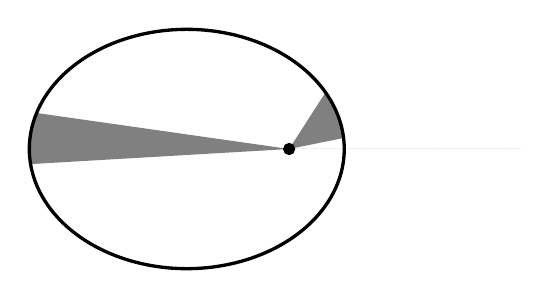
\begin{tikzpicture}[>=latex]
        \def\ecc{0.65}
        \def\SMA{2}
        \def\ap{\fpeval{\SMA*(1+\ecc)}}
        \def\pe{\fpeval{\SMA*(1-\ecc)}}
        \def\slr{\fpeval{\SMA*(1-\ecc^2)}}
        \def\thta{3}
        \def\thtb{0.2}
        \def\arca{0.2}
        \def\arcb{0.8}


        \fill[fill=gray] (0,0) -- ++(\thta:{3*cos(\thta r)}) plot[domain=\thta:\thta+\arca] (xy polar cs:angle=\x r,radius= {(\slr)/(1+\ecc*cos(\x r))})--(0,0)--cycle;
        \fill[fill=gray] (0,0) -- ++(\thtb:{3*cos(\thtb r)}) plot[domain=\thtb:\thtb+\arcb] (xy polar cs:angle=\x r,radius= {(\slr)/(1+\ecc*cos(\x r))})--(0,0)--cycle;

        \draw[domain=0:2*pi,samples=500, very thick] plot ({deg(\x)}:{(\slr)/(1+\ecc*cos(\x r))});

        \filldraw[] (0,0) circle (2pt);
    \end{tikzpicture}

    \caption{An orbit with multiple areas shaded, each of which is swept out in equal time}
\end{figure}

To prove this law, the area will be found of a segment of the ellipse tranversed from $t_1$ to $t_2$.
\begin{align*}
    \text{Area} & =\iint{}dA                                               \\
                & = \int_{\theta(t_1)}^{\theta(t_2)}\int_{0}^{r}rdrd\theta \\
                & = \int_{\theta(t_1)}^{\theta(t_2)}\frac{1}{2}r^2d\theta  \\
                & = \int_{t_1}^{t_2}\frac{1}{2}r^2\frac{d\theta}{dt}dt     \\
                & = \int_{t_1}^{t_2}\frac{1}{2}r^2\dot{\theta}dt           \\
\end{align*}

Recall from Equation \eqref{Angular Momentum:h unknown} that $h=r^2\dot{\theta}$.
\begin{align*}
    \text{Area} & = \int_{t_1}^{t_2}\frac{1}{2}r^2\dot{\theta}dt \\
                & = \int_{t_1}^{t_2}\frac{1}{2}hdt               \\
                & = \frac{h}{2}\int_{t_1}^{t_2}dt                \\
                & = \frac{h}{2}\Delta{}t                         \\
\end{align*}

This expression is expression is independent of where in the orbit a satellite is.
\begin{equation}\label{Kepler's First Law}
    \text{Area Traversed} = \frac{h}{2}\Delta{}t
\end{equation}

\bigskip\bigskip
\subsection{Conservation of Specific Energy}\label{sec:Conservation of Energy}

Specific energy $\varepsilon$ is, like angular momentum, conserved. It is defined as the sum of specific kinetic and specific potential energy.
\begin{align*}
    \varepsilon & =\frac{\text{KE}+\text{PE}}{m}                             \\
                & =\frac{1}{m}(\text{KE}+\text{PE})                          \\
                & =\frac{1}{m}\left(\frac{1}{2}mv^2+\frac{-\mu{}m}{r}\right) \\
\end{align*}
\begin{equation}\label{Specific Energy Physical}
    \varepsilon=\frac{v^2}{2}-\frac{\mu{}}{r}
\end{equation}

Conservation of energy can be proven quite simply with physical reasoning, as there is no external force (external to the system, with said system comprising of the orbited body and the orbiting body) to do work. With no external work done, there is no source of energy change. However, it can now be shown that specific energy is conserved through differentiation with respect to distance travelled. Recall that $a_r=\frac{-\mu}{r^2}$ (Equation \eqref{Differential Equation:r}) and $a_\theta=0$ (Equation \eqref{Differential Equation:theta}) from Section \ref{sec:Differential Equation Setup}.
\begin{align*}
    \frac{d\varepsilon}{ds} & =\frac{d}{ds}\left(\frac{|v|^2}{2}\right)-\frac{d}{ds}\left(\frac{\mu}{|r|}\right) \\
                            & =|v|\frac{d|v|}{ds}+\frac{\mu{}}{|r|^2}\frac{d|r|}{ds}                             \\
                            & =|v|\frac{d|v|}{dt}\frac{dt}{ds}+\frac{\mu{}}{|r|^2}\frac{d|r|}{dt}\frac{dt}{ds}   \\
                            & =\frac{dt}{ds}\left(|v|\frac{d|v|}{dt}+\frac{\mu{}}{|r|^2}\frac{d|r|}{dt}\right)   \\
                            & =\frac{dt}{ds}\left(|v|a_\parallel-a_r\frac{d|r|}{dt}\right)                       \\
                            & =\frac{dt}{ds}(|v|(\vv{a}\cdot\hat{v})-a_rv_r)                                     \\
                            & =\frac{dt}{ds}(\vv{a}\cdot\vv{v}-a_rv_r)                                           \\
                            & =\frac{dt}{ds}((a_rv_r+a_\theta{}v_\theta)-a_rv_r)                                 \\
                            & =\frac{dt}{ds}(a_\theta{}v_\theta)                                                 \\
                            & =\frac{dt}{ds}(0v_\theta)                                                          \\
                            & =0                                                                                 \\
\end{align*}

Because the derivative of $\varepsilon$ with respect to distance travelled is zero, it does not change across an orbit and will be conserved.

\pagebreak
\section{Orbit Geometry}\label{sec:Orbit geoemtry}

Various elements of an orbit can now be expressed simply. Note that there is a lot of variation in standards when it comes to hyperbolas and parabolas. In this document, the convention will be used that $a, c<0$ in a hyperbola. Note that $p$ is always positive. In a parabola, $a$ is infinite.

Throughout this section, it will be shown that an orbit can be defined uniquely by $a$ and $e$ (except for parabolic orbits).

\bigskip\bigskip
\subsection{Periapsis}\label{sec:Periapsis Geometric}

From Figure \ref{fig:Orbit Diagram}, a geometric observation can be made.
\begin{align*}
    r_\text{pe}+c+a & = 2a     \\
    r_\text{pe}     & =a-c     \\
                    & =a-ea    \\
                    & = a(1-e)
\end{align*}

TThis equation is valid for all elliptic and hyperbolic orbits, but not for parabolic ones (the semi-major axis of a parabola is infinite, while $1-e$ equals zero in a parabola).
\begin{equation}\label{Periapsis Radius Geometric}
    r_\text{pe}=a(1-e)
\end{equation}

\bigskip\bigskip
\subsection{Apoapsis}\label{sec:Apoapsis Geometric}

Using the same figure and similar observations and reasoning, the apoapsis radius can be found.
\begin{align*}
    r_\text{ap} & = a+c   \\
                & =a+ea   \\
                & =a(1+e)
\end{align*}

The apoapsis is not defined for hyperbolic or parabolic orbits.
\begin{equation}\label{Apoapsis Radius Geometric}
    r_\text{ap}=a(1+e)
\end{equation}

\bigskip\bigskip
\subsection{Semi-Minor Axis}\label{Sec:Semi Minor Axis Geometric}

The Semi-Minor Axis $b$ is slightly harder to find than the apoapsis and periapsis. Of course, various definitions of eccentricity can be applied, such as $e=\sqrt{1-\frac{a^2}{b^2}}$, to solve for $b$, however that's not quite intellectually fulfilling; after all, it's not immediately obvious where that equation came from.

Instead, the definition of an ellipse wil be brought in. In a circle, the distance to the center is always constant. In an ellipse, the sum of distances to the foci is always constant. This distance will be denoted $2d$.
\begin{align*}
    2d(\text{At Pe}) & = r_\text{pe}+(r_\text{ap}) \\
                     & = 2a                        \\
    d                & =a
\end{align*}

A right triangle can then be drawn with which further reasoning can be applied
\begin{figure}[H]
    \centering
    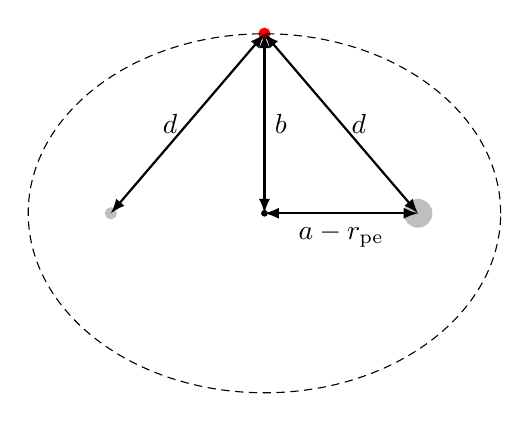
\begin{tikzpicture}[>=latex]
        \def\ecc{0.65}
        \def\SMA{3}
        \def\ap{\fpeval{\SMA*(1+\ecc)}}
        \def\pe{\fpeval{\SMA*(1-\ecc)}}
        \def\slr{\fpeval{\SMA*(1-(\ecc)^2)}}
        \def\SmA{\fpeval{\SMA*sqrt(1-\ecc^2)}}

        \filldraw[lightgray] (-\ap+\SMA,0) circle (2pt);
        \filldraw[lightgray] (-\SMA+\ap,0) circle (5pt);
        \filldraw[] (0,0) circle (1pt);
        \filldraw[red] (0,\SmA) circle (2pt);

        \draw[thin, densely dashed] (0,0) ellipse ({\SMA} and {\SmA});
        \draw[<->, thick] (0, 0) -- (\SMA-\pe, 0) node[midway, below] {$a-r_\text{pe}$};
        \draw[<->, thick] (0, 0) -- (0, \SmA) node[midway, right] {$b$};

        \draw[<->, thick] (-\ap+\SMA, 0) -- (0, \SmA) node[midway, left] {$d$};
        \draw[<->, thick] (\ap-\SMA, 0) -- (0, \SmA) node[midway, right] {$d$};

    \end{tikzpicture}

    \caption{An orbit with relevant parameters labeled, and with the point on the semi-major axis drawn in red}. The vacant focus is the smaller circle, with the orbited body being the large gray circle.
\end{figure}

The right triangle that will be examined is the one formed by the center of the orbit, the left focus, and the point in the orbit on the semi-minor axis. The Pythagorean Theorem can be applied to find the unknown $b$, keeping in mind that $d=a$.
\begin{align*}
    (a-r_\text{pe})^2+b^2 & = d^2                   \\
    (a-r_\text{pe})^2+b^2 & = a^2                   \\
    b^2                   & = a^2-(a-r_\text{pe})^2 \\
\end{align*}

Note from Figure \ref{fig:Orbit Diagram} that $r_\text{pe}+c=a$, meaning that $a-r_\text{pe}=c$, which in turn is defined as $c=ae$
\begin{align*}
    b^2 & = a^2-(c)^2         \\
    b^2 & = a^2-(ae)^2        \\
    b^2 & = a^2-a^2e^2        \\
    b^2 & = a^2(1-e^2)        \\
    b   & = \sqrt{a^2(1-e^2)} \\
    b   & = a\sqrt{1-e^2}     \\
\end{align*}

The semi-minor axis is not well defined for hyperbolic orbits. The argument of the square root can be put in an absolute value to ensure that the semi-minor axis is real. Note that for some hyperbolic orbits (namely where $e>\sqrt{2}$), $|b|>|a|$.

\begin{equation}\label{Semi Minor Axis Geometric}
    b=a\sqrt{|1-e^2|}
\end{equation}

\bigskip\bigskip
\subsection{Geometry in Terms of Measurable Parameters}\label{sec:Geometry in terms of Measurable Values}

While $e$ and $a$ are conventionally used as the defining parameters of an orbit, the apses can instead be used to describe elliptic orbits. Once $e$ and $a$ are known, other geometric parameters can be found as before. Hyperbolic and parabolic orbits do not have a defined apoapsis, so this does not apply to them.

\subsubsection{Semi-Major Axis in terms of Apses}
From Figure \ref{fig:Orbit Diagram}, $a$ can be found in terms of $r_\text{pe}$ and $r_\text{ap}$

\begin{align*}
    2a & = r_\text{pe}+r_\text{ap}
\end{align*}
\begin{equation}\label{SMA in terms of apses}
    a = \frac{r_\text{pe}+r_\text{ap}}{2}
\end{equation}

\subsubsection{Eccentricity in Terms of Apses}

The eccentricity can also be put in terms of $r_\text{ap}$ and $r_\text{pe}$ using Equations \eqref{Periapsis Radius Geometric} and \eqref{Apoapsis Radius Geometric}.
\begin{align*}
    r_\text{ap}             & =a(1+e) & r_\text{pe}             & =a(1-e) \\
    \frac{r_\text{ap}}{1+e} & =a      & \frac{r_\text{pe}}{1-e} & =a      \\
\end{align*}

Setting both sides equal to eachother,

\begin{align*}
    \frac{r_\text{ap}}{1+e}                                   & =\frac{r_\text{pe}}{1-e}                                                                         \\
    \frac{1+e}{r_\text{ap}}                                   & =\frac{1-e}{r_\text{pe}}                                                                         \\
    \frac{1}{r_\text{ap}}+\frac{e}{r_\text{ap}}               & =\frac{1}{r_\text{pe}}-\frac{e}{r_\text{pe}}                                                     \\
    \frac{e}{r_\text{ap}}+\frac{e}{r_\text{pe}}               & =\frac{1}{r_\text{pe}}-\frac{1}{r_\text{ap}}                                                     \\
    e\left(\frac{1}{r_\text{ap}}+\frac{1}{r_\text{pe}}\right) & =\frac{1}{r_\text{pe}}-\frac{1}{r_\text{ap}}                                                     \\
    e                                                         & =\frac{\frac{1}{r_\text{pe}}-\frac{1}{r_\text{ap}}}{\frac{1}{r_\text{pe}}+\frac{1}{r_\text{ap}}} \\
\end{align*}
\begin{equation}\label{Accentricity in terms of apses}
    e=\frac{r_\text{pe}^{-1}-r_\text{ap}^{-1}}{r_\text{pe}^{-1}+r_\text{ap}^{-1}}
\end{equation}

\bigskip\bigskip
\subsection{Conclusion}

Throughout this section, many geometric relationships have been found describing orbits. Most importantly, it has been shown that an orbital trajectory can be described in its plane using only two parameters: the semi-major axis $a$ and the eccentricity $e$. These relationships are summarized here.

\bigskip
The periapsis and apoapsis radii are
$$r_\text{pe}=a(1-e)\qquad\text{and}\qquad r_\text{ap}=a(1+e)$$

\bigskip
The semi-minor axis of the orbit is
$$b=a\sqrt{|1-e^2|}$$

\bigskip
The semi-major axis and eccentricity of an elliptic orbit can be stated in terms of known periapsis and apoapsis radii
$$a=\frac{r_\text{pe}+r_\text{ap}}{2}\qquad\qquad e=\frac{r_\text{pe}^{-1}-r_\text{ap}^{-1}}{r_\text{pe}^{-1}+r_\text{ap}^{-1}}$$

Because hyperbolas don't have physically meaningful apoapses, the semi-major axis and eccentricity can be defined in terms of the entry/exit angle $\theta_\text{hyp}$ and the periapsis radius.
$$e=\sec(\theta_\text{hyp})\qquad\qquad a=\frac{{r_\text{pe}}}{1-\sec(\theta_\text{hyp})}$$

\pagebreak
\section{Physical Orbital Parameters from Geometry}\label{Orbital Parameters from Geometry}
With the geometry of an entire orbit known, physical quantities can be determined.

\bigskip\bigskip
\subsection{Angular Momentum}\label{sec:Angular Momentum Geometric}

The angular momentum $h$ of a satellite is, as was proven earlier, conserved. From the physical definition of angular momentum ($\vv{h}=\vv{r}\times\vv{v}$), the following can be observed:
\begin{equation}\label{Angular Momentum Physical Definition}
    h=rv_\perp
\end{equation}

Equation \eqref{SLR h and mu}, which describes the semi-latus rectum from physical parameters, can be set equal to \eqref{SLR a and e}, which describes the semi-latus rectum from geometric definitions. This will allow for the angular momentum to be isolated.
\begin{align*}
    \frac{h^2}{\mu} & = a(1-e^2)           \\
    h^2             & = a(1-e^2)\mu        \\
    h               & = \sqrt{a\mu(1-e^2)} \\
\end{align*}

This equation is not defined for parabolic orbits. Note that in a hyperbolic orbit, the signs of $a$ and $1-e^2$ are both negative, so the square root is still real.
\begin{equation}\label{Angular Momentum Geometric Definition}
    h=\sqrt{a\mu(1-e^2)}
\end{equation}


\bigskip\bigskip
\subsection{Period}\label{Sec:Period Geometric}

The area of a closed ellipse is known from geometry.
$$\text{Area}=\pi{}ab$$

From Kepler's first law (which was proven in Section \ref{sec:Kepler's First Law}), an equation exists that tells us the area of an orbit as a function of time (Equation \eqref{Kepler's First Law}). If the entire period $T$ is used as the time step, then the area can be found. Because the period is not defined for a hyperbolic orbit, the semi-minor axis will not use an absolute value. However, it turns out that this omission is inconsequential anywho, as the $\sqrt{1-e^2}$ term will cancel out.
\begin{align*}
    \text{Area}          & = \frac{h}{2}P                                     \\
    \pi{}ab              & = \frac{h}{2}P                                     \\
    \pi{}a^2\sqrt{1-e^2} & = \frac{h}{2}P                                     \\
    \pi{}a^2\sqrt{1-e^2} & = \frac{\sqrt{a\mu(1-e^2)}}{2}P                    \\
    T                    & = \frac{2\pi{}a^2\sqrt{1-e^2}}{\sqrt{a\mu(1-e^2)}} \\
                         & = 2\pi{}a^2\sqrt{\frac{1-e^2}{a\mu(1-e^2)}}        \\
                         & = \sqrt{\frac{4\pi^2a^4}{a\mu}}                    \\
\end{align*}
\begin{equation}\label{Period Geometric}
    T = \sqrt{\frac{4\pi^2a^3}{\mu}}
\end{equation}

Hyperbolic and parabolic orbits do not have periods, as they are not closed.

\bigskip\bigskip
\subsection{Specific Energy}\label{sec:Specific Energy}

Specific energy $\varepsilon$ is the total energy in an orbit, normalized with respect to the mass of the satellite. Total energy is the sum of the kinetic energy and gravitational potential energy (with the potential constant set so that, as distance approaches infinity, the potential function vanishes).
\begin{align*}
    \varepsilon & =\frac{\text{KE}+\text{PE}}{m}                             \\
                & =\frac{1}{m}(\text{KE}+\text{PE})                          \\
                & =\frac{1}{m}\left(\frac{1}{2}mv^2+\frac{-\mu{}m}{r}\right) \\
                & =\frac{v^2}{2}-\frac{\mu{}}{r}                             \\
\end{align*}

Conservation of specific energy was proven earlier, but a more useful expression for it can be found.

Specific energy is constant, so it will be found at periapsis. First, velocity must be found by setting Equation \eqref{Angular Momentum Physical Definition} (the physical definition of angular momentum, $rv_\perp$) equal to its derived counterpart ($\sqrt{a\mu(1-e^2)}$) from Equation \eqref{Angular Momentum Geometric Definition}. Note that at periapsis, velocity is entirely normal to the radial vector, so $v_\perp=v$, and recall that Equation \eqref{Periapsis Radius Geometric} states $r_\text{pe}=a(1-e)$.
\begin{align*}
    r_\text{pe}v_\text{pe} & = \sqrt{\mu{}a(1-e^2)}                       \\
    a(1-e)v_\text{pe}      & = \sqrt{\mu{}a(1-e)(1+e)}                    \\
    v_\text{pe}            & = \sqrt{\frac{\mu{}a(1-e)(1+e)}{a^2(1-e)^2}} \\
    v_\text{pe}            & = \sqrt{\frac{\mu{}(1+e)}{a(1-e)}}           \\
\end{align*}

Now, specific energy can be found.
\begin{align*}
    \varepsilon & = \frac{1}{2}v^2-\frac{\mu}{r}                            \\
                & = \frac{1}{2}\frac{\mu{}(1+e)}{a(1-e)}-\frac{\mu}{a(1-e)} \\
                & = \frac{\mu{}(1+e)}{2a(1-e)}-\frac{2\mu}{2a(1-e)}         \\
                & = \frac{\mu{}(1+e)-2\mu}{2a(1-e)}                         \\
                & = \frac{\mu{}(e-1)}{2a(1-e)}                              \\
                & = \frac{-\mu}{2a}                                         \\
\end{align*}

Note that because $a$ is infinite for a parabola (see \ref{sec:Analysis of parabolic trajectories}), $\varepsilon=0$ for parabolic orbits, Since $a<0$ for hyperbolas, $\varepsilon>0$ in hyperbolic orbits.
\begin{equation}\label{Specific Energy Geometric}
    \varepsilon=\frac{-\mu}{2a}
\end{equation}

This is valid for \textit{all} orbits. Of note is the fact that eccentricity plays no role in specific energy of an orbit, aside from to determine its sign in extreme cases. This has an interesting ramification for orbital dynamics; since a burn normal to the velocity vector and in plane with the orbit performs no work, it must not change the specific energy of the orbit. While other parameters, such as inclination, can change without the specific energy changing, that requires out-of-plane maneuvers. This implies (correctly) that burning normal to the velocity has the effect of changing its eccentricity or inclination but not its semi-major axis.

\bigskip\bigskip
\subsection{Velocity}\label{sec:Velocity}

Specific energy found in Equation \eqref{Specific Energy Geometric} can be set equal to the physical definition of specific energy, so that $v$ can be solved for.
\begin{align*}
    \frac{1}{2}v^2-\frac{\mu}{r} & =\frac{-\mu}{2a}                     \\
    \frac{1}{2}v^2               & =\frac{\mu}{r}-\frac{\mu}{2a}        \\
    v^2                          & =\frac{2\mu}{r}-\frac{\mu}{a}        \\
    v                            & =\sqrt{\frac{2\mu}{r}-\frac{\mu}{a}} \\
\end{align*}

The $\frac{-\mu}{a}$ term vanishes in parabolic orbits, showing that in a parabolic orbit velocity is determined solely by radius (and is independent of periapsis). In a hyperbolic orbit, both terms in the square root are positive, showing that velocity at a given radius is greater in a hyperbolic orbit than in a parabolic or elliptic orbit.
\begin{equation}\label{Vis-Viva Equation}
    v= \sqrt{\frac{2\mu}{r}-\frac{\mu}{a}}
\end{equation}

This equation describes velocity of a satellite as a function of its distance from the orbited body, the semi-major axis of its orbit, and the standard gravitational parameter. Note that it is defined for elliptic, parabolic, and hyperbolic orbits.

For circular orbits where $a=r$, this simplifies to
\begin{equation}\label{Circular Velocity}
    v_\text{circ} = \sqrt{\frac{\mu}{r}}
\end{equation}

Escape is achieved when a satellite is able to approach infinite distance with a real-valued velocity. The minimum such velocity that the satellite can approach is zero. From Equation \eqref{Vis-Viva Equation}, this can only happen if $a$ is infinite. This gives escape velocity as a function of radius to be
\begin{equation}\label{Escape velocity}
    v_\text{esc}=\sqrt{\frac{2\mu}{r}}
\end{equation}

\bigskip\bigskip
\subsection{Flight Path Angle}

The flight path angle $\phi$ is the angle between a satellite's velocity vector and the line (in plane with the orbit) tangent to the orbited body (in other words, the angle between $\vv{v}$ and $\hat{u}_\theta$).

\begin{figure}[H]
    \centering
    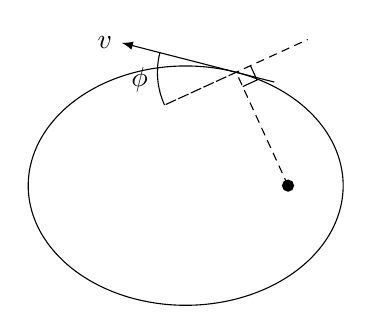
\begin{tikzpicture}[>=latex]
        \def\ecc{0.65}
        \def\SMA{2}
        \def\thta{2}
        \def\ap{\fpeval{\SMA*(1+\ecc)}}
        \def\pe{\fpeval{\SMA*(1-\ecc)}}
        \def\slr{\fpeval{\SMA*(1-\ecc^2)}}
        \def\arcRad{1}
        \def\Ra{\fpeval{\slr/(1+\ecc*cos(\thta))}}
        \def\yAB{\fpeval{sin(\thta)*\Ra}}
        \def\xB{\fpeval{(2*\SMA*\ecc)+cos(\thta)*\Ra}}
        \def\thtaA{\fpeval{pi-\thta}}
        \def\thToPt{\fpeval{(-\thtaA+atan(\yAB/\xB))/2}}

        \coordinate (pt) at ({deg(\thta)}:{\slr/(1+\ecc*cos(\thta r))}) {};
        \coordinate (o) at (\SMA-\pe,0) {};

        \draw[densely dashed] (0,0) -- (pt);

        \draw[domain=0:2*pi,samples=500, thin] plot ({deg(\x)}:{(\slr)/(1+\ecc*cos(\x r))});
        \draw[densely dashed] (pt) -- +({deg(\thta)+90}:1)-- +({deg(\thta)-90}:1);
        \draw[thin] (pt)++({deg(\thta)+180}:0.2)-- ++({deg(\thta)-90}:0.2)-- ++({deg(\thta)}:0.2);
        \draw[->] (pt) -- +({deg(\thToPt)}:0.5)--+({deg(\thToPt)-180}:1.5) node[left] {$\vv{v}$};

        \draw[] (pt)+({deg(\thta)+90}:\arcRad) arc ({deg(\thta)+90}:{deg(\thToPt)+180}:\arcRad) node[midway, left] {$\phi$};

        \filldraw[] (0,0) circle (2pt);
    \end{tikzpicture}
    \caption{An orbit with the flight path angle $\phi$ indicated}
\end{figure}

Angular momentum (Equations \eqref{Angular Momentum Geometric Definition} and \eqref{Angular Momentum Physical Definition}) can be used to find $\phi$.
\begin{align*}
    rv_\perp                                       & = \sqrt{a\mu(1-e^2)}                                       \\
    rv\cos(\phi)                                   & = \sqrt{a\mu(1-e^2)}                                       \\
    r\cos(\phi)\sqrt{\frac{2\mu}{r}-\frac{\mu}{a}} & = \sqrt{a\mu(1-e^2)}                                       \\
    \cos(\phi)\sqrt{2r\mu-\frac{r^2\mu}{a}}        & = \sqrt{a\mu(1-e^2)}                                       \\
    \cos(\phi)                                     & = \frac{\sqrt{a\mu(1-e^2)}}{\sqrt{2r\mu-\frac{r^2\mu}{a}}} \\
    \cos(\phi)                                     & = \sqrt{\frac{a\mu(1-e^2)}{2r\mu-\frac{r^2\mu}{a}}}        \\
    \cos(\phi)                                     & = \sqrt{\frac{a^2(1-e^2)}{2ra-r^2}}                        \\
    \cos(\phi)                                     & = \sqrt{\frac{a^2(1-e^2)}{r(2a-r)}}
\end{align*}

Note that even in hyperbolic orbits the argument of the square root is positive, so $\cos(\phi)$ is always real. $\phi$ can be found with an arccosine, keeping in mind that arccosine loses a solution. $\phi$ is positive when the satellite is getting further from the orbited body, and negative when it's getting closer. Therefore, the sign of $\phi$ is the same as the sign as $\vv{r}\cdot\vv{v}$
\begin{equation}\label{Flight Path Angle}
    \phi=\arccos{\sqrt{\frac{a^2(1-e^2)}{r(2a-r)}}}
\end{equation}


An equation has already been found relating $r$ and $\theta$, meaning this formula \textit{can} be put in terms of $\theta$. Solving for this expression, however, is left as an exercise to the reader.

\bigskip\bigskip
\subsection{True Anomaly}
Using the orbit equation (Equation \eqref{Polar Final}), the angle $\theta$ to the periapsis can be found.
\begin{align*}
    r               & =\frac{a(1-e^2)}{1+e\cos(\theta)} \\
    1+e\cos(\theta) & =\frac{a(1-e^2)}{r}               \\
    \cos(\theta)    & =\frac{a(1-e^2)}{er}-\frac{1}{e}  \\
\end{align*}

When taking the inverse cosine, a solution will be lost. On the side of the orbit where $r$ is increasing (moving from periapsis to apoapsis) we know that $0<\theta<\pi$, while on the other side of the orbit $\pi<\theta<2\pi$. Therefore, the sign of $\theta$ (assuming $-\pi<\theta<\pi$ is taken to the the domain) is the same as the sign of $v_r$, which in turn is the same as the sign of $\vec{v}\cdot\vec{r}$.

\begin{equation}\label{True Anomoly Geometric}
    \theta=\cos^{-1}\left(\frac{a(1-e^2)-r}{er}\right)
\end{equation}

\bigskip\bigskip
\subsection{Conclusion}

Throughout this section, many geometric relationships have been found describing orbits. Most importantly, it has been shown that an orbital trajectory can be described in its plane using only two parameters: the semi-major axis $a$ and the eccentricity $e$. These relationships are summarized here.

\bigskip
The angular momentum is
$$h=\sqrt{a\mu(1-e^2)}$$

\bigskip
The specific energy of an orbit is
$$\varepsilon=\frac{v^2}{2}-\frac{\mu}{r}=\frac{-\mu}{2a}$$

\bigskip
The period of an elliptic orbit is
$$P=\sqrt{\frac{4\pi^2a^3}{\mu}}$$

\bigskip
The velocity at any point in an orbit can be found with
$$v=\sqrt{\frac{2\mu}{r}-\frac{\mu}{a}}$$

Velocity for circular orbit is
$$v_\text{circ}=\sqrt{\frac{\mu}{r}}$$

Escape velocity at any altitude is
$$v_\text{esc}=\sqrt{\frac{2\mu}{r}}=v_\text{circ}\sqrt{2}$$

\bigskip
While the flight path angle can be found as
$$\phi=\arccos\left(\sqrt{\frac{a^2(1-e^2)}{r(2a-r)}}\right)$$

\bigskip
The true anomaly can be found in an orbit with
$$\theta=\arccos\left(\frac{a(1-e^2)-r}{er}\right)$$

\pagebreak
\section{Geometry from Physical Parameters}

A plausible scenario for a spacecraft is that telemetry systems provide a distance from the orbited planet and current velocity (as a vector in $\vec{u}_r$ and $\vec{u}_\theta$, noting that $v_n=0$ at all points), while measured or estimated values of $\mu$ would be known. In this case, equations so far derived in terms of geometric values such as $a$ and $e$ will prove widely useless until the precise orbit of the spacecraft is known. Therefore, equations will be derived in terms of these physical values to determine geometric parameters of the orbit. Throughout this chapter, $v$ will be used to refer to the magnitude of $\vv{v}$, while $v_r$ and $v_\theta$, and $\phi$ may also be used. Note that $\phi$ can be found using the fact that $v_\theta=v\cos(\phi)$ so $\phi=\arccos(v_\theta/v)$, with the sign of $\phi$ being the same as the sign of $v_r$.

\bigskip\bigskip
\subsection{Orbit Shape}

Many parameters will depend on the type of orbit that a satellite is in. As such, an easy way of determining this must be found. Section \ref{sec:Specific Energy}, specifically Equation \eqref{Specific Energy Physical} defined specific energy to be
$$\varepsilon=\frac{1}{2}v^2-\frac{\mu}{r}$$

For an orbit to be hyperbolic, the satellite must be able to approach infinite distance from the orbited body, with the velocity always remaining positive. This means the kinetic energy term must be greater in magnitude than the potential energy term, thus making the specific energy positive. For the orbit to be parabolic, the satellite's velocity will approach zero as its distance approaches infinity. This requires the kinetic and potential energy terms to have the same magnitude, making specific energy zero. For a closed orbit, the satellite cannot approach infinite distance without kinetic energy being negative. This means the kinetic term is less than the potential term, making elliptic orbit specific energy negative. This can be summarized with the following statement
\begin{equation}\label{Orbit Shape Physical}
    \text{Orbit Shape}: \begin{cases}
        \text{Elliptic}   & v<\sqrt{\frac{2\mu}{r}} \\
        \text{Parabolic}  & v=\sqrt{\frac{2\mu}{r}} \\
        \text{Hyperbolic} & v>\sqrt{\frac{2\mu}{r}}
    \end{cases}
\end{equation}

Note that it is astronomically (I will not apologize for that) improbable for an orbit to be parabolic, given that there is only one exact state for a parabolic orbit and any deviation from that state will result in an elliptic or hyperbolic orbit.

This can be used to prove an interesting relationship
\begin{align*}
    \varepsilon & = \frac{1}{2}v^2-\frac{\mu}{r}                                     \\
                & = \frac{1}{2}\left(v^2-\frac{\mu}{2r}\right)                       \\
                & = \frac{1}{2}\left(v^2-\left(\sqrt{\frac{\mu}{2r}}\right)^2\right) \\
                & = \frac{1}{2}\left(v^2-v_\text{escape}^2\right)                    \\
\end{align*}

While this may not be immediately useful, it is nonetheless intriguing.

\bigskip\bigskip
\subsection{Semi-Major Axis}\label{sec:SMA in Terms of V,R}

If $v$ and $r$ are known, Equation \eqref{Vis-Viva Equation} can be solved for $a$.

\begin{align*}
    v                  & = \sqrt{\frac{2\mu}{r}-\frac{\mu}{a}} \\
    v^2                & = \frac{2\mu}{r}-\frac{\mu}{a}        \\
    v^2-\frac{2\mu}{r} & =-\frac{\mu}{a}                       \\
    \frac{\mu}{a}      & = \frac{2\mu}{r}-v^2                  \\
    \frac{a}{\mu}      & = \frac{1}{\frac{2\mu}{r}-v^2}        \\
    a                  & = \frac{\mu}{\frac{2\mu}{r}-v^2}      \\
    a                  & = \frac{\mu r}{2\mu-rv^2}             \\
\end{align*}

Note that $\frac{2\mu}{r}-v^2=v_\text{esc}^2-v^2$.

\begin{equation}\label{SMA in terms of r, v}
    a=\frac{\mu r}{2\mu-rv^2}=\frac{\mu}{v_\text{esc}^2-v^2}
\end{equation}

This shows that the semi-major axis of an orbit is inversely proportional to the difference between the squares of escape velocity and current velocity. This also implies that this difference is conserved throughout an orbit.

\bigskip\bigskip
\subsection{Eccentricity}\label{sec:Eccentricity in Terms of V,R}

To determine the eccentricity at any point given $v$, $r$, and $\phi$, angular momentum must be used.

\begin{align*}
    \sqrt{a\mu(1-e^2)}                & =h                                            \\
    \sqrt{a\mu(1-e^2)}                & =rv\cos(\phi)                                 \\
    a\mu(1-e^2)                       & =r^2v^2\cos^2(\phi)                           \\
    \frac{\mu r}{2\mu-rv^2}\mu(1-e^2) & =r^2v^2\cos^2(\phi)                           \\
    \mu(1-e^2)                        & =r^2v^2\cos^2(\phi)\frac{2\mu-rv^2}{\mu r}    \\
    1-e^2                             & =r^2v^2\cos^2(\phi)\frac{2\mu-rv^2}{\mu^2r}   \\
    e^2                               & =1-r^2v^2\cos^2(\phi)\frac{2\mu-rv^2}{\mu^2r} \\
\end{align*}

\begin{equation}
    e=\sqrt{1-r^2v^2\cos^2(\phi)\frac{2\mu-rv^2}{\mu^2r}}
\end{equation}

\bigskip\bigskip
\subsection{Conclusion}

\bigskip
An orbit can take one of three shapes. If the velocity is $v<\sqrt{\frac{2\mu}{r}}$, the orbit is elliptic. If $v=\sqrt{\frac{2\mu}{r}}$ the orbit is parabolic. If the velocity is above escape velocity $v>\sqrt{\frac{2\mu}{r}}$, then the trajectory is be hyperbolic.

\bigskip
The semi-major axis $a$ can be found from measured values
$$a=\frac{\mu r}{2\mu-rv^2}=\frac{\mu}{v_\text{esc}^2-v^2}$$

\bigskip
The eccentricity is
$$e=\sqrt{1-r^2v^2\cos^2(\phi)\frac{2\mu-rv^2}{\mu^2r}}$$

With the two defining geometric parameters able to be determined from instrumentation readings, equations from Sections \ref{sec:Orbit geoemtry} and \ref{Orbital Parameters from Geometry} can be used.

\begin{comment}
\bigskip\bigskip
\subsection{Apsis Radii}
The radii of the apses (periapsis and apoapsis) can be found using a combination of conservation of energy and conservation of angular momentum. The angular momentum at any point is $h=rv_\theta$. Using this, an expression can be found for the radii of the apses (keeping in mind that at periapsis and apoapsis, the velocity is entirely along the horizontal with $\phi=0$).

Beginning with conservation of momentum,
\begin{align*}
    h_\text{aps}             & = h        \\
    r_\text{aps}v_\text{aps} & =rv_\theta \\
\end{align*}
\begin{equation}\label{Apses Radius from h}
    v_\text{aps}=\frac{rv_\theta}{r_\text{aps}}
\end{equation}

Switching now to conservation of energy,
\begin{align*}
    \frac{1}{2}v_\text{aps}^2-\frac{\mu}{r_\text{aps}} & =\frac{1}{2}v^2-\frac{\mu}{r}                 \\
    v_\text{aps}^2                                     & =v^2-\frac{2\mu}{r}+\frac{2\mu}{r_\text{aps}} \\
\end{align*}
\begin{equation}\label{Apses Velocity from Radius}
    v_\text{aps}=\sqrt{v^2-\frac{2\mu}{r}+\frac{2\mu}{r_\text{aps}}}
\end{equation}

Setting \eqref{Apses Velocity from Radius} and \eqref{Apses Radius from h} equal to each other,
\begin{align*}
    \frac{rv_\theta}{r_\text{aps}}       & = \sqrt{v^2-\frac{2\mu}{r}+\frac{2\mu}{r_\text{aps}}}                            \\
    \frac{r^2v_\theta^2}{r_\text{aps}^2} & = v^2-\frac{2\mu}{r}+\frac{2\mu}{r_\text{aps}}                                   \\
    r^2v_\theta^2                        & = v^2r_\text{aps}^2-\frac{2\mu}{r}r_\text{aps}^2+2\mu{}r_\text{aps}              \\
    0                                    & = \left(\frac{2\mu}{r}-v^2\right)r_\text{aps}^2-2\mu{}r_\text{aps}+r^2v_\theta^2 \\
\end{align*}

This equation is quadratic in $r_\text{aps}$ and can be solved
\begin{align*}
    r_\text{aps} & =\frac{2\mu\pm\sqrt{(2\mu)^2-4(\frac{2\mu}{r}-v^2)(r^2v_\theta^2)}}{2(\frac{2\mu}{r}-v^2)} \\
                 & =\frac{2\mu\pm\sqrt{4\mu^2-4(2\mu{}rv_\theta^2-v^2r^2v_\theta^2)}}{2(\frac{2\mu}{r}-v^2)}  \\
                 & =\frac{2\mu\pm2\sqrt{\mu^2-2\mu{}rv_\theta^2+v^2r^2v_\theta^2}}{2(\frac{2\mu}{r}-v^2)}     \\
                 & =\frac{\mu\pm\sqrt{\mu^2-2\mu{}rv_\theta^2+(rvv_\theta)^2}}{\frac{2\mu}{r}-v^2}            \\
                 & =\frac{\mu{}r\pm{}r\sqrt{\mu^2-2\mu{}rv_\theta^2+(rvv_\theta)^2}}{2\mu-rv^2}               \\
\end{align*}

The substitution will now be made that $v_\theta=v\cos(\phi)$
\begin{align*}
    r_\text{aps} & =\frac{\mu{}r\pm{}r\sqrt{\mu^2-2\mu{}rv^2\cos^2(\phi)+(rvv\cos(\phi))^2}}{2\mu-rv^2}  \\
                 & =\frac{\mu{}r\pm{}r\sqrt{\mu^2-2\mu{}rv^2\cos^2(\phi)+r^2v^4\cos^2(\phi)}}{2\mu-rv^2} \\
\end{align*}
\begin{equation}\label{Aspes Quadratic Solution}
    r_\text{aps}=\frac{\mu{}r\pm{}r\sqrt{\mu^2-rv^2(2\mu-rv^2)\cos^2{\phi}}}{2\mu-rv^2}
\end{equation}

A parameter $Q$ will be defined as the square of the ratio between true velocity at any altitude and velocity required for circular orbit at that altitude.
$$Q=(\frac{v}{\sqrt{\mu/r}})^2=\frac{v^2r}{\mu}$$

Solved for $v$, $v=\sqrt{Q\frac{\mu}{r}}$

\begin{align*}
    r_\text{aps} & =\frac{\mu{}r\pm{}r\sqrt{\mu^2-rv^2\cos^2{\phi}(2\mu-rv^2)}}{2\mu-rv^2}                                                                   \\
                 & =\frac{\mu{}r\pm{}r\sqrt{\mu^2-r(\sqrt{Q\frac{\mu}{r}})^2\cos^2{\phi}(2\mu-r(\sqrt{Q\frac{\mu}{r}})^2)}}{2\mu-r(\sqrt{Q\frac{\mu}{r}})^2} \\
                 & =\frac{\mu{}r\pm{}r\sqrt{\mu^2-Q\mu^2\cos^2{\phi}(2-Q)}}{2\mu-Q\mu}                                                                       \\
                 & =\frac{r\pm{}r\sqrt{1-Q(2-Q)\cos^2{\phi}}}{2-Q}                                                                                           \\
\end{align*}
\begin{equation}\label{Apses Quadratic Solution with Q}
    r_\text{aps}=\frac{r\pm{}r\sqrt{1-Q(2-Q)\cos^2{\phi}}}{2-Q}
\end{equation}

Equation \eqref{Apses Quadratic Solution with Q} is not in and of itself all that useful, however it allows more exploration of the limitations of Equation \eqref{Aspes Quadratic Solution}.

Equation \eqref{Orbit Shape Physical} can be used to determine how $Q$ depends on the shape of the orbit. For an elliptic orbit $0<Q<2$. For a parabolic orbit $Q=2$. For a hyperbolic orbit, $Q>2$.

In an elliptic orbit where $0<Q<2$, it can be found that $0<Q(2-Q)\cos^2\phi<1$, so $r\sqrt{1-Q(2-Q)\cos^2\phi}$ is strictly positive with magnitude less $r$. Because the denominator is strictly positive, the apoapsis radius is given by the $+$ side of $\pm$ while the periapsis radius is given by the $-$ side.

In a parabolic orbit $Q=2$, making the denominator zero. This means that another method of determining periapsis must be analyzed.

In a hyperbolic orbit in which $Q>2$, $Q(2-Q)\cos^2\phi<0$, so $r\sqrt{1-Q(2-Q)\cos^2\phi}$ is strictly positive with magnitude greater than $r$. Unlike in an elliptic orbit, the denominator will be negative, meaning the numerator should also be negative for a positive (and therefore meaningful) periapsis. This means that, once again, the periapsis is given by the $-$ side of $\pm$.

Equation \eqref{Aspes Quadratic Solution} will be rewritten more concisely as
\begin{equation}\label{Periapsis and Apoapsis Radii}
    [r_\text{pe}, r_\text{ap}]=\frac{\mu{}r\mp{}r\sqrt{\mu^2-rv_\theta^2(2\mu{}+rv^2)}}{2\mu-rv^2}
\end{equation}

Note that this equation's results are only as valid is the data inputted+; if bogus data is thrown in, then the result will be equally meaningless. If $v_\theta$ is measured as greater than $v$, then the solution to this equation will have the entire orbit occuring either above or below the measured altitude. Similarly, the apoapsis height for a hyperbola cannot be used for any meaningful analysis, and should be neglected. Finally, this equation will fail to yield any result at all for perfectly parabolic orbits.

\subsubsection{Parabola Periapsis}

The perapsis of a parabolic orbit must be found with different means than that of a hyperbolic or elliptic orbit. Recall from Equation \eqref{Orbit Shape Physical} that in a parabolic orbit, $v=\sqrt\frac{2\mu}{r}$. For angular momentum to be conserved
\begin{align*}
    r_\text{pe}v_\text{pe} & =rv_\theta                                         \\
    r_\text{pe}            & =\frac{rv_\theta}{v_\text{pe}}                     \\
                           & =\frac{rv_\theta}{\sqrt{\frac{2\mu}{r_\text{pe}}}} \\
    r_\text{pe}^2          & =\frac{r^2v_\theta^2}{\frac{2\mu}{r_\text{pe}}}    \\
    r_\text{pe}^2          & =\frac{r_\text{pe}r^2v_\theta^2}{2\mu}             \\
\end{align*}
\begin{equation}\label{Periapsis Radius Parabola}
    r_\text{pe,parabola}=\frac{r^2v_\theta^2}{2\mu}
\end{equation}

\bigskip\bigskip
\subsection{Velocity as a Function of Radius}

The velocity at any point an in orbit can be found using conservation of energy and momentum. A subscript 0 will be used to signify an initial measurement, to allow clear distinction between $v$, the velocity at any arbitrary point, and $v_0$, the current measured velocity of the satellite.

Conservation of energy will be applied first
\begin{align*}
    \varepsilon                  & =\varepsilon_0                                           \\
    \frac{1}{2}v^2-\frac{\mu}{r} & =\frac{1}{2}v_0^2-\frac{\mu}{r_0}                        \\
    v^2                          & =v_0^2-\frac{2\mu}{r_0}+\frac{2\mu}{r}                   \\
    v                            & =\sqrt{v_0^2-2\mu\left(\frac{1}{r_0}+\frac{1}{r}\right)} \\
\end{align*}

Using conservation of momentum, this can be further expressed as a vector
\begin{align*}
    h         & =h_0                        \\
    rv_\theta & =r_0v_{\theta{}0}           \\
    v_\theta  & =\frac{r_0v_{\theta{}0}}{r} \\
\end{align*}

Knowing that $v^2=v_r^2+v_\theta^2$, the missing component $v_r$ can be found.
\begin{align*}
    v^2                                              & =v_r^2+v_\theta^2                                                                                  \\
    v_0^2-2\mu\left(\frac{1}{r_0}+\frac{1}{r}\right) & =v_r^2+\left(\frac{r_0v_{\theta{}0}}{r}\right)^2                                                   \\
    v_r^2                                            & =v_0^2-2\mu\left(\frac{1}{r_0}+\frac{1}{r}\right)-\left(\frac{r_0v_{\theta{}0}}{r}\right)^2        \\
    v_r                                              & =\sqrt{v_0^2-2\mu\left(\frac{1}{r_0}+\frac{1}{r}\right)-\left(\frac{r_0v_{\theta{}0}}{r}\right)^2} \\
\end{align*}

The velocity vector is therefore
\begin{equation}\label{Velocity Vector}
    \begin{aligned}
        \vv{v} & =\frac{r_0v_{\theta{}0}}{r}\hat{u}_\theta                                                                   \\
               & +\sqrt{v_0^2-2\mu\left(\frac{1}{r_0}+\frac{1}{r}\right)-\left(\frac{r_0v_{\theta{}0}}{r}\right)^2}\hat{u}_r \\
               & +0\hat{u}_n
    \end{aligned}
\end{equation}

Or, written as a magnitude,
\begin{equation}\label{Velocity Magnitude}
    v=\sqrt{v_0^2-2\mu\left(\frac{1}{r_0}+\frac{1}{r}\right)}
\end{equation}


\bigskip\bigskip
\subsection{Flight Path Angle at Any Point}

The simplest expression would be for $\phi$ as a function of $v$, however for the sake of consistency with equations \eqref{Velocity Vector} and \eqref{Velocity Magnitude}, the flight path angle will instead be found as a function of radius. Both $v$ and $v_\theta$, are known, so from trigonometry $\phi$ can be found.

\begin{figure}[H]
    \centering
    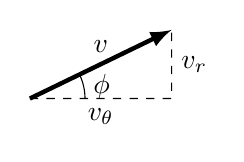
\begin{tikzpicture}[>=latex]
        \def\vel{2}
        \def\velThta{1.8}
        \def\phiAng{\fpeval{acos(\velThta/\vel)}}
        \def\arcRad{0.7}

        \draw[->, ultra thick] (0,0) -- ({deg(\phiAng)}:\vel) node[midway,above] {$v$};
        \draw[dashed] (0,0) -- (\velThta,0) node[midway,below] {$v_\theta$} -- ({deg(\phiAng)}:\vel) node[midway, right] {$v_r$};
        \draw[] (\arcRad,0) arc (0:{deg(\phiAng)}:\arcRad) node[midway, right] {$\phi$};
    \end{tikzpicture}
    \caption{Diagram showing the components of $v$}\label{fig:Velocity Triangle}
\end{figure}

From Figure \ref{fig:Velocity Triangle}, three trigonometric identities can be found.
\begin{align*}
    \cos{\phi}=\frac{v_\theta}{v} \\
    \sin{\phi}=\frac{v_r}{v}      \\
    \tan{\phi}=\frac{v_r}{v_\theta}
\end{align*}

Because the $v$ and $v_\theta$ terms are shortest, the cosine will be used.
\begin{align*}
    \cos(\phi) & = \frac{v_\theta}{v}                                                                 \\
               & = \frac{r_0v_{\theta{}0}/r}{\sqrt{v_0^2-2\mu\left(\frac{1}{r_0}+\frac{1}{r}\right)}} \\
               & = \frac{r_0v_{\theta{}0}}{r\sqrt{v_0^2-2\mu\left(\frac{1}{r_0}+\frac{1}{r}\right)}}  \\
\end{align*}
\begin{equation}\label{Flight Path Angle Physical}
    \phi=\cos^{-1}\left(\frac{r_0v_{\theta{}0}}{r\sqrt{v_0^2-2\mu(\frac{1}{r_0}+\frac{1}{r})}}\right)
\end{equation}

\bigskip\bigskip
\subsection{Geometric Parameters}

Until this point, this section has worked purely with physical quantities instead of the geometric ones already defined. However, it is at this point that geometric identities must be defined in terms of physically measured bases.

\subsubsection{Semi-Major Axis}\label{sec:SMA Physical}

From Figure \ref{fig:Orbit Diagram}, the major axis is the sum of the apoapsis and periapsis radii. Therefore,
\begin{align*}
    2a & = r_\text{pe}+r_\text{ap}                                          \\
       & =\frac{\mu{}r-{}r\sqrt{\mu^2-rv_\theta^2(2\mu{}+rv^2)}}{2\mu-rv^2} \\
       & +\frac{\mu{}r+{}r\sqrt{\mu^2-rv_\theta^2(2\mu{}+rv^2)}}{2\mu-rv^2} \\
       & =\frac{2\mu{}r}{2\mu-rv^2}                                         \\
\end{align*}

Dividing both sides by two, this leaves
\begin{align}\label{SMA Physical}
    a = \frac{\mu{}r}{2\mu-rv^2}
\end{align}

An equivalent form of this equation can be found.

\begin{align*}
    a & = \frac{\mu{}r}{2\mu-rv^2}         \\
    a & = \frac{\mu{}}{\frac{2\mu}{r}-v^2}
\end{align*}

Recall from Equation \eqref{Orbit Shape Physical} that escape velocity is $v_\text{esc}=\sqrt{2\mu/r}$
\begin{align}\label{SMA Physical Escape Velocity}
    a = \frac{\mu{}}{v_\text{esc}^2-v^2}
\end{align}

This shows that the semi-major axis of an orbit is inversely proportional to the difference between the square of the escape velocity and the current velocity.

\subsubsection{Eccentricity}\label{sec:Eccentricity physical}

Recall from Equation \eqref{Angular Momentum Geometric Definition} that
$$h=\sqrt{a\mu{}(1-e^2)}$$

Equation \eqref{Angular Momentum Physical Definition} adds that
$$h=rv_\perp=rv_\theta$$

These can be set equal to eachother and solved for $e$.
\begin{align*}
    \sqrt{a\mu{}(1-e^2)}                 & = rv_\theta                                       \\
    a\mu{}(1-e^2)                        & = r^2v_\theta^2                                   \\
    \frac{\mu{}r}{2\mu-rv^2}\mu{}(1-e^2) & = r^2v_\theta^2                                   \\
    \frac{\mu^2r}{2\mu-rv^2}(1-e^2)      & = r^2v_\theta^2                                   \\
    1-e^2                                & = \frac{r^2v_\theta^2(2\mu-rv^2)}{\mu^2r}         \\
    e^2                                  & =1-\frac{r^2v_\theta^2(2\mu-rv^2)}{\mu^2r}        \\
    e                                    & =\sqrt{1-\frac{r^2v_\theta^2(2\mu-rv^2)}{\mu^2r}} \\
    e                                    & =\sqrt{1-\frac{rv_\theta^2(2\mu-rv^2)}{\mu^2}}
\end{align*}
\begin{equation}\label{Eccentricity Physical}
    e=\sqrt{1-\frac{rv_\theta^2(2\mu-rv^2)}{\mu^2}} \\
\end{equation}

With both Semi-Major Axis and Eccentricity calculated in terms of physical inputs, any geometric relationships can be expressed in terms of physical inputs. Equations \eqref{SMA Physical} and \eqref{Eccentricity Physical} allow equations such as the orbit equation to be put int terms of physically measured values.

\bigskip\bigskip
\subsection{Period}
Unfortunately, the most efficient way of finding the period from physical inputs is to rewrite Equation \eqref{Period Geometric} from \ref{Sec:Period Geometric} in terms of the semi-major axis found in Section \ref{sec:SMA Physical} (Equation \eqref{SMA Physical}).
\begin{align*}
    P & = \sqrt{\frac{4\pi^2a^3}{\mu}}                          \\
      & = \sqrt{\frac{4\pi^2(\frac{\mu{}r}{2\mu-rv^2})^3}{\mu}} \\
      & = \sqrt{\frac{4\pi^2\mu^3r^3}{\mu(2\mu-rv^2)^3}}        \\
      & = \sqrt{\frac{4\pi^2\mu^2r^3}{(2\mu-rv^2)^3}}           \\
      & = 2\pi\mu\sqrt{\frac{r^3}{(2\mu-rv^2)^3}}               \\
      & = 2\pi\mu\left(\frac{r}{2\mu-rv^2}\right)^{3/2}         \\
\end{align*}
\end{comment}

\pagebreak
\section{Analysis of Unbound Trajectories}\label{Special Trajectories}

Hyperbolic and parabolic trajectories present some interesting differences to their elliptic counterparts. These will be examined in this section.

\subsection{Hyperbolic Trajectory}\label{sec:Hyperbolic Orbits}

\begin{figure}[H]
    \centering
    \begin{tikzpicture}[>=latex]
        \def\ecc{1.2}
        \def\m{\fpeval{sqrt(\ecc^2-1)}}

        \draw[scale=1,domain=-2:2,smooth,variable=\t, <-<, thick] plot ({-cosh(\t)+\ecc},{-\m*sinh(\t)});
        \filldraw[] (0,0) circle (2pt);

    \end{tikzpicture}
    \caption{A hyperbolic trajectory}\label{fig:Hyperbolic Trajectory}
\end{figure}

An orbit is described by Equation \eqref{Polar Final}. However, for the sake of analysis, this will be transformed into cartesian coordinates. Equation \eqref{Orbit Cartesian} will be rewritten so that there are no complex arguments. Recall that for hyperbolic orbits, $e>1$ and $a<0$.

\begin{align*}
    \left(\frac{x+ea}{a}\right)^2+\left(\frac{y}{a\sqrt{1-e^2}}\right)^2              & =1 \\
    \left(\frac{x+ea}{a}\right)^2+\left(\frac{y}{ai\sqrt{e^2-1}}\right)^2             & =1 \\
    \left(\frac{x+ea}{a}\right)^2+\frac{1}{i^2}\left(\frac{y}{a\sqrt{e^2-1}}\right)^2 & =1 \\
    \left(\frac{x+ea}{a}\right)^2-\left(\frac{y}{a\sqrt{e^2-1}}\right)^2              & =1 \\
\end{align*}

This trajectory can be parameterized. It can be seen that the radius in the $x$ direction is $a$, while the radius in the $y$ direction is $a\sqrt{e^2-1}$. The hyperbola is also translated $-ea$. This can be parameterized using hyperbolic sine and hyperbolic cosine. The semi-major axis will also be factored out to simplify the expression.
\begin{equation}\label{Hyperbola Parametric}
    \vv{r}(s)=a\left\langle\cosh(s)-e, \sqrt{e^2-1}\sinh(s)\right\rangle
\end{equation}

The parameter $s$ is used instead of the typical $t$ to show that this parameterization does \textit{not} describe the location of a satellite with respect to time, but instead describes the geometry of the trajectory.

Hyperbolas approach a tangent line in their end behavior. Finding the angle $\theta_\text{hyp}$ of this tangent line to the horizontal will prove useful to analysis of the hyperbola. This will be done by finding the end behavior of the derivative of the parameterization.

\begin{align*}
    \vv{r}'(s)        & =a\left\langle\sinh(s)-e, \sqrt{e^2-1}\cosh(s)\right\rangle                                                                  \\
    \theta_\text{hyp} & =\lim_{s\rightarrow\infty}\arctan\left(\frac{y}{x}\right)                                                                    \\
                      & =\lim_{s\rightarrow\infty}\arctan\left(\frac{\sqrt{e^2-1}\cosh(s)}{\sinh(s)-e}\right)                                        \\
                      & =\lim_{s\rightarrow\infty}\arctan\left(\sqrt{e^2-1}\frac{\cosh(s)}{\sinh(s)-e}\right)                                        \\
                      & =\arctan\left(\lim_{s\rightarrow\infty}\left(\sqrt{e^2-1}\frac{\cosh(s)}{\sinh(s)-e}\right)\right)                           \\
                      & =\arctan\left(\sqrt{e^2-1}\lim_{s\rightarrow\infty}\left(\frac{\cosh(s)}{\sinh(s)-e}\right)\right)                           \\
                      & =\arctan\left(\sqrt{e^2-1}\lim_{s\rightarrow\infty}\left(\frac{\frac{d}{ds}\cosh(s)}{\frac{d}{ds}(\sinh(s)-e)}\right)\right) \\
                      & =\arctan\left(\sqrt{e^2-1}\lim_{s\rightarrow\infty}\left(\frac{\sinh(s)}{\cosh(s)}\right)\right)                             \\
                      & =\arctan\left(\sqrt{e^2-1}\lim_{s\rightarrow\infty}\left(\tanh(s)\right)\right)                                              \\
                      & =\arctan\left(\sqrt{e^2-1}\right)                                                                                            \\
\end{align*}

The angle from the horizontal (that is to say, a line passing through the periapsis and the planet) to the beginning/end tangent line is
\begin{equation}\label{Hyperbolic entry/exit angle}
    \theta_\text{hyp}=\arctan\left(\sqrt{e^2-1}\right)
\end{equation}

\begin{figure}[H]
    \centering
    \begin{tikzpicture}[>=latex]
        \def\ecc{1.2}
        \def\arcRad{3}
        \def\m{\fpeval{sqrt(\ecc^2-1)}}
        \def\thtaHyp{\fpeval{atand(\m)}}

        \draw[scale=0.1,domain=-4.5:4.5,smooth,variable=\t, <-<, gray, thin] plot ({-cosh(\t)+\ecc},{-\m*sinh(\t)});
        \filldraw[] (0,0) circle (1pt);

        \draw[dashed] (0.5,0.5*\m) -- (-5,-5*\m);
        \draw[dashed] (0.5,-0.5*\m) -- (-5,5*\m);

        \draw[] (-\arcRad,0) arc (180:180+\thtaHyp:\arcRad) node[midway, right] {$\theta_\text{hyp}$};
        \draw[] (180-\thtaHyp:1.5*\arcRad) arc (180-\thtaHyp:180+\thtaHyp:1.5*\arcRad) node[midway, left] {$2\theta_\text{hyp}$};

    \end{tikzpicture}
    \caption{A hyperbolic trajectory with the tangent lines indicated}\label{Hyperbola with angles}
\end{figure}

\subsubsection{Hyperbola Eccentricity in Terms of \texorpdfstring{$\theta_\text{hyp}$}{Theta Hyperbolic}}

From equation \eqref{Hyperbolic entry/exit angle}, the eccentricity can be isolated.
\begin{align*}
    \theta_\text{hyp}       & =\arctan\left(\sqrt{e^2-1}\right) \\
    \tan(\theta_\text{hyp}) & =\sqrt{e^2-1}                     \\
    e^2-1                   & =\tan^2(\theta_\text{hyp})        \\
    e^2                     & =1+\tan^2(\theta_\text{hyp})      \\
    e^2                     & =\sec^2(\theta_\text{hyp})        \\
\end{align*}
\begin{equation}\label{Hyperbola Eccentricity}
    e=\sec(\theta_\text{hyp})
\end{equation}

\subsubsection{Hyperbola Semi-Major Axis in Terms of Periapsis}

Equations \eqref{Periapsis Radius Geometric} and \eqref{Hyperbola Eccentricity} can be combined to isolate the semi-major axis in terms of the periapsis radius.

\begin{align*}
    r_\text{pe} & =a(1-e)                       \\
    r_\text{pe} & =a(1-\sec(\theta_\text{hyp})) \\
\end{align*}
\begin{equation}\label{Hyperbola SMA}
    a=\frac{{r_\text{pe}}}{1-\sec(\theta_\text{hyp})}
\end{equation}

\bigskip\bigskip
\subsection{Parabolic Trajectories}\label{sec:Analysis of parabolic trajectories}

\begin{figure}[H]
    \centering
    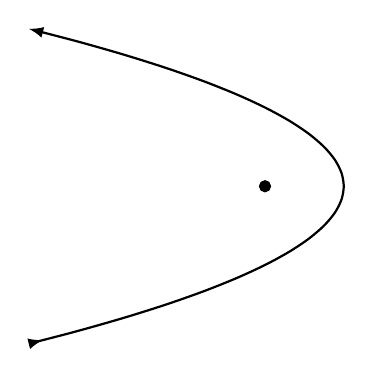
\begin{tikzpicture}[>=latex]

        \draw[scale=1,domain=-2:2,smooth,variable=\t, >->, thick] plot ({-(\t)^2+1},\t);
        \filldraw[] (0,0) circle (2pt);

    \end{tikzpicture}
    \caption{A parabolic trajectory}\label{fig:Parabolic Trajectory}
\end{figure}

The eccentricity of a parabola is, by definition, $e=1$. It is also proven in Section \ref{sec:Kepler's First Law} that when $e=1$ the orbit equation creates a parabola. For the numerator of the orbit equation $r=\frac{a(1-e^2)}{1+e\cos(\theta)}$ to be nonzero, $a$ must be infinite. The velocity in a parabolic orbit can be investigated with Equation \eqref{Vis-Viva Equation}.

\begin{align*}
    v & =\sqrt{\frac{2\mu}{r}-\frac{\mu}{a}}                                                     \\
      & =\sqrt{\frac{2\mu}{r}-\lim_{a\rightarrow\infty}\left(\frac{\mu}{a}\right)}               \\
      & =\sqrt{\frac{2\mu}{r}-\cancelto{0}{\lim_{a\rightarrow\infty}\left(\frac{\mu}{a}\right)}} \\
\end{align*}
\begin{equation}
    v_\text{parabola}=v_\text{esc}=\sqrt{\frac{2\mu}{r}}
\end{equation}

Since a parabola has a determined unique shape, there is only one parameter for it; its size. The defining parameter for a parabolic trajectory is either the periapsis $r_\text{pe}$ or the semi-latus rectum $p$, which can be related using Equation \eqref{Polar with p, e} keeping in mind that at periapsis the cosine will evaluate to 1
\begin{align*}
    r           & =\frac{p}{1+e\cos(\theta-\omega)} \\
    r_\text{pe} & =\frac{p}{1+\cos(0)}              \\
    r_\text{pe} & =\frac{p}{2}                      \\
\end{align*}
\begin{equation}
    p_\text{parabola}=2r_\text{pe,parabola}
\end{equation}

To determine the periapsis of a parabolic trajectory from a measured velocity, angular momentum must be used

\begin{align*}
    h_\text{pe}            & = h                                                   \\
    r_\text{pe}v_\text{pe} & =rv\cos(\phi)                                         \\
    r_\text{pe}            & =\frac{rv\cos(\phi)}{v_\text{pe}}                     \\
                           & =\frac{rv\cos(\phi)}{\sqrt{\frac{2\mu}{r_\text{pe}}}} \\
    r_\text{pe}^2          & =\frac{r^2v^2\cos^2(\phi)}{\frac{2\mu}{r_\text{pe}}}  \\
    r_\text{pe}^2          & =\frac{r_\text{pe}r^2v^2\cos^2(\phi)}{2\mu}           \\
\end{align*}
\begin{equation}\label{Periapsis Radius Parabola}
    r_\text{pe,parabola}=\frac{r^2v^2\cos^2(\phi)}{2\mu}
\end{equation}

\bigskip\bigskip
\subsection{Conclusion}

\bigskip
Hyperbolic orbits approach a linear trajectory with an angle of
$$\theta_\text{hyp}=\arctan\left(\sqrt{e^2-1}\right)$$

\bigskip
Because hyperbolas don't have physically meaningful apoapses, the semi-major axis and eccentricity can be defined in terms of the entry/exit angle $\theta_\text{hyp}$ and the periapsis radius $r_\text{pe}$.
$$e=\sec(\theta_\text{hyp})\qquad\qquad a=\frac{{r_\text{pe}}}{1-\sec(\theta_\text{hyp})}$$

\bigskip
Parabolic trajectories occur at exactly escape velocity, meaning that at all points
$$v=\sqrt{\frac{2\mu}{r}}$$

\bigskip
In a parabolic trajectory, the semi-latus rectum and periapsis are related by
$$p_\text{parabola}=2r_\text{pe,parabola}$$

\bigskip
From telemetry data, the periapsis radius can be found with
$$r_\text{pe,parabola}=\frac{r^2v^2\cos^2(\phi)}{2\mu}$$

\pagebreak
\section{Orbital Manuevers Basics}

Throughout this section, burns are assumed to be pseudo-impulsive. That is to say, they occur over an infinitesimal amount of distance and time. The $n$ vectors can change throughout the burn (and in fact, they do) with change in direction of velocity. It is assumed for ease of analysis that the spacecraft's thrust vector shifts to keep up with the $m$ vectors. It is important to remember that the $m$ vectors are based on velocity, not on position. That is to say, $\hat{m}_r$ does not necessarily point outward from the planet, but rather it points perpendicular to the velocity vector and in plane with the orbit. Only at the apses does $\hat{m}_v$ point perpendicular to the displacement from the planet. Similarly, only at the apses does $\hat{m}_r$ point radially outward from the planet.

\bigskip\bigskip
\subsection{Rocket Equation}

The rocket equation describes the relationship between the obtained change in velocity $\Delta{}v$ is related to the change in mass of a spacecraft.

\begin{figure}[H]
    \centering
    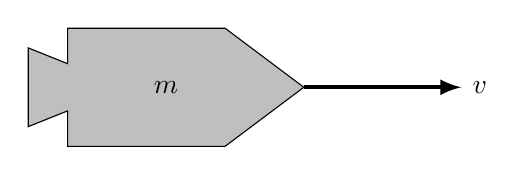
\begin{tikzpicture}[>=latex]
        \filldraw[lightgray, draw=black] (3.5,0)--(2.5,.75)--(0.5,.75)--(0.5,0.3)--(0,0.5)--(0,0)--(0,-0.5)--(0.5,-0.3)--(0.5,-.75)--(2.5,-.75)--cycle;
        \draw[ultra thick, ->] (3.5,0)--+(2,0) node[right] {$v$};
        %\draw[ultra thick, ->] (-1,0)--+(-2,0) node[left] {$v_e$};
        %\node[circle, fill=white, draw=gray] at (-1,0) {$m_e$};
        \node[] at (1.75,0) {$m$};
    \end{tikzpicture}

    \bigskip

    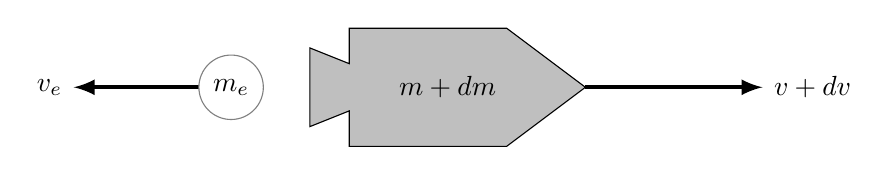
\begin{tikzpicture}[>=latex]
        \filldraw[lightgray, draw=black] (3.5,0)--(2.5,.75)--(0.5,.75)--(0.5,0.3)--(0,0.5)--(0,0)--(0,-0.5)--(0.5,-0.3)--(0.5,-.75)--(2.5,-.75)--cycle;
        \draw[ultra thick, ->] (3.5,0)--+(2.25,0) node[right] {$v+dv$};
        \draw[ultra thick, ->] (-1,0)--+(-2,0) node[left] {$v_e$};
        \node[circle, fill=white, draw=gray] at (-1,0) {$m_e$};
        \node[] at (1.75,0) {$m+dm$};
    \end{tikzpicture}

    \caption{A spacecraft with some exhaust exiting it}
\end{figure}

First, conservation of energy will be applied. For mass to be conserved, $m_e=-dm$.
\begin{align*}
    p_1                & =p_2                                                  \\
    p_\text{rocket,1}  & =p_\text{rocket,2}+p_\text{exhaust}                   \\
    mv                 & =(m+dm)(v+dv)+m_e(v-v_e)                              \\
    mv                 & =(m+dm)(v+dv)-dm(v-v_e)                               \\
    mv                 & =mv+mdv+vdm+dmdv-vdm+v_edm                            \\
    \cancel{mv}        & =\cancel{mv}+mdv+\cancel{vdm}+dmdv-\cancel{vdm}+v_edm \\
    0                  & =mdv+dmdv+v_edm                                       \\
                       & \text{The second-order differential $dmdv$ vanishes}  \\
    0                  & =mdv+v_edm                                            \\
    -mdv               & =v_edm                                                \\
    dv                 & =\frac{-v_edm}{m}                                     \\
    \int_{v_1}^{v_2}dv & =-v_e\int_{m_1}^{m_2}\frac{1}{m}dm                    \\
    \Delta{}v          & =-v_e(\ln(m_2)-\ln(m_1))                              \\
    \Delta{}v          & =-v_e\ln(\frac{m_2}{m_1})                             \\
\end{align*}

\begin{equation}\label{Rocket Equation Ve}
    \Delta{}v=v_e\ln\left(\frac{m_1}{m_2}\right)
\end{equation}

This equation has another (equivalent) form. Because exhaust velocity can come in many different units, making it hard to compare between spacecraft. Instead of the exhaust velocity, a specific impulse $I_sp$ is defined. The specific impulse is the exhaust velocity divided by Earth's standard gravity at sea level. This allows the units to cancel out to seconds. $I_{sp}=\frac{v_e}{g_0}\rightarrow{}v_e=I_{sp}g_0$

\begin{equation}\label{Rocket Equation ISP}
    \Delta{}v=I_{sp}g_0\ln\left(\frac{m_1}{m_2}\right)
\end{equation}

Note that $\Delta v$ is not actually the change in velocity; a spacecraft can burn for a change in velocity of some arbitrary amount $\delta$ in one direction, then perform a burn of equal magnitude in a perpendicular direction. The magnitude of the change in velocity of the spacecraft is $\sqrt{2}\delta$, while the change in magnitude of velocity would depend on the initial velocity vector of the spacecraft. Instead, $\Delta v$ can be treated as a quantity that a spacecraft expends as it performs manuevers. For the rest of this chapter, the uppercase $\Delta V$ will be used to make this distinction, with the differential form $dV$ being used as well. Keep in mind that, while $dV$ and $\Delta V$ have units of velocity, they are \textit{not} necessarily equal to differential or absolute changes in the actual magnitude of velocity. When $dV$ is integrated, the integration bounds will be $V$- think of this as the currency which is being used, or a means of measuring fuel requirements for maneuvers.

\bigskip\bigskip
\subsection{Burns in the \texorpdfstring{$\hat{m}_r$}{Radial} Direction}\label{sec:Mr manuevers}

\begin{figure}[H]
    \centering
    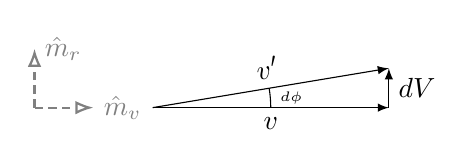
\begin{tikzpicture}[>=latex]
        \def\vel{3}
        \def\dV{0.5}
        \def\velLong{\fpeval{sqrt(\vel^2+\dV^2)}}
        \def\dPhi{\fpeval{atan(\dV/\vel)}}
        \def\arcRad{1.5}
        \def\unMag{0.75}

        \draw[->] (0,0) -- +({deg(\dPhi)}:\velLong) node[midway,sloped,above] {$v'$};
        \draw[->] (0,0) -- +(\vel,0) node[midway,below] {$v$};
        \draw[->] (\vel,0) -- +(0,\dV) node[midway,right] {$dV$};
        \draw[] (\arcRad,0) arc (0:{deg(\dPhi)}:\arcRad) node[midway, right] {\tiny $d\phi$};

        \draw[densely dashed, -{Latex[open]}, gray, thick] (-1.5,0) -- +(90:\unMag) node[right] {$\hat{m}_r$};
        \draw[densely dashed, -{Latex[open]}, gray, thick] (-1.5,0) -- +(0:\unMag) node[right] {$\hat{m}_v$};
    \end{tikzpicture}
    \caption{Velocity change due to thrust in the $\hat{m}_r$ direction}\label{fig:dV Triangle Mr}
\end{figure}

It can be shown that $v'=v$.

\begin{align*}
    v'     & = \sqrt{v^2+dV^2}                                        \\
    (v')^2 & = v^2+dV^2                                               \\
    (v')^2 & = v^2+\cancelto{\text{smaller order differential}}{dV^2} \\
    (v')^2 & = v^2                                                    \\
    v'     & = v                                                      \\
\end{align*}

This proves that, when $dV$ is always perpendicular to the velocity vector, there is no change in magnitude of velocity. Because the magnitude of velocity is conserved, Equation \eqref{Specific Energy Physical} implies that specific energy is conserved. Equation \eqref{Specific Energy Geometric} shows that the semi-major axis is also unchanged due to the conservation of specific energy.

However, the flight path angle $\phi$ does change. Remember throughout this process that $v$ is constant.

\begin{align*}
    dV                     & =vd\phi                         \\
    d\phi                  & = \frac{dV}{v}                  \\
    \int_{\phi_1}^{\phi_2} & = \frac{1}{v}\int_{V_1}^{V_2}dV \\
    \Delta \phi            & = \frac{\Delta V}{v}            \\
\end{align*}

While the magnitude of velocity is not changed, its direction relative to the $u$ vectors (and any inertial base frame) is changed. Equation \eqref{Flight Path Angle} shows the relationship between $\phi$ and geometric parameters of the orbit.
$$\cos(\phi)=\sqrt{\frac{a^2(1-e^2)}{r(2a-r)}}$$

Because $a$ and $r$ are unchanged, $e$ must change. The precise change in $e$ can be investigated by solving for $e_2$, the eccentricity of the orbit post-burn.

\begin{align*}
    \sqrt{\frac{a^2(1-e_2^2)}{r(2a-r)}}                                   & =\cos(\phi+\Delta \phi)                                                                                                 \\
                                                                          & =\cos(\phi)\cos(\Delta \phi)-\sin(\phi)\sin(\Delta \phi)                                                                \\
                                                                          & =\cos(\phi)\cos(\Delta \phi)-\sqrt{1-\cos^2(\phi)}\sin(\Delta \phi)                                                     \\
                                                                          & =\sqrt{\frac{a^2(1-e^2)}{r(2a-r)}}\cos(\Delta \phi)-\sqrt{1-\frac{a^2(1-e^2)}{r(2a-r)}}\sin(\Delta \phi)                \\
    \sqrt{\frac{a^2(1-e_2^2)}{r(2a-r)}}/\sqrt{\frac{a^2(1-e^2)}{r(2a-r)}} & =\cos(\Delta \phi)-\frac{\sqrt{1-\frac{a^2(1-e^2)}{r(2a-r)}}}{\sqrt{\frac{a^2(1-e^2)}{r(2a-r)}}}\sin(\Delta \phi)       \\
    \sqrt{\frac{a^2(1-e_2^2)}{a^2(1-e^2)}}                                & =\cos(\Delta \phi)-\frac{\sqrt{\frac{r(2a-r)-a^2(1-e^2)}{r(2a-r)}}}{\sqrt{\frac{a^2(1-e^2)}{r(2a-r)}}}\sin(\Delta \phi) \\
    \sqrt{\frac{1-e_2^2}{1-e^2}}                                          & =\cos(\Delta \phi)-\sqrt{\frac{\frac{r(2a-r)-a^2(1-e^2)}{r(2a-r)}}{\frac{a^2(1-e^2)}{r(2a-r)}}}\sin(\Delta \phi)        \\
    \sqrt{\frac{1-e_2^2}{1-e^2}}                                          & =\cos(\Delta \phi)-\sqrt{\frac{r(2a-r)-a^2(1-e^2)}{a^2(1-e^2)}}\sin(\Delta \phi)                                        \\
    \sqrt{\frac{1-e_2^2}{1-e^2}}                                          & =\cos(\Delta \phi)-\sqrt{\frac{r(2a-r)}{a^2(1-e^2)}-1}\sin(\Delta \phi)                                                 \\
    \sqrt{\frac{1-e_2^2}{1-e^2}}                                          & =\cos(\Delta \phi)-\sqrt{1/\left(\sqrt{\frac{a^2(1-e^2)}{r(2a-r)}}\right)^2-1}\sin(\Delta \phi)                         \\
    \sqrt{\frac{1-e_2^2}{1-e^2}}                                          & =\cos(\Delta \phi)-\sqrt{\frac{1}{\cos^2(\phi)}-1}\sin(\Delta \phi)                                                     \\
    \sqrt{\frac{1-e_2^2}{1-e^2}}                                          & =\cos(\Delta \phi)-\sqrt{\sec^2(\phi)-1}\sin(\Delta \phi)                                                               \\
    \sqrt{\frac{1-e_2^2}{1-e^2}}                                          & =\cos(\Delta \phi)-\sqrt{\tan^2(\phi)}\sin(\Delta \phi)                                                                 \\
    \sqrt{\frac{1-e_2^2}{1-e^2}}                                          & =\cos(\Delta \phi)-\tan(\phi)\sin(\Delta \phi)                                                                          \\
    \frac{1-e_2^2}{1-e^2}                                                 & =(\cos(\Delta \phi)-\tan(\phi)\sin(\Delta \phi))^2                                                                      \\
    1-e_2^2                                                               & =(\cos(\Delta \phi)-\tan(\phi)\sin(\Delta\phi))^2(1-e^2)                                                                \\
    e_2^2                                                                 & =1-(\cos(\Delta \phi)-\tan(\phi)\sin(\Delta\phi))^2(1-e^2)                                                              \\
    e_2^2                                                                 & =1-\Bigl(\cos^2(\Delta\phi)+\tan^2(\phi)\sin^2(\Delta\phi)-\tan(\phi)\sin(\Delta\phi)\cos(\Delta\phi)\Bigr)(1-e^2)      \\
    e_2^2                                                                 & =1-\cos^2(\Delta\phi)\Bigl(1+\tan^2(\phi)\tan^2(\Delta\phi)-\tan(\phi)\tan(\Delta\phi)\Bigr)(1-e^2)                     \\
    e_2^2                                                                 & =1-\cos^2(\Delta\phi)\Bigl(1-\tan(\phi)\tan(\Delta\phi)\Bigr)^2(1-e^2)                                                  \\
    e_2                                                                   & =\sqrt{1-(1-e^2)\cos^2(\Delta\phi)\Bigl(1-\tan(\phi)\tan(\Delta\phi)\Bigr)^2}
\end{align*}
\begin{equation*}
    e_2=\sqrt{1-(1-e^2)\cos^2\left(\frac{\Delta V}{v}\right)\left(1-\tan(\phi)\tan\left(\frac{\Delta V}{v}\right)\right)^2}
\end{equation*}

This formula is here for the sake of completeness, however in it is utterly useless for analysis.

Recall that $\phi$ is constrained $\frac{-\pi}{2}<\phi<\frac{\pi}{2}$ (at $\phi=\pm\frac{\pi}{2}$, $\hat{m}_r$ is undefined as there are infinitely many vectors normal to velocity and in plane with the displacement vector). Any thrust in the $\hat{m}_r$ direction will increase $\phi$.

The following equation will be analyzed to determine how manuevers in $\hat{m}_r$ impact $e$.
$$\cos(\phi)=\sqrt{\frac{a^2(1-e^2)}{r(2a-r)}}$$

As $\phi$ increases within the domain $\frac{-\pi}{2}<\phi<0$, $\cos(\phi)$ increases, meaning that $1-e^2$ must increase as well, so $e$ must decrease. On the domain $0<\phi<\frac{\pi}{2}$, the opposite holds true; increase in $\phi$ means an increase in $e$. When $\phi$ is negative, the spacecraft's distance to the planet is decreasing. This means that the spacecraft is approaching periapsis. When $\phi$ is positive, the spacecraft is approaching apoapsis.

From Equation \eqref{True Anomoly Geometric}, an increase in eccentricity will increase the angle to the periapsis, while a decrease in eccentricity will decrease the angle to periapsis.

This means that if the spacecraft is heading towards periapsis, a radial out burn (by decreasing eccentricity) will bring the periapsis up and closer to the spacecraft's true anomaly. When the spacecraft is heading towards apoapsis, a radial out burn will (by increasing efficiency) further raise the apoapsis while increasing the angle to periapsis and therefore decreasing the angle to apoapsis.
%TODO: UNCOMMENT
\begin{comment}
\begin{figure}[H]
    \centering
    \begin{tikzpicture}[>=latex]
        \def\SMA{2}
        \def\vO{7}
        \def\phiO{0}
        \def\X{\fpeval{-sqrt(3)}}
        \def\Y{1}
        \def\posR{\fpeval{sqrt((\X)^2+\Y^2)}}
        \fill(0,0) circle (2pt);
        \foreach \dV in {1,2,3,4,5,6,7,8,9,10}
        {
        \definecolor{orbCol}{gray}{\fpeval{1-\dV/20}}
        \def\ecc{\fpeval{sqrt(1-(cos(\dV/\vO))^2*(1-tan(\phiO)*tan(\dV/\vO))^2)}}
        \def\omeg{\fpeval{atan(\Y/\X)-acos((\SMA*(1-\ecc^2)-\posR)/(\ecc*\posR))}}
        \def\slr{\fpeval{\SMA*(1-\ecc^2)}}
        \draw[domain=0:2*pi,samples=300, orbCol] plot ({deg(\x+\omeg)-180}:{(\slr)/(1+\ecc*cos(\x r))});
        \fill[blue] (\X,\Y) circle (3pt);
        }
    \end{tikzpicture}
    \caption{A counterclockwise orbit with progressively-labeled burns in the $\hat{u}_r$ direction. The darker the orbit, the more $\Delta V$ has been expended. The beginning orbit is the near-circular one. The spacecraft is the blue point. If the spacecraft were instead orbiting clockwise, then the lighter shades would indicate more $\Delta V$ expenditure with the darker orbit being the original orbit}
\end{figure}
\end{comment}

Conclusion: any burn in the $\hat{m}_r$ direction raises apsis that the spacecraft is approaching while lowering the apsis that the spacecraft is coming from. The orbit "pivots" about the spacecraft, with the eccentricity changing and the semi-major axis remaining the same. The increase in one apsis is equal to the decrease in the other apsis (see Figure \ref{fig:Orbit Diagram}). The true anomaly of whichever apsis the spacecraft is heading towards will be brought closer to the spacecraft. Because the plane of the orbit is unchanged, $\Omega$ and $i$ are kept the same with radial manuevers. To keep the spacecraft where it is, $\omega+\theta$ is also not changed.

Radial in burns are the reverse of radial out burns.

\bigskip\bigskip
\subsection{Burns in the \texorpdfstring{$\hat{m}_n$}{Normal} Direction}\label{sec:Mn Manuever}

\begin{figure}[H]
    \centering
    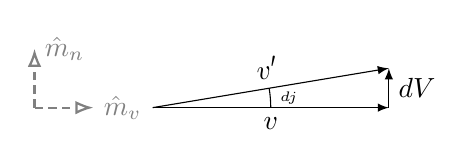
\begin{tikzpicture}[>=latex]
        \def\vel{3}
        \def\dV{0.5}
        \def\velLong{\fpeval{sqrt(\vel^2+\dV^2)}}
        \def\dPhi{\fpeval{atan(\dV/\vel)}}
        \def\arcRad{1.5}
        \def\unMag{0.75}

        \draw[->] (0,0) -- +({deg(\dPhi)}:\velLong) node[midway,above,sloped] {$v'$};
        \draw[->] (0,0) -- +(\vel,0) node[midway,below] {$v$};
        \draw[->] (\vel,0) -- +(0,\dV) node[midway,right] {$dV$};
        \draw[] (\arcRad,0) arc (0:{deg(\dPhi)}:\arcRad) node[midway, right] {\tiny $dj$};

        \draw[densely dashed, -{Latex[open]}, gray, thick] (-1.5,0) -- +(90:\unMag) node[right] {$\hat{m}_n$};
        \draw[densely dashed, -{Latex[open]}, gray, thick] (-1.5,0) -- +(0:\unMag) node[right] {$\hat{m}_v$};
    \end{tikzpicture}
    \caption{Velocity change due to thrust in the $\hat{m}_n$ direction}\label{fig:dV Triangle Mn}
\end{figure}

Much like in Section \ref{sec:Mr manuevers}, the magnitude of velocity does not change. Instead of $\phi$ changing, the inclination of the orbit changes. Note that instead of using $i$, $j$ is used here. This is because $\Delta V$ causes a linear change in the angle between the planes of the pre-burn and post-burn orbits. However, the inclination measures the angle between the post-burn orbit and some arbitrary horizon. $\Delta j$ is very easy to find, with $\Delta i$ requiring some geometric reasoning.

Using the same mathematics as in Section \ref{sec:Mr manuevers}, it is apparent that $\Delta j=\frac{\Delta V}{v}$.

This means that normal burns have the effect of "tilting" the plane of the orbit about the line connecting the spacecraft and the orbited body. The two points at which the orbit intersects the reference plane are the ascending and descending nodes. At the ascending node, the spacecraft goes from negative latitude to positive latitude. At the descending node, it goes from positive latitude to negative latitude.

\begin{figure}[H]
    \centering
    \def\ecc{0}
    \def\SMA{3}
    \def\incI{20}
    \def\dJ{20}

    \tdplotsetmaincoords{70}{30}
    \begin{tikzpicture}[tdplot_main_coords, >=latex]

        \tdplotsetrotatedcoords{0}{-\dJ}{0}

        % post-burn orbit
        \draw[tdplot_rotated_coords, blue, samples=250] plot ({deg(\x)}:\SMA);
        \draw[tdplot_rotated_coords,blue, ->] (0,0,0) -- +(\SMA,0,0);
        \draw[tdplot_rotated_coords,blue, ->] (0,0,0) -- +(0,0,1);

        %original orbit
        \draw[lightgray, samples=250, red] plot ({deg(\x)}:\SMA);
        \draw[red, ->] (0,0,0) -- +(\SMA,0,0);
        \draw[red, ->] (0,0,0) -- +(0,0,1);

        % Axis of rotation
        \filldraw[] (0,-\SMA,0) circle (2pt);
        \draw[densely dashed] (0,\SMA,0)--(0,-\SMA,0);

        % inclination labels
        \draw[tdplot_rotated_coords,gray, densely dashed] (0,0,0) -- +(0,0,2);
        \draw[densely dashed, gray] (0,0,0) -- (0,0,2);
        \tdplotsetrotatedcoords{-90}{90}{90}
        \draw[tdplot_rotated_coords, densely dashed, thick] (0,2,0) arc (90:90+\dJ:2) node[midway, above] {$\Delta j$};

        \draw[tdplot_rotated_coords, densely dashed, thick] (\SMA,0, 0) arc (0:\dJ:\SMA) node[midway, right] {$\Delta j$};
    \end{tikzpicture}

    \caption{A manuever in the $\hat{m}_n$ direction performed at position indicated by the black dot}\label{fig:Inclination Changes}
\end{figure}

If the original orbit (red) is inclined by some angle $i$ in such a way that $i$ and $\Delta j$ are not in the same direction, finding the change in inclination is not simple addition. If $\Delta j$ is not in the same direction as $i$, $\Delta i \ne \Delta j$, and the longitude of ascending node $\Omega$ will be changed.

It will now become useful to express inclination as a vector. A normal burn has the effect of adding another inclination vector to the original inclination vector. The inclination is a rotation of the orbit about a vector that points from the orbited body to the ascending node.

The inclination can be expressed as a rotation of $i\hat{b}_1$ (see Appendix Figure \ref{fig:Frames}). A burn in the $\hat{m}_n$ direction will cause a rotation of $\Delta j\hat{u}_r$ vector. Therefore,
$$i_2=|i\hat{b}_1+\Delta j\hat{u}_r|$$

Conclusion: normal burns rotate the orbit about the polar $\hat{u}_r$ vector.

\bigskip\bigskip
\subsection{Burns in the \texorpdfstring{$\hat{m}_v$}{Velocity} Direction}

Returning once more to the simple realm of in-plane orbits, a burn in the $\hat{m}_v$ direction carries the unique property that $\Delta V$ actually \textit{is} in the direction of velocity, meaning $\Delta V$ is equal to the change in magnitude of velocity and the magnitude of change in velocity. This means that
$$v_2=v+\Delta v$$

Using Equation \eqref{Specific Energy Physical}, the change in specific energy can be found.

\begin{align*}
    \Delta \varepsilon & = \varepsilon_2 - \varepsilon                                                                        \\
                       & = \left(\frac{(v+\Delta V)^2}{2}-\frac{\mu{}}{r}\right) - \left(\frac{v^2}{2}-\frac{\mu{}}{r}\right) \\
                       & = \frac{1}{2}\left(\left(v+\Delta V\right)^2-v^2\right)                                              \\
                       & = \frac{1}{2}\left(\left(v^2+(\Delta V)^2+v\Delta V\right)-v^2\right)                                \\
                       & = \frac{1}{2}\left((\Delta V)^2+v\Delta V\right)                                                     \\
                       & = \frac{1}{2}\Delta V\left(\Delta V+v\right)                                                         \\
\end{align*}

This means that, to maximize specific energy gained for any given $\Delta V$, a burn should be done when the spacecraft is at its maximum speed, which occurs at Periapsis.

Because $\varepsilon$ changes, Equation \eqref{Specific Energy Geometric} implies that the semi-major axis changes as well.

\begin{align*}
    \varepsilon & = \frac{-\mu}{2a}           \\
    a           & = \frac{-\mu}{2\varepsilon} \\
\end{align*}

The proportional change in $a$ will be found. That is to say, the ratio of $a_2$ and $a$.

\begin{align*}
    \frac{a_2}{a} & = (\frac{-\mu}{2\varepsilon})/(\frac{-\mu}{2(\varepsilon+\frac{1}{2}\Delta V\left(\Delta V+v\right))})         \\
                  & = \left(\frac{-\mu}{2\varepsilon}\right)/\left(\frac{-\mu}{\varepsilon+\Delta V\left(\Delta V+v\right)}\right) \\
                  & = \frac{\varepsilon+\Delta V\left(\Delta V+v\right)}{2\varepsilon}                                             \\
                  & = 1+\frac{\Delta V\left(\Delta V+v\right)}{2\varepsilon}                                                       \\
                  & = 1+\frac{\Delta V\left(\Delta V+v\right)}{2\left(\frac{v^2}{2}-\frac{\mu{}}{r}\right)}                        \\
                  & = 1+\frac{\Delta V\left(\Delta V+v\right)}{v^2-\frac{2\mu{}}{r}}                                               \\
\end{align*}

However, a more simple means of finding $\Delta a$ can be found using Equation \eqref{Vis-Viva Equation}.

\begin{align*}
    v + \Delta V                            & = \sqrt{\frac{2\mu}{r}-\frac{\mu}{a_2}}                        \\
    (v + \Delta V)^2                        & = \left(\sqrt{\frac{2\mu}{r}-\frac{\mu}{a_2}}\right)^2         \\
    v^2 + (\Delta V)^2 + 2v\Delta V         & = \frac{2\mu}{r}-\frac{\mu}{a_2}                               \\
    \frac{v^2+(\Delta V)^2+2v\Delta V}{\mu} & =\frac{2}{r}-\frac{1}{a_2}                                     \\
    \frac{1}{a_2}                           & =\frac{2}{r}-\frac{v^2+(\Delta V)^2+2v\Delta V}{\mu}           \\
    \frac{1}{a_2}                           & =\frac{2\mu}{r\mu}-\frac{rv^2+r(\Delta V)^2+2rv\Delta V}{r\mu} \\
    \frac{1}{a_2}                           & =\frac{2\mu-rv^2-r(\Delta V)^2-2rv\Delta V}{r\mu}              \\
    {a_2}                                   & =\frac{r\mu}{2\mu-rv^2-r(\Delta V)^2-2rv\Delta V}              \\
\end{align*}

Conclusion: burns in the $\hat{m}_v$ direction increase the semi-major axis of the orbit. Because the point that the spacecraft occupies must remain fixed, the opposite side of the orbit exhibits the most change in radius.

\subsection{Conclusion}

\bigskip
The rocket equation describes the change in velocity (or, more accurately, the magnitude of the vector change in velocity) due to the expendature of propellant in a spacecraft. Because all maneuvers require changing velocity, this $\Delta V$ is treated as a means of measuring mission requirements, almost like a fuel requirement.
$$\Delta V = I_{sp}g_0\ln\left(\frac{m_1}{m_2}\right)$$

\bigskip
If a spacecraft burns radially outward (that is to say, perpendicular from and in plane with its velocity and generally away from the planet), this will have the effect of raising the next apsis and lowering the opposite one, while bringing the next apsis closer to the spacecraft's position. This will change the eccentricity of the orbit.

Out-of-plane burns change the inclination of an orbit about the point at which the maneuver is performed. Because the plane of the orbit is defined by the velocity vector and the radial vector, knowledge of the direction of the velocity vector and radial vector allow the plane of the orbit to be known.

Burns along the velocity vector increase the semi-major axis by raising the opposite side of the orbit, while burns opposite the velocity vector have the opposite effect.

\pagebreak
\section{Practical Maneuvers}

\bigskip\bigskip
\subsection{Inclination Change}

In Section \ref{sec:Mn Manuever}, maneuvers were done at a constant angle to the velocity vector. However, it is more efficient to transfer to the desired orbit directly by finding the vector difference between the old velocity and the desired velocity. To maximize the effect of such a manuever, it should be done at either the ascending or descending node (such that $\Delta j=\Delta i$).

\begin{figure}[H]
    \centering
    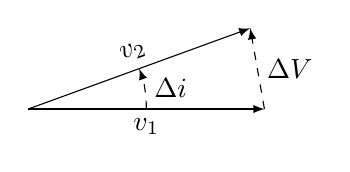
\begin{tikzpicture}[>=latex]
        \def\vel{3}
        \def\dPhi{20}
        \def\arcRad{1.5}

        \draw[->] (0,0) -- +(\dPhi:\vel) node[midway,above,sloped] {$v_2$};
        \draw[->] (0,0) -- +(\vel,0) node[midway,below] {$v_1$};
        \draw[dashed, ->] (\vel,0) -- (\dPhi:\vel) node[midway,right] {$\Delta V$};
        \draw[dashed, ->] (\arcRad,0) arc (0:\dPhi:\arcRad) node[midway, right] {$\Delta i$};
    \end{tikzpicture}
    \caption{Inclination change velocity}\label{fig:dV Triangle Inclination Chage}
\end{figure}

Because the only effect of this maneuver is to change the direction of velocity, $\Delta V$ is the magnitude of the vector difference in the old velocity and the new velocity. Note that, throughout this maneuver, the magnitude of velocity will first decrease and then increase, so there is no net effect on the shape of the orbit in its own plane.

\begin{align*}
    \Delta V & = |\vv{v}_2-\vv{v}_1|                                                    \\
             & = |(v\cos(\Delta i)\hat{m}_v+v\sin(\Delta i)\hat{m}_n)-(v\hat{m}_v)|     \\
             & = |v(\cos(\Delta i)-1)\hat{m}_v+v\sin(\Delta i)\hat{m}_n|                \\
             & = \sqrt{(v(\cos(\Delta i)-1))^2+(v\sin(\Delta i))^2}                     \\
             & = \sqrt{v^2(\cos(\Delta i)-1)^2+v^2\sin^2(\Delta i)}                     \\
             & = v\sqrt{(\cos(\Delta i)-1)^2+\sin^2(\Delta i)}                          \\
             & = v\sqrt{\cos^2(\Delta i)+1-2\cos(\Delta i)+\sin^2(\Delta i)}            \\
             & = v\sqrt{(\cos^2(\Delta i)+\cos^2(\Delta i))+1-2\cos(\Delta i)}          \\
             & = v\sqrt{2-2\cos(\Delta i)}                                              \\
             & = v\sqrt{2(1-\cos(\Delta i))}                                            \\
             & = v\sqrt{2\left(1-\cos\left(2\frac{\Delta i}{2}\right)\right)}           \\
             & = v\sqrt{4\left(\frac{1-\cos\left(2\frac{\Delta i}{2}\right)}{2}\right)} \\
             & = v\sqrt{4\sin^2\left(\frac{\Delta i}{2}\right)}                         \\
\end{align*}

This gives us the $\Delta V$ required for an inclination change maneuver
\begin{equation}
    \Delta V= 2\sin\left(\frac{\Delta i}{2}\right)
\end{equation}

This shows the minimum required $\Delta V$ for an orbital inclination change. If the inclination change occurs at any point other than the ascending or descending node, it will require a greater $\Delta V$ and will also have the effect of chaning the longitude of ascending node $\Omega$ (and therefore moving the ascending and descending nodes). In-plane maneuvers will change neither the inclination nor the longitude of ascending node.

\bigskip\bigskip
\subsection{Hohmann Transfer}

A Hohmann Transfer is a transfer between two circular orbits from radius $r_1$ to radius $r_2$. The transfer is done via an elliptical orbit, and takes two burns. The first burn puts the orbit into an elliptical orbit in which the periapsis is the lower orbit, and the apoapsis is the higher orbit. The second burn transfers from the elliptic orbit into the final circular orbit.

\begin{figure}[H]
    \centering
    \def\Rone{0.75}
    \def\Rtwo{2.5}
    \def\transSMA{\fpeval{(\Rone+\Rtwo)/2}}
    \def\ctrX{\fpeval{\Rone-\transSMA}}
    \def\trE{\fpeval{\Rtwo/\transSMA - 1}}
    \def\transSmA{\fpeval{\transSMA*sqrt(1-(\trE)^2)}}
    \def\dV{1.25}
    \definecolor{purp}{rgb}{.8,0,.8}
    \begin{tikzpicture}[>=latex]
        \draw[thin, dotted, blue] (0,0) ellipse ({\Rone} and {\Rone});
        \draw[blue, thick,>-] (-\Rone,0) arc (180:360:{\Rone} and {\Rone}) node[right] {$r_1$};


        \draw[thin, dotted, purp] (\ctrX,0) ellipse ({\transSMA} and {\transSmA});
        \draw[purp, thick] (\Rone,0) arc (0:180:{\transSMA} and {\transSmA});

        \draw[thin, dotted,red] (0,0) ellipse ({\Rtwo} and {\Rtwo});
        \draw[red, thick,->] (-\Rtwo,0) arc (180:360:{\Rtwo} and {\Rtwo}) node[right] {$r_2$};;

        \filldraw[lightgray] (0,0) circle (2pt);

        \draw[->] (\Rone,0)--+(0,\dV) node[above] {$\Delta v_1$};
        \draw[->] (-\Rtwo,0)--+(0,-\dV) node[below] {$\Delta v_2$};

    \end{tikzpicture}
    \begin{tikzpicture}[>=latex]
        \draw[->] (\Rone,0)--+(0,-\dV) node[below] {$\Delta v_1$};
        \draw[->] (-\Rtwo,0)--+(0,\dV) node[above] {$\Delta v_2$};

        \draw[thin, dotted, red] (0,0) ellipse ({\Rone} and {\Rone});
        \draw[red, thick,->] (\Rone,0) arc (0:180:{\Rone} and {\Rone}) node[left] {$r_2$};


        \draw[thin, dotted, purp] (\ctrX,0) ellipse ({\transSMA} and {\transSmA});
        \draw[purp, thick] (-\Rtwo,0) arc (180:360:{\transSMA} and {\transSmA});

        \draw[thin, dotted,blue] (0,0) ellipse ({\Rtwo} and {\Rtwo});
        \draw[blue, thick,>-] (\Rtwo,0) arc (0:180:{\Rtwo} and {\Rtwo}) node[left] {$r_1$};;

        \filldraw[lightgray] (0,0) circle (2pt);

    \end{tikzpicture}
    \caption{A Hohmann Transfer from a low orbit to a high orbit (left) and from a high orbit to a lower one (right)}\label{fig:Hohmann Transfer}
\end{figure}

Because both burns are along the velocity vector, $\Delta V=\Delta v_1+\Delta v_2$. $a_1=r_1=r_\text{pe,tr}$ will refer to the semi-major axis of the smaller orbit, with $a_2=r_2=r_\text{ap,tr}$ being the semi-major axis of the larger orbit. The semi-major axis of the transfer orbit is $a_\text{tr}=\frac{1}{2}(r_1+r_2)$. $v_1$ and $v_2$ refer to the circular orbit velocities in the original and new orbit. The below calculations assume a transfer from a low orbit into a higher one.

\begin{align*}
    \Delta V & = \Delta v_1+\Delta v_2                                                                                                                                                                                                           \\
             & = (v_\text{pe,tr}-v_1)+(v_2-v_\text{ap,tr})                                                                                                                                                                                       \\
             & = \left(\sqrt{\frac{2\mu}{r_\text{pe,tr}}-\frac{\mu}{a_\text{tr}}}-\sqrt{\frac{2\mu}{r_1}-\frac{\mu}{a_1}}\right)+\left(\sqrt{\frac{2\mu}{r_\text{ap,tr}}-\frac{\mu}{a_2}}-\sqrt{\frac{2\mu}{r_2}-\frac{\mu}{a_\text{tr}}}\right) \\
             & = \left(\sqrt{\frac{2\mu}{r_1}-\frac{\mu}{\frac{1}{2}(r_1+r_2)}}-\sqrt{\frac{2\mu}{r_1}-\frac{\mu}{r_1}}\right)+\left(\sqrt{\frac{2\mu}{r_2}-\frac{\mu}{r_2}}-\sqrt{\frac{2\mu}{r_2}-\frac{\mu}{\frac{1}{2}(r_1+r_2)}}\right)     \\
             & = \left(\sqrt{\frac{2\mu}{r_1}-\frac{\mu}{\frac{1}{2}(r_1+r_2)}}-\sqrt{\frac{\mu}{r_1}}\right)+\left(\sqrt{\frac{\mu}{r_2}}-\sqrt{\frac{2\mu}{r_2}-\frac{\mu}{\frac{1}{2}(r_1+r_2)}}\right)                                       \\
             & = \sqrt{\frac{2\mu}{r_1}-\frac{\mu}{\frac{1}{2}(r_1+r_2)}}-\sqrt{\frac{\mu}{r_1}}+\sqrt{\frac{\mu}{r_2}}-\sqrt{\frac{2\mu}{r_2}-\frac{\mu}{\frac{1}{2}(r_1+r_2)}}                                                                 \\
             & = \sqrt{\frac{2\mu}{r_1}-\frac{2\mu}{r_1+r_2}}-\sqrt{\frac{\mu}{r_1}}+\sqrt{\frac{\mu}{r_2}}-\sqrt{\frac{2\mu}{r_2}-\frac{2\mu}{r_1+r_2}}                                                                                         \\
             & = \sqrt{\frac{2\mu(r_1+r_2)}{r_1(r_1+r_2)}-\frac{2\mu{}r_1}{r_1(r_1+r_2)}}-\sqrt{\frac{\mu}{r_1}}+\sqrt{\frac{\mu}{r_2}}-\sqrt{\frac{2\mu(r_1+r_2)}{r_2(r_1+r_2)}-\frac{2\mu{}r_2}{r_2(r_1+r_2)}}                                 \\
             & = \sqrt{\frac{2\mu(r_1+r_2)-2\mu{}r_1}{r_1(r_1+r_2)}}-\sqrt{\frac{\mu}{r_1}}+\sqrt{\frac{\mu}{r_2}}-\sqrt{\frac{2\mu(r_1+r_2)-2\mu{}r_1}{r_2(r_1+r_2)}}                                                                           \\
             & = \sqrt{\frac{2\mu{}r_2}{r_1(r_1+r_2)}}-\sqrt{\frac{\mu}{r_1}}+\sqrt{\frac{\mu}{r_2}}-\sqrt{\frac{2\mu{}r_1}{r_2(r_1+r_2)}}                                                                                                       \\
\end{align*}

Recall that the second step assumes a direction of the burn. For a transfer from a high orbit to a lower one, the signs of every term in the second step would change, with this effect cascading down to the end. Therefore, an absolute value will be used to ensure $\Delta V$ is positive.

\begin{equation}
    \Delta V = \left|\sqrt{\frac{2\mu{}r_2}{r_1(r_1+r_2)}}+\sqrt{\frac{\mu}{r_2}}-\sqrt{\frac{2\mu{}r_1}{r_2(r_1+r_2)}}-\sqrt{\frac{\mu}{r_1}}\right|\\
\end{equation}

The time for this transfer is simply half the period of the transfer orbit, which can be calculated using Equation \eqref{Period Geometric}.

\begin{align*}
    t & = \frac{T_\text{tr}}{2}                                     \\
      & = \frac{1}{2}\sqrt{\frac{4\pi^2 a_\text{tr}^3}{\mu}}        \\
      & = \pi\sqrt{\frac{a_\text{tr}^3}{\mu}}                       \\
      & = \pi\sqrt{\frac{\left(\frac{1}{2}(r_1+r_2)\right)^3}{\mu}} \\
\end{align*}

Giving us a total transfer time of

\begin{equation}
    t_\text{tr}=\pi\sqrt{\frac{(r_1+r_2)^3}{8\mu}}
\end{equation}

An interesting note from this equation is that $\Delta V$ does not depend on the direction of the transfer; a transfer between the same two circular orbits will have the same $\Delta V$ regardless of whether the transfer is from a high orbit to a low one, or from the low orbit to a the higher one.

\subsubsection{\texorpdfstring{$\Delta V$}{DeltaV} Analysis for Hohmann Transfers}

A parameter $\alpha$ will be defined as $r_2/r_1$, allowing $\Delta V$ to be made a function of $\alpha$.
\begin{align*}
    \Delta V & = \left|\sqrt{\frac{2\mu{}r_2}{r_1(r_1+r_2)}}+\sqrt{\frac{\mu}{r_2}}-\sqrt{\frac{2\mu{}r_1}{r_2(r_1+r_2)}}-\sqrt{\frac{\mu}{r_1}}\right|                                                           \\
             & = \left|\sqrt{\frac{2\mu{}(r_1\alpha)}{r_1(r_1+(r_1\alpha))}}+\sqrt{\frac{\mu}{r_1\alpha}}-\sqrt{\frac{2\mu{}r_1}{(r_1\alpha)(r_1+(r_1\alpha))}}-\sqrt{\frac{\mu}{r_1}}\right|                     \\
             & = \left|\sqrt{\frac{2\mu\alpha}{r_1+r_1\alpha}}+\sqrt{\frac{\mu}{r_1\alpha}}-\sqrt{\frac{2\mu}{\alpha(r_1+r_1\alpha)}}-\sqrt{\frac{\mu}{r_1}}\right|                                               \\
             & = \left|\sqrt{\frac{2\mu\alpha}{r_1(1+\alpha)}}+\sqrt{\frac{\mu}{r_1\alpha}}-\sqrt{\frac{2\mu}{r_1\alpha(1+\alpha)}}-\sqrt{\frac{\mu}{r_1}}\right|                                                 \\
             & = \left|\sqrt{\frac{2\mu}{r_1}}\sqrt{\frac{\alpha}{1+\alpha}}+\sqrt{\frac{\mu}{r_1}}\sqrt{\frac{1}{\alpha}}-\sqrt{\frac{2\mu}{r_1}}\sqrt{\frac{1}{\alpha(1+\alpha)}}-\sqrt{\frac{\mu}{r_1}}\right| \\
             & = \left|\sqrt{\frac{\mu}{r_1}}\sqrt{\frac{2\alpha}{1+\alpha}}+\sqrt{\frac{\mu}{r_1}}\sqrt{\frac{1}{\alpha}}-\sqrt{\frac{\mu}{r_1}}\sqrt{\frac{2}{\alpha(1+\alpha)}}-\sqrt{\frac{\mu}{r_1}}\right|  \\
             & = \sqrt{\frac{\mu}{r_1}}\left|\sqrt{\frac{2\alpha}{1+\alpha}}+\sqrt{\frac{1}{\alpha}}-\sqrt{\frac{2}{\alpha(1+\alpha)}}-1\right|                                                                   \\
\end{align*}

\begin{equation}\label{Delta V in terms of Alpha Hohmann}
    \Delta V(r_1,\alpha) = \sqrt{\frac{\mu}{r_1}}\left|\sqrt{\frac{2\alpha}{1+\alpha}}+\sqrt{\frac{1}{\alpha}}-\sqrt{\frac{2}{\alpha(1+\alpha)}}-1\right|\\
\end{equation}

By plotting $\Delta V$ against the ratio of the final orbit to the initial orbit, a trend can be found. From Equation \eqref{Delta V in terms of Alpha Hohmann}, the exact value of $r_1$ only scales the plot of $\Delta V(\alpha)$ but does not effect its shape.
\begin{figure}[H]
    \centering
    \def\R{1}
    \begin{tikzpicture}[>=latex]
        \draw[->] (0,0)--+(10,0) node[midway, below] {$r_2/r_1$};
        \draw[->] (0,0)--+(0,3) node[midway, left] {$\Delta V$};

        \draw[domain=1:10, smooth, ->] plot (\x, {5*(sqrt(2*\x/(\R*(1+\x)))+sqrt(1/(\x*\R))-sqrt(2/(\R*\x*(\x+1)))-sqrt(1/\R))});
        \draw[domain=0.4:1, smooth, <-] plot (\x, {-5*(sqrt(2*\x/(\R*(1+\x)))+sqrt(1/(\x*\R))-sqrt(2/(\R*\x*(\x+1)))-sqrt(1/\R))});
        \draw[gray , dashed] (1,0) -- +(0,3) node[midway, sloped, below] {$r_2=r_1$};

    \end{tikzpicture}
    \caption{Plot of $\Delta V$ vs $\frac{r_2}{r_1}$ with $r_1$ held constant}\label{fig:Hohmann Delta V r1 const}
\end{figure}

If instead the ratio $r_2/r_1$ is held constant, then the relationship between $r_1$ and $\Delta V$ can be explored. As can be seen in Equation \eqref{Delta V in terms of Alpha Hohmann}, the value of $r_2/r_1$ does not impact the shape of the plot of $\Delta V(r_1)$, but instead scales it. The general behavior of $\Delta V(r_1)$ follows $r_1^{-0.5}$.

\begin{figure}[H]
    \centering
    \def\alph{2}
    \begin{tikzpicture}[>=latex]
        \draw[->] (0,0)--+(10,0) node[midway, below] {$r_1$};
        \draw[->] (0,0)--+(0,3) node[midway, left] {$\Delta V$};

        \draw[domain=1:10, smooth, ->] plot (\x, {5*(sqrt(2*\alph/(\x*(1+\alph)))+sqrt(1/(\alph*\x))-sqrt(2/(\x*\alph*(\alph+1)))-sqrt(1/\x))});
        \draw[domain=0.25:1, smooth, <-] plot (\x, {5*(sqrt(2*\alph/(\x*(1+\alph)))+sqrt(1/(\alph*\x))-sqrt(2/(\x*\alph*(\alph+1)))-sqrt(1/\x))});

    \end{tikzpicture}
    \caption{Plot of $\Delta V$ vs $r_1$ with $r_1/r_2$ held constant}\label{fig:Hohmann Delta V alpha const}
\end{figure}

The $\Delta V$ for a Hohmann Transfer can also be plotted as a heatmap.

\begin{figure}[H]
    \centering
    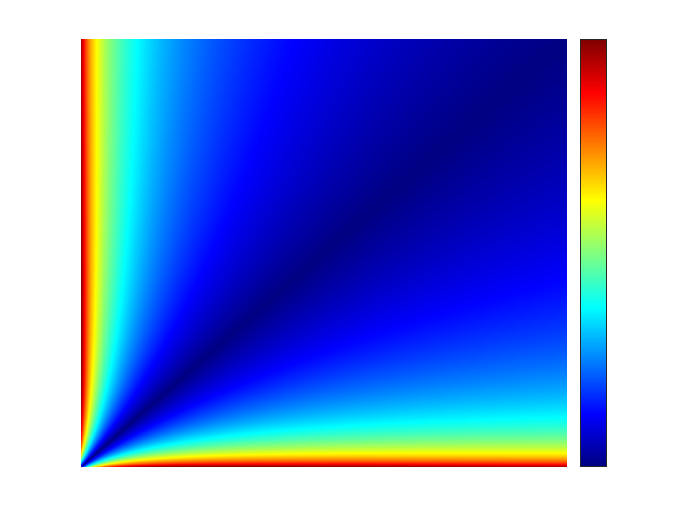
\includegraphics[scale=0.5]{DeltaVHeatmap.png}
    \caption{$\Delta V$ required for a Hohmann transfer between two orbits (created with MATLAB)}\label{fig:Delta V Heatmap}
\end{figure}

In the above figure, $\Delta V$ is represented by the colors, while the axes correspond to the destination and origin orbit radii. It can be seen that the highest $\Delta V$ expenditure occurs when one orbit is very low, while the other is very high.

\bigskip\bigskip
\subsection{Expedited Transfer}

It may at times be the case that the Hohmann Transfer is simply too slow for some applications. If the transfer is from a low orbit to a higher one, then the apoapsis of the transfer orbit can simply be raised higher than the destination orbit.


\begin{figure}[H]
    \centering
    \def\Rone{0.75}
    \def\Rtwo{2.5}
    \def\transSMA{\fpeval{2*\rTwo}}
    \def\ctrX{\fpeval{\Rone-\transSMA}}
    \def\trE{\fpeval{\Rtwo/\transSMA - 1}}
    \def\transSmA{\fpeval{\transSMA*sqrt(1-(\trE)^2)}}
    \def\dV{1.25}
    \definecolor{purp}{rgb}{.8,0,.8}
    \begin{tikzpicture}[>=latex]
        \draw[thin, dotted, blue] (0,0) ellipse ({\Rone} and {\Rone});
        \draw[blue, thick,>-] (-\Rone,0) arc (180:360:{\Rone} and {\Rone}) node[right] {$r_1$};


%        \draw[thin, dotted, purp] (\ctrX,0) ellipse ({\transSMA} and {\transSmA});
%        \draw[purp, thick] (\Rone,0) arc (0:180:{\transSMA} and {\transSmA});

        \draw[thin, dotted,red] (0,0) ellipse ({\Rtwo} and {\Rtwo});
        \draw[red, thick,->] (-\Rtwo,0) arc (180:360:{\Rtwo} and {\Rtwo}) node[right] {$r_2$};;

        \filldraw[lightgray] (0,0) circle (2pt);

        \draw[->] (\Rone,0)--+(0,\dV) node[above] {$\Delta v_1$};
        \draw[->] (-\Rtwo,0)--+(0,-\dV) node[below] {$\Delta v_2$};

    \end{tikzpicture}
    \caption{A Hohmann Transfer from a low orbit to a high orbit (left) and from a high orbit to a lower one (right)}\label{fig:Expedited Transfer}
\end{figure}


%TODO

\bigskip\bigskip
\subsection{Bi-Elliptic Transfer}

A bi-elliptic transfer is another means of transferring from one circular orbit to another. While a Hohmann transfer takes a spacecraft from one circular orbit to another via a singular transfer orbit, the bi-elliptic transfer utilizes a series of two transfer orbits. First, the spacecraft is put into an orbit much higher than either the source or destination orbit. Then, at the apoapsis of the high transfer orbit, the periapsis is brought to the new orbit.

%TODO

\bigskip\bigskip
\subsection{Combined Manuever}

Any single-burn maneuver can be done most efficiently by burning such that $\Delta V$ takes the velocity from some original velocity $\vv{v}_1$ to some desired velocity $\vv{v}_2$. In all probability, the velocity vector of a satellite will be known by measurement. If instead the geometric parameters of the orbit are known, Equations \eqref{Vis-Viva Equation} and \eqref{Flight Path Angle} can be used to determine the velocity vector in the plane of the orbit. The desired velocity vector can be found with the same equations, and using basic trigonometry changes in inclination can be accounted for as well. For maneuvers in which the location of the ascending and descending nodes changes, some geometry must be applied. For any maneuver where the only change in inclination occurs at the ascending or descending node, the calculation is relatively simple. We will assume that the original velocity $v_1$ and the new velocity $v_2$ are both known, the change in flight path angle $\Delta \phi$ is known, and the angle between the old and new orbital planes $\Delta j$ is known. Using this, the total $\Delta V$ required can be calculated. The law of cosines can be used to simplify this calculation, however for ease of following it will not be used.

\begin{align*}
    \Delta V & = |\vv{v}_2-\vv{v}_1|                                                                                                                                           \\
             & = |v_2(\cos(\Delta \phi)\cos(\Delta j)\hat{m}_v+\sin(\Delta \phi)\cos(\Delta j)\hat{m}_r+\sin(\Delta j)\hat{m}_n)-v_1\hat{m}_v|                                 \\
             & = |(v_2\cos(\Delta \phi)\cos(\Delta j)-v_1)\hat{m}_v+v_2\sin(\Delta \phi)\cos(\Delta j)\hat{m}_r+v_2\sin(\Delta j)\hat{m}_n|                                    \\
             & = \sqrt{(v_2\cos(\Delta \phi)\cos(\Delta j)-v_1)^2+(v_2\sin(\Delta \phi)\cos(\Delta j))^2+(v_2\sin(\Delta j))^2}                                                \\
             & = \sqrt{v_2^2\cos^2(\Delta \phi)\cos^2(\Delta j)+v_1^2-2v_1v_2\cos(\Delta \phi)\cos(\Delta j)+v_2^2\sin^2(\Delta \phi)\cos^2(\Delta j)^2+v_2^2\sin^2(\Delta j)} \\
             & = \sqrt{v_1^2+v_2^2\cos^2(\Delta \phi)\cos^2(\Delta j)+v_2^2\sin^2(\Delta \phi)\cos^2(\Delta j)+v_2^2\sin^2(\Delta j)-2v_1v_2\cos(\Delta \phi)\cos(\Delta j)}   \\
             & = \sqrt{v_1^2+v_2^2\cos^2(\Delta j)(\cos^2(\Delta \phi)+\sin^2(\Delta \phi))+v_2^2\sin^2(\Delta j)-2v_1v_2\cos(\Delta \phi)\cos(\Delta j)}                      \\
             & = \sqrt{v_1^2+v_2^2\cos^2(\Delta j)+v_2^2\sin^2(\Delta j)-2v_1v_2\cos(\Delta \phi)\cos(\Delta j)}                                                               \\
             & = \sqrt{v_1^2+v_2^2(\cos^2(\Delta j)+\sin^2(\Delta j))-2v_1v_2\cos(\Delta \phi)\cos(\Delta j)}                                                                  \\
             & = \sqrt{v_1^2+v_2^2-2v_1v_2\cos(\Delta \phi)\cos(\Delta j)}                                                                                                     \\
\end{align*}

For any manuever where the beginning and end velocity vectors are known, the required $\Delta V$ is

\begin{equation}
    \Delta V = \sqrt{v_1^2+v_2^2-2v_1v_2\cos(\Delta \phi)\cos(\Delta j)}
\end{equation}

If instead the angle $\varPhi$ between the vectors is known, this simplifies to

\begin{equation}
    \Delta V = \sqrt{v_1^2+v_2^2-2v_1v_2\cos(\varPhi)}
\end{equation}

\pagebreak
\section{Advanced Maneuvers}

\bigskip\bigskip
\subsection{Gravity Assist}

One maneuver that is used frequently in movies is the gravity assist (sometimes in pop culture referred to as a slingshot maneuver). Intuitively, this may seem to violate what we have learned so far. As a satellite approaches a gravitational source, its velocity increases, trading kinetic energy for potential energy. However, as the satellite departs from the gravitational source, the tradeoff will occur in reverse, with no kinetic energy being gained. This would seem to imply that a spacecraft cannot gain speed just by flinging around a planet.

A flyby will take the shape of a hyperbolic trajectory, entering at some angle relative to reference direction and leaving at some other angle. From Equation \eqref{Vis-Viva Equation}, the speed is only distance-dependant. A spacecraft's velocity at some distance $r$ from the gravity source will not change whether the spacecraft is approaching the gravity source or leaving it. Of course, the existence of a gravity assist maneuver means that there must be some error in this logic.

For the sake of this exploration, a gravity assist from Jupiter in a solar orbit will be considered.

\begin{figure}[H]
    \centering
    \begin{tikzpicture}[>=latex]
        \def\ecc{1.2}
        \def\arcRad{1}
        \def\m{\fpeval{sqrt(\ecc^2-1)}}
        \def\endT{2}

        \coordinate (p1) at (-{cosh(\endT)+\ecc},{-\m*sinh(\endT)}) {};
        \coordinate (p2) at (-{cosh(\endT)+\ecc},{\m*sinh(\endT)}) {};

        \draw[scale=1,domain=-\endT:\endT,smooth,variable=\t, thin, densely dotted] plot ({-cosh(\t)+\ecc},{-\m*sinh(\t)});
        \filldraw[brown] (0,0) circle (2pt);

        \filldraw[gray] (p1) circle (1pt);
        \filldraw[gray] (\ecc-1,0) circle (1pt);
        \filldraw[gray] (p2) circle (1pt);

        \draw[gray, ->] (p1) node[below right] {$v_1$} -- +(0.5,0.5*\m);
        \draw[gray, ->] (\ecc-1,0) -- +(0,1) node[right] {$v_2>v_1$};
        \draw[gray, ->] (p2) node[above right] {$v_3=v_1$} -- +(-0.5,0.5*\m);
    \end{tikzpicture}
    \caption{A hyperbolic trajectory of a satellite (gray) past Jupiter (brown)}\label{fig:Jupiter Flyby}
\end{figure}

The critical piece that is missing from this understanding so far is the relative nature of velocity. Equations so far have all been in terms of the body being orbited. It is indeed true that, in the above image, $|v_3|=|v_1|$ relative to Jupiter. However, this is not the complete picture. When in a hyperbolic trajectory past Jupiter, the spacecraft's speed \textit{relative to Jupiter} is dependant only on its position. However, relative to the sun this may not be true.

Figure \ref{fig:Jupiter Flyby} can be redrawn to include velocities relative to the sun. It will be decided that Jupiter is moving to the left sun. The sun will not be shown. Velocities relative to the sun will be drawn in red, while velocities relative to Jupiter will be drawn in brown. Subscripts $j$ and $s$ mean relative to Jupiter and to the sun, respectively.

\begin{figure}[H]
    \centering
    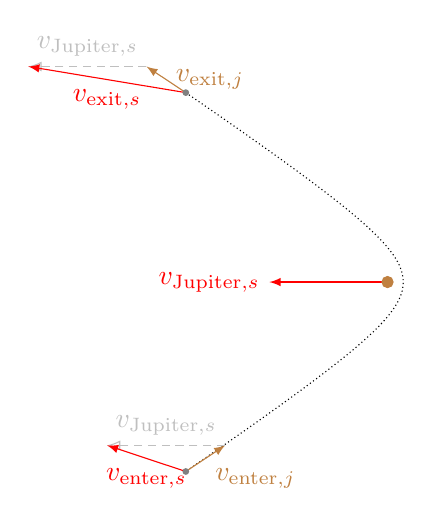
\begin{tikzpicture}[>=latex]
        \def\ecc{1.2}
        \def\arcRad{1}
        \def\m{\fpeval{sqrt(\ecc^2-1)}}
        \def\endT{2}
        \def\vJ{1.5}

        \coordinate (p1) at (-{cosh(\endT)+\ecc},{-\m*sinh(\endT)}) {};
        \coordinate (p2) at (-{cosh(\endT)+\ecc},{\m*sinh(\endT)}) {};
        \coordinate (vJup) at (-\vJ,0) {};

        \draw[scale=1,domain=-\endT:\endT,smooth,variable=\t, thin, densely dotted] plot ({-cosh(\t)+\ecc},{-\m*sinh(\t)});


        \draw[red, ->] (0,0) -- (vJup) node[left] {$v_{\text{Jupiter},s}$};
        \draw[brown, ->] (p1) -- +(0.5,0.5*\m) node[midway, below right] {$v_{\text{enter},j}$};
        \draw[brown, ->] (p2) -- +(-0.5,0.5*\m) node[midway, right] {$v_{\text{exit},j}$};

        \draw[lightgray, thin, densely dashed, -{Latex[open]}] (p1)++(0.5,0.5*\m)--+(vJup) node[midway, above] {$v_{\text{Jupiter},s}$};
        \draw[lightgray, thin, densely dashed, -{Latex[open]}] (p2)++(-0.5,0.5*\m)--+(vJup) node[midway, above] {$v_{\text{Jupiter},s}$};

        \draw[red, ->] (p1) -- + (0.5-\vJ,0.5*\m) node[midway, below] {$v_{\text{enter},s}$};
        \draw[red, ->] (p2) --+ (-0.5-\vJ,0.5*\m) node[midway, below] {$v_{\text{exit},s}$};


        \filldraw[gray] (p1) circle (1pt);
        \filldraw[gray] (p2) circle (1pt);
        \filldraw[brown] (0,0) circle (2pt);
    \end{tikzpicture}
    \caption{Jupiter Flyby With Relative Velocities}\label{fig:Jupiter Flyby Rel Velocities}
\end{figure}

Note that Jupiter's velocity relative to the sun is also shown at the spacecraft's location in order to make the vector addition visually intuitive. As can be seen in Figure \ref{fig:Jupiter Flyby Rel Velocities}, the spacecraft's velocity relative to the sun is changed by Jupiter.

While this may seem to violate conservation of energy and momentum, it does not. Any momentum or energy gained by the spacecraft will be lost by the planet that's providing the gravity assist. While this does have an effect on the orbit of the planet that's providing a gravity assist (Jupiter, in this case), this effect is negligible. Jupiter has a mass on the order of 10\textsuperscript{27} kilograms, while most satellites will have masses between 10\textsuperscript{2} and 10\textsuperscript{4} kilograms. This means that an energy transfer that tremendously impacts the velocity of a satellite will have a negligible effect on Jupiter.

To illustrate the varying effects that gravity assists can have, a few possible assists will be drawn.

\begin{figure}[H]
    \centering
    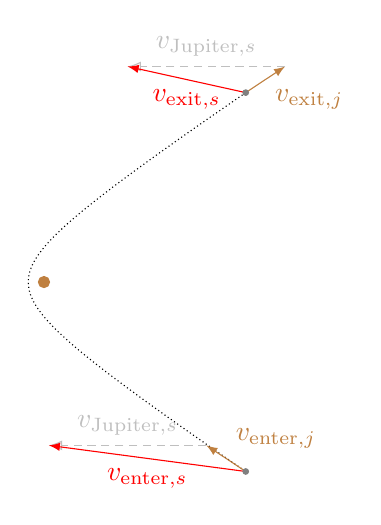
\begin{tikzpicture}[>=latex]
        \def\ecc{1.2}
        \def\arcRad{1}
        \def\m{\fpeval{sqrt(\ecc^2-1)}}
        \def\endT{2}
        \def\vJ{2}

        \coordinate (p1) at ({cosh(\endT)-\ecc},{-\m*sinh(\endT)}) {};
        \coordinate (p2) at ({cosh(\endT)-\ecc},{\m*sinh(\endT)}) {};
        \coordinate (vJup) at (-\vJ,0) {};

        \draw[scale=1,domain=-\endT:\endT,smooth,variable=\t, thin, densely dotted] plot ({cosh(\t)-\ecc},{-\m*sinh(\t)});


        \draw[brown, ->] (p1) -- +(-0.5,0.5*\m) node[midway, above right] {$v_{\text{enter},j}$};
        \draw[brown, ->] (p2) -- +(0.5,0.5*\m) node[midway, below right] {$v_{\text{exit},j}$};

        \draw[lightgray, thin, densely dashed, -{Latex[open]}] (p1)++(-0.5,0.5*\m)--+(vJup) node[midway, above] {$v_{\text{Jupiter},s}$};
        \draw[lightgray, thin, densely dashed, -{Latex[open]}] (p2)++(0.5,0.5*\m)--+(vJup) node[midway, above] {$v_{\text{Jupiter},s}$};

        \draw[red, ->] (p1) -- + (-0.5-\vJ,0.5*\m) node[midway, below] {$v_{\text{enter},s}$};
        \draw[red, ->] (p2) --+ (0.5-\vJ,0.5*\m) node[midway, below] {$v_{\text{exit},s}$};


        \filldraw[gray] (p1) circle (1pt);
        \filldraw[gray] (p2) circle (1pt);
        \filldraw[brown] (0,0) circle (2pt);
    \end{tikzpicture}
    \caption{Gravity Assist In Front of Planet}\label{fig:Gravity Assist Ahead of Planet}
\end{figure}

From Figures \ref{fig:Jupiter Flyby Rel Velocities} and \ref{fig:Gravity Assist Ahead of Planet}, it is clear that passing behind the planet acts to accelerate the spacecraft, while passing behind the planet decelerates the spacecraft by the same amount. Note that, while these orbits both start "below" Jupiter and end "above" it, the effect is the exact same if the direction of the flyby is reversed. Visualization of this effect is left as an exercise to the reader. Next, the effect of passing "above" or "below" the planet will be investigated.

\begin{figure}[H]
    \centering
    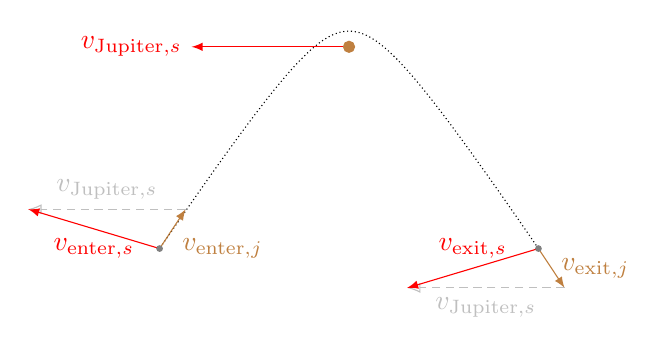
\begin{tikzpicture}[>=latex]
        \def\ecc{1.2}
        \def\arcRad{1}
        \def\m{\fpeval{sqrt(\ecc^2-1)}}
        \def\endT{2}
        \def\vJ{2}

        \coordinate (p1) at ({-\m*sinh(\endT)},-{cosh(\endT)+\ecc}) {};
        \coordinate (p2) at ({\m*sinh(\endT)}, -{cosh(\endT)+\ecc}) {};
        \coordinate (vJup) at (-\vJ,0) {};

        \draw[scale=1,domain=-\endT:\endT,smooth,variable=\t, thin, densely dotted] plot ({-\m*sinh(\t)},{-cosh(\t)+\ecc});

        \draw[red, ->] (0,0) -- (vJup) node[left] {$v_{\text{Jupiter},s}$};
        \draw[brown, ->] (p1) -- +(0.5*\m, 0.5) node[midway, below right] {$v_{\text{enter},j}$};
        \draw[brown, ->] (p2) -- +(0.5*\m, -0.5) node[midway, right] {$v_{\text{exit},j}$};

        \draw[lightgray, thin, densely dashed, -{Latex[open]}] (p1)++(0.5*\m, 0.5)--+(vJup) node[midway, above] {$v_{\text{Jupiter},s}$};
        \draw[lightgray, thin, densely dashed, -{Latex[open]}] (p2)++(0.5*\m, -0.5)--+(vJup) node[midway, below] {$v_{\text{Jupiter},s}$};

        \draw[red, ->] (p1) -- + (0.5*\m-\vJ,0.5) node[midway, below] {$v_{\text{enter},s}$};
        \draw[red, ->] (p2) --+ (0.5*\m-\vJ,-0.5) node[midway, above] {$v_{\text{exit},s}$};

        \filldraw[gray] (p1) circle (1pt);
        \filldraw[gray] (p2) circle (1pt);
        \filldraw[brown] (0,0) circle (2pt);

    \end{tikzpicture}
    \caption{Radial Gravity Assists}\label{fig:Gravity assists above/below}
\end{figure}

In Figure \ref{fig:Gravity assists above/below}, the magnitude of velocity of the satellite did not change; instead, its direction changed. The planet has the net effect of redirecting the spacecraft's velocity with respect to the planet that is giving the gravity assist.

In Figures \ref{fig:Jupiter Flyby}, \ref{fig:Jupiter Flyby Rel Velocities}, \ref{fig:Gravity Assist Ahead of Planet}, and \ref{fig:Gravity assists above/below}, the hyperbolic flyby had the same eccentricity (precisely 1.2). However, the direction and eccentricity of the flyby can be fine-tuned to ensure the desired effect on the spacecraft's orbit.

\subsubsection{Mathematical Analysis of Gravity Assists}

Because a hyperbolic trajectory occurs above escape velocity (See Equation \eqref{Orbit Shape Physical}), the speed that the spacecraft approaches (relative to the planet) in the limit can be determined.

\begin{align*}
    v_\infty & = \lim_{r\rightarrow\infty}v                                                \\
             & = \lim_{r\rightarrow\infty}\left(\sqrt{\frac{2\mu}{r}-\frac{\mu}{a}}\right) \\
             & = \sqrt{\frac{\mu}{-a}}
\end{align*}

Using this, the semi-major axis can be found
\begin{align*}
    v_\infty   & = \sqrt{\frac{\mu}{-a}}   \\
    v_\infty^2 & = \frac{\mu}{-a}          \\
    a          & = \frac{-\mu}{v_\infty^2} \\
\end{align*}

The semi-major axis is uniquely determined by the limiting velocity of the spacecraft, and is unaffected by the entry/exit angle $\theta_\text{hyp}$. A more useful way of phrasing this is that the entry/exit angle is unaffected by the entry velocity.

Because $a$ is not determined by the chosen hyperbolic trajectory, from Equation \eqref{Periapsis Radius Geometric} the eccentricity can be determined by the periapsis radius. Solving Equation \eqref{Periapsis Radius Geometric} for the eccentricity,

\begin{align*}
    r_\text{pe}                       & =a(1-e)                       \\
    r_\text{pe}                       & =\frac{-\mu}{v_\infty^2}(1-e) \\
    r_\text{pe}                       & =\frac{\mu}{v_\infty^2}(e-1)  \\
    \frac{r_\text{pe}v_\infty^2}{\mu} & =e-1                          \\
\end{align*}
\begin{equation}\label{Hyperbolic Flyby Eccentricity}
    e=\frac{r_\text{pe}v_\infty^2}{\mu}+1
\end{equation}

Recall from Equation \eqref{Hyperbolic entry/exit angle} that $\theta_\text{hyp}$ is determined uniquely by $e$.

\begin{align*}
    \theta_\text{hyp} & =\arctan\left(\sqrt{e^2-1}\right)                                                \\
                      & =\arctan\left(\sqrt{\left(\frac{r_\text{pe}v_\infty^2}{\mu}+1\right)^2-1}\right) \\
\end{align*}

\begin{equation}\label{Hyperbola angle in terms of pe}
    \theta_\text{hyp}=\arctan\left(\sqrt{\left(\frac{r_\text{pe}v_\infty^2}{\mu}+1\right)^2-1}\right)\\
\end{equation}

With Equation \eqref{Hyperbola angle in terms of pe}, we now have the tools to determine the effect of a gravity assist on a spacecraft's velocity relative to the sun. For the sake of simplicity, the argument of $\arctan$ in Equation \eqref{Hyperbola angle in terms of pe} will be referred to as simply $m_\text{hyp}$

The net change in a spacecraft's velocity vector relative to the sun can be expressed as follows. Subscripts $s$ and $p$ will be used to denote velocity relative to a planet versus that relative to the sun. The maneuvering basis vectors are relative to $\vv{v}_{\text{enter},p}$. The exit velocity vector will be rotated by $2\theta_\text{hyp}$, and then reversed in direction (See figure \ref{fig:Hyperbolic Trajectory}). This has the net effect of a rotation of $\pi-2\theta_\text{hyp}$ Recall also that $\hat{m}_r$ points \textit{out} of the orbit.

\begin{align*}
    \Delta\vv{v}_s & = \Delta\vv{v}_p                                                                                             \\
                   & = \vv{v}_{\text{exit},p}-\vv{v}_{\text{enter},p}                                                             \\
                   & = v_\infty\hat{v}_{\text{exit},p}-v_\infty\hat{v}_{\text{enter},p}                                           \\
                   & = v_\infty(\cos(\pi-2\theta_\text{hyp})\hat{m}_v-\sin(\pi-2\theta_\text{hyp})(-\hat{m}_r))-v_\infty\hat{m}_v \\
                   & = v_\infty(\cos(\pi-2\theta_\text{hyp})\hat{m}_v+\sin(\pi-2\theta_\text{hyp})\hat{m}_r)-v_\infty\hat{m}_v    \\
                   & = v_\infty(-\cos(2\theta_\text{hyp})\hat{m}_v+\sin(2\theta_\text{hyp})\hat{m}_r)-v_\infty\hat{m}_v           \\
                   & = v_\infty((-1-\cos(2\theta_\text{hyp}))\hat{m}_v+\sin(2\theta_\text{hyp})\hat{m}_r)                         \\
                   & = v_\infty(-(1+\cos(2\theta_\text{hyp}))\hat{m}_v+\sin(2\theta_\text{hyp})\hat{m}_r)                         \\
                   & = v_\infty(-(1+\cos(2\arctan(m_\text{hyp})))\hat{m}_v+\sin(2\arctan(m_\text{hyp}))\hat{m}_r)                 \\
\end{align*}

It can be shown from trigonometry that
$$\cos(2\arctan(\theta))=\frac{1-\theta^2}{1+\theta^2}\qquad\text{and}\qquad\sin(2\arctan(\theta))=\frac{2\theta}{1+\theta^2}$$

%\left(\sqrt{\left(\frac{r_\text{pe}v_\infty^2}{\mu}+1\right)^2-1}\right)

\begin{align*}
    \Delta\vv{v}_s & = v_\infty(-(1+\cos(2\arctan(m_\text{hyp})))\hat{m}_v+\sin(2\arctan(m_\text{hyp}))\hat{m}_r)                                                                                                                                                                                                               \\
                   & = v_\infty\left(-\left(1+\frac{1-m_\text{hyp}^2}{1+m_\text{hyp}^2}\right)\hat{m}_v+\frac{2m_\text{hyp}}{1+m_\text{hyp}^2}\hat{m}_r\right)                                                                                                                                                                  \\
                   & = v_\infty\left(-\left(1+\frac{1-\left(\frac{r_\text{pe}v_\infty^2}{\mu}+1\right)^2+1}{1+\left(\frac{r_\text{pe}v_\infty^2}{\mu}+1\right)^2-1}\right)\hat{m}_v+\frac{2\sqrt{\left(\frac{r_\text{pe}v_\infty^2}{\mu}+1\right)^2-1}}{1+\left(\frac{r_\text{pe}v_\infty^2}{\mu}+1\right)^2-1}\hat{m}_r\right) \\
                   & = v_\infty\left(-\left(\frac{2}{\left(\frac{r_\text{pe}v_\infty^2}{\mu}+1\right)^2}\right)\hat{m}_v+\frac{2\sqrt{\left(\frac{r_\text{pe}v_\infty^2}{\mu}+1\right)^2-1}}{\left(\frac{r_\text{pe}v_\infty^2}{\mu}+1\right)^2}\hat{m}_r\right)                                                                \\
                   & = v_\infty\left(\frac{-2}{\left(\frac{r_\text{pe}v_\infty^2}{\mu}+1\right)^2}\hat{m}_v+\frac{2\sqrt{\left(\frac{r_\text{pe}v_\infty^2}{\mu}+1\right)^2-1}}{\left(\frac{r_\text{pe}v_\infty^2}{\mu}+1\right)^2}\hat{m}_r\right)                                                                             \\
\end{align*}

While this may not intuitively seem that useful (and, frankly, it isn't), the magnitude proves to be much simpler.

\begin{align*}
    |\Delta\vv{v}_s| & = v_\infty\left|\frac{-2}{\left(\frac{r_\text{pe}v_\infty^2}{\mu}+1\right)^2}\hat{m}_v+\frac{2\sqrt{\left(\frac{r_\text{pe}v_\infty^2}{\mu}+1\right)^2-1}}{\left(\frac{r_\text{pe}v_\infty^2}{\mu}+1\right)^2}\hat{m}_r\right|       \\
                     & = v_\infty\sqrt{\left(\frac{-2}{\left(\frac{r_\text{pe}v_\infty^2}{\mu}+1\right)^2}\right)^2+\left(\frac{2\sqrt{\left(\frac{r_\text{pe}v_\infty^2}{\mu}+1\right)^2-1}}{\left(\frac{r_\text{pe}v_\infty^2}{\mu}+1\right)^2}\right)^2} \\
                     & = v_\infty\sqrt{\frac{4}{\left(\frac{r_\text{pe}v_\infty^2}{\mu}+1\right)^4}+\frac{4\left(\left(\frac{r_\text{pe}v_\infty^2}{\mu}+1\right)^2-1\right)}{\left(\frac{r_\text{pe}v_\infty^2}{\mu}+1\right)^4}}                          \\
                     & = 2v_\infty\sqrt{\frac{1+\left(\frac{r_\text{pe}v_\infty^2}{\mu}+1\right)^2-1}{\left(\frac{r_\text{pe}v_\infty^2}{\mu}+1\right)^4}}                                                                                                  \\
                     & = 2v_\infty\sqrt{\frac{\left(\frac{r_\text{pe}v_\infty^2}{\mu}+1\right)^2}{\left(\frac{r_\text{pe}v_\infty^2}{\mu}+1\right)^4}}                                                                                                      \\
                     & = 2v_\infty\sqrt{\frac{1}{\left(\frac{r_\text{pe}v_\infty^2}{\mu}+1\right)^2}}                                                                                                                                                       \\
                     & = \frac{2v_\infty}{\frac{r_\text{pe}v_\infty^2}{\mu}+1}                                                                                                                                                                              \\
\end{align*}

The magnitude of $\Delta V$ from a gravity assist is
\begin{equation}\label{Gravity Assist Delta V}
    \Delta V_\text{assist}=\frac{2\mu_p v_\infty}{r_\text{pe}v_\infty^2+\mu_p}\\
\end{equation}

Where $\mu_p$ refers to the standard gravitational parameter of the planet that is giving a gravity assist.

The direction of this gravity assist is the direction of the change relative velocity of the planet. From Figures \ref{fig:Jupiter Flyby Rel Velocities}, \ref{fig:Gravity Assist Ahead of Planet}, and \ref{fig:Gravity assists above/below}, the direction of change in velocity is the vector facing from the periapsis of the hyperbola to the planet.

Equation \eqref{Gravity Assist Delta V} can be optimized to find the peak $\Delta V$. It is clear that any decrease in $r_\text{pe}$ will increase the $\Delta V$, so the optimization will be for peak $v_\infty$. This will be done by differentiating \eqref{Gravity Assist Delta V} with respect to $v_\infty$, and setting the derivative to zero.

\begin{align*}
    \frac{d}{dv_\infty}\Delta V_\text{assist} & =\frac{d}{dv_\infty}\Delta\left(\frac{2\mu_p v_\infty}{r_\text{pe}v_\infty^2+\mu_p}\right)                                                         \\
                                              & =\frac{d}{dv_\infty}\left(\frac{2\mu_p v_\infty}{r_\text{pe}v_\infty^2+\mu_p}\right)                                                               \\
                                              & =2\mu_p\frac{d}{dv_\infty}\left(v_\infty(r_\text{pe}v_\infty^2+\mu_p)^{-1}\right)                                                                  \\
                                              & =2\mu_p\left(v_\infty\frac{d}{dv_\infty}(r_\text{pe}v_\infty^2+\mu_p)^{-1}+(r_\text{pe}v_\infty^2+\mu_p)^{-1}\frac{d}{dv_\infty}v_\infty\right)    \\
                                              & =2\mu_p\left(-v_\infty(r_\text{pe}v_\infty^2+\mu_p)^{-2}\frac{d}{dv_\infty}(r_\text{pe}v_\infty^2+\mu_p)+(r_\text{pe}v_\infty^2+\mu_p)^{-1}\right) \\
                                              & =2\mu_p\left(-v_\infty(r_\text{pe}v_\infty^2+\mu_p)^{-2}(2r_\text{pe}v_\infty)+(r_\text{pe}v_\infty^2+\mu_p)^{-1}\right)                           \\
                                              & =2\mu_p\left(\frac{-2r_\text{pe}v_\infty^2}{(r_\text{pe}v_\infty^2+\mu_p)^2}+\frac{1}{r_\text{pe}v_\infty^2+\mu_p}\right)                          \\
                                              & =2\mu_p\left(\frac{-2r_\text{pe}v_\infty^2+r_\text{pe}v_\infty^2+\mu_p}{(r_\text{pe}v_\infty^2+\mu_p)^2}\right)                                    \\
                                              & =2\mu_p\left(\frac{-r_\text{pe}v_\infty^2+\mu_p}{(r_\text{pe}v_\infty^2+\mu_p)^2}\right)                                                           \\
\end{align*}

Now, this will be set to zero to find $v_\infty$ for maximum $\Delta V$
\begin{align*}
    2\mu_p\left(\frac{-r_\text{pe}v_\infty^2+\mu_p}{(r_\text{pe}v_\infty^2+\mu_p)^2}\right) & = 0                                \\
    \frac{-r_\text{pe}v_\infty^2+\mu_p}{(r_\text{pe}v_\infty^2+\mu_p)^2}                    & = 0                                \\
    -r_\text{pe}v_\infty^2+\mu_p                                                            & = 0                                \\
    r_\text{pe}v_\infty^2                                                                   & = \mu_p                            \\
    v_\infty^2                                                                              & = \frac{\mu_p}{r_\text{pe}}        \\
    v_\infty                                                                                & = \sqrt{\frac{\mu_p}{r_\text{pe}}} \\
\end{align*}

Notice that this is equal to the velocity for a circular orbit at periapsis.
\begin{equation}\label{Gravity Assist Best Vinfty}
    v_{\infty,\text{best}} = \sqrt{\frac{\mu_p}{r_\text{pe}}} = v_\text{circ@pe}
\end{equation}

This can be plugged into Equation \eqref{Gravity Assist Delta V} to find the optimal $\Delta V$ for a gravity assist.
\begin{align*}
    \Delta V_\text{assist} & =\frac{2\mu_p v_\infty}{r_\text{pe}v_\infty^2+\mu_p}                                                              \\
                           & =\frac{2\mu_p \sqrt{\frac{\mu_p}{r_\text{pe}}}}{r_\text{pe}\left(\sqrt{\frac{\mu_p}{r_\text{pe}}}\right)^2+\mu_p} \\
                           & =\frac{2\mu_p \sqrt{\frac{\mu_p}{r_\text{pe}}}}{2\mu_p}                                                           \\
                           & =\sqrt{\frac{\mu_p}{r_\text{pe}}}
\end{align*}

The maximum $\Delta V$ from a gravity assist occurs when the limiting velocity of the satellite is $v_\infty=\sqrt{\frac{\mu_p}{r_\text{pe}}}$, and it results in an assist with $\Delta V = \sqrt{\frac{\mu_p}{r_\text{pe}}}$ along the vector pointing from periapsis to the planet.

For the sake of curiosity, we shall now find (using Equation \eqref{Hyperbolic Flyby Eccentricity}) the eccentricity that this hyperbolic trajectory will have.

\begin{align*}
    e & = \frac{r_\text{pe}v_\infty^2}{\mu_p}+1                   \\
      & = \frac{r_\text{pe}(\sqrt{\mu_p/r_\text{pe}})^2}{\mu_p}+1 \\
      & = \frac{r_\text{pe}(\mu_p/r_\text{pe})}{\mu_p}+1          \\
      & = \frac{r_\text{pe}\mu_p}{\mu_p r_\text{pe}}+1            \\
      & = 1+1                                                     \\
      & = 2
\end{align*}

The eccentricity to maximize $\Delta V$ of a gravity assist is $e=2$. Equation \eqref{Hyperbolic entry/exit angle} shows that this gives $\theta_\text{hyp}=60^{\circ}=\frac{\pi}{3}$.

\subsubsection{Gravity Assist Conclusion}

The term "gravity assist" is possibly a bit of a misnomer, as the gravity serves only to redirect the velocity of the spacecraft, but does not change its magnitude. A spacecraft can be accelerated in its orbit by a planet if it passes behind the planet. Really what's happening is the spacecraft is using the planet's mass to redirect its speed, resulting in a change in the spacecraft's orbit. A well-timed flyby can act to change the velocity of the spacecraft in many different directions. From equation \eqref{Gravity Assist Delta V}, it can be seen that $\Delta V$ is maximized by minimizing $r_\text{pe}$ and bringing $v_\infty$ as close as possible to $\sqrt{\frac{\mu_p}{r_\text{pe}}}$. At this value for $v_\infty$, $\Delta V = \sqrt{\frac{\mu_p}{r_\text{pe}}}$ and the hyperbola will have an eccentricity of $e=2$. It can also be seen that the greater the mass of the planet (and therefore $\mu$), the larger the effect will be. Another way of stating this is that to maximize the effect of a gravity assist, the hyperbolic trajectory should maximize its change in direction, which means minimizing its eccentricity (provided the eccentricity is greater than one). From Equation \eqref{Hyperbolic Flyby Eccentricity}, it can be seen that this entails minimizing $r_\text{pe}$ for any given $v_\infty$.

%TODO: Patched Conics
%TODO: Lagrange Points

\pagebreak
\section{Appendix}
\bigskip\bigskip
\subsection{Orbit Planar Geometry}

\begin{figure}[H]
    \centering
    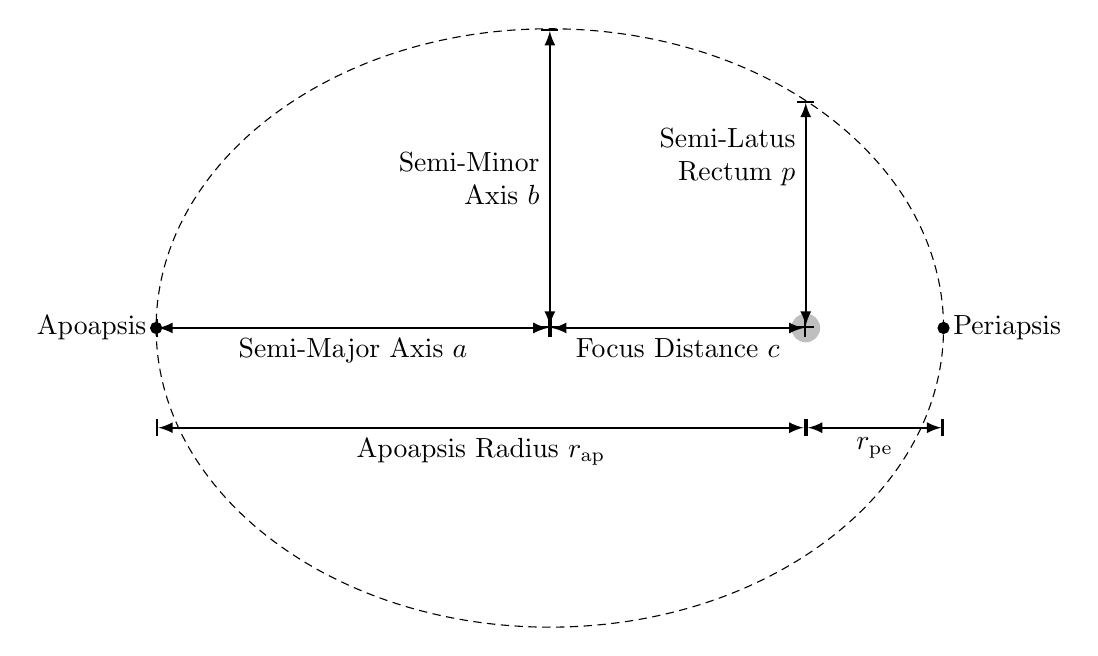
\begin{tikzpicture}[>=latex]
        \def\ecc{0.65}
        \def\SMA{5}
        \def\ap{\fpeval{\SMA*(1+\ecc)}}
        \def\pe{\fpeval{\SMA*(1-\ecc)}}
        \def\slr{\fpeval{\SMA*(1-(\ecc)^2)}}
        \def\SmA{\fpeval{\SMA*(1-(\ecc)^2)^(1/2)}}

        \draw[thin, densely dashed] (0,0) ellipse ({\SMA} and {\SmA});
        \filldraw[lightgray] (\ap-\SMA,0) circle (5pt);

        \draw[|<->|, thick] (-\SMA, 0) -- (0, 0) node[midway, below] {Semi-Major Axis $a$};
        \draw[|<->|, thick] (0, 0) -- (0, \SmA) node[align=right, midway, left] {Semi-Minor\\Axis $b$};
        \draw[|<->|, thick] (\ap-\SMA, 0) -- (\ap-\SMA, \slr) node[align=right, near end, left] {Semi-Latus\\Rectum $p$};

        \draw[|<->|, thick] (0,0) -- (\ap-\SMA,0) node[midway, below] {Focus Distance $c$};

        \draw[|<->|, thick] (\ap-\SMA, -\SmA/3) -- (\SMA, -\SmA/3) node[midway, below] {$r_\text{pe}$};

        \draw[|<->|, thick] (-\SMA, -\SmA/3) -- (\ap-\SMA, -\SmA/3) node[midway, below] {Apoapsis Radius $r_\text{ap}$};

        \filldraw[] (\SMA,0) circle (2pt) node[right] {Periapsis};
        \filldraw[] (-\SMA,0) circle (2pt) node[left] {Apoapsis};

    \end{tikzpicture}

    \caption{An orbit with important geometric values labeled}\label{fig:Orbit Diagram}
\end{figure}

In the above figure, the semi-major axis $a$, semi-minor axis $b$, semi-latus rectum $p$, focus distance $c$, apoapsis radius $r_\text{ap}$, and periapsis radius $r_\text{pe}$ are all labeled. The apoapsis is the highest point in the orbit, and the periapsis is the lowest. The major axis is the largest distance across the ellipse, while the minor axis is the smallest. The latus rectum is the width of the ellipse perpendicular to the foci. The focus distance is the distance between the foci and the center of the ellipse.


\bigskip\bigskip
\subsection{Positional Diagram}
\begin{figure}[H]
    \centering
    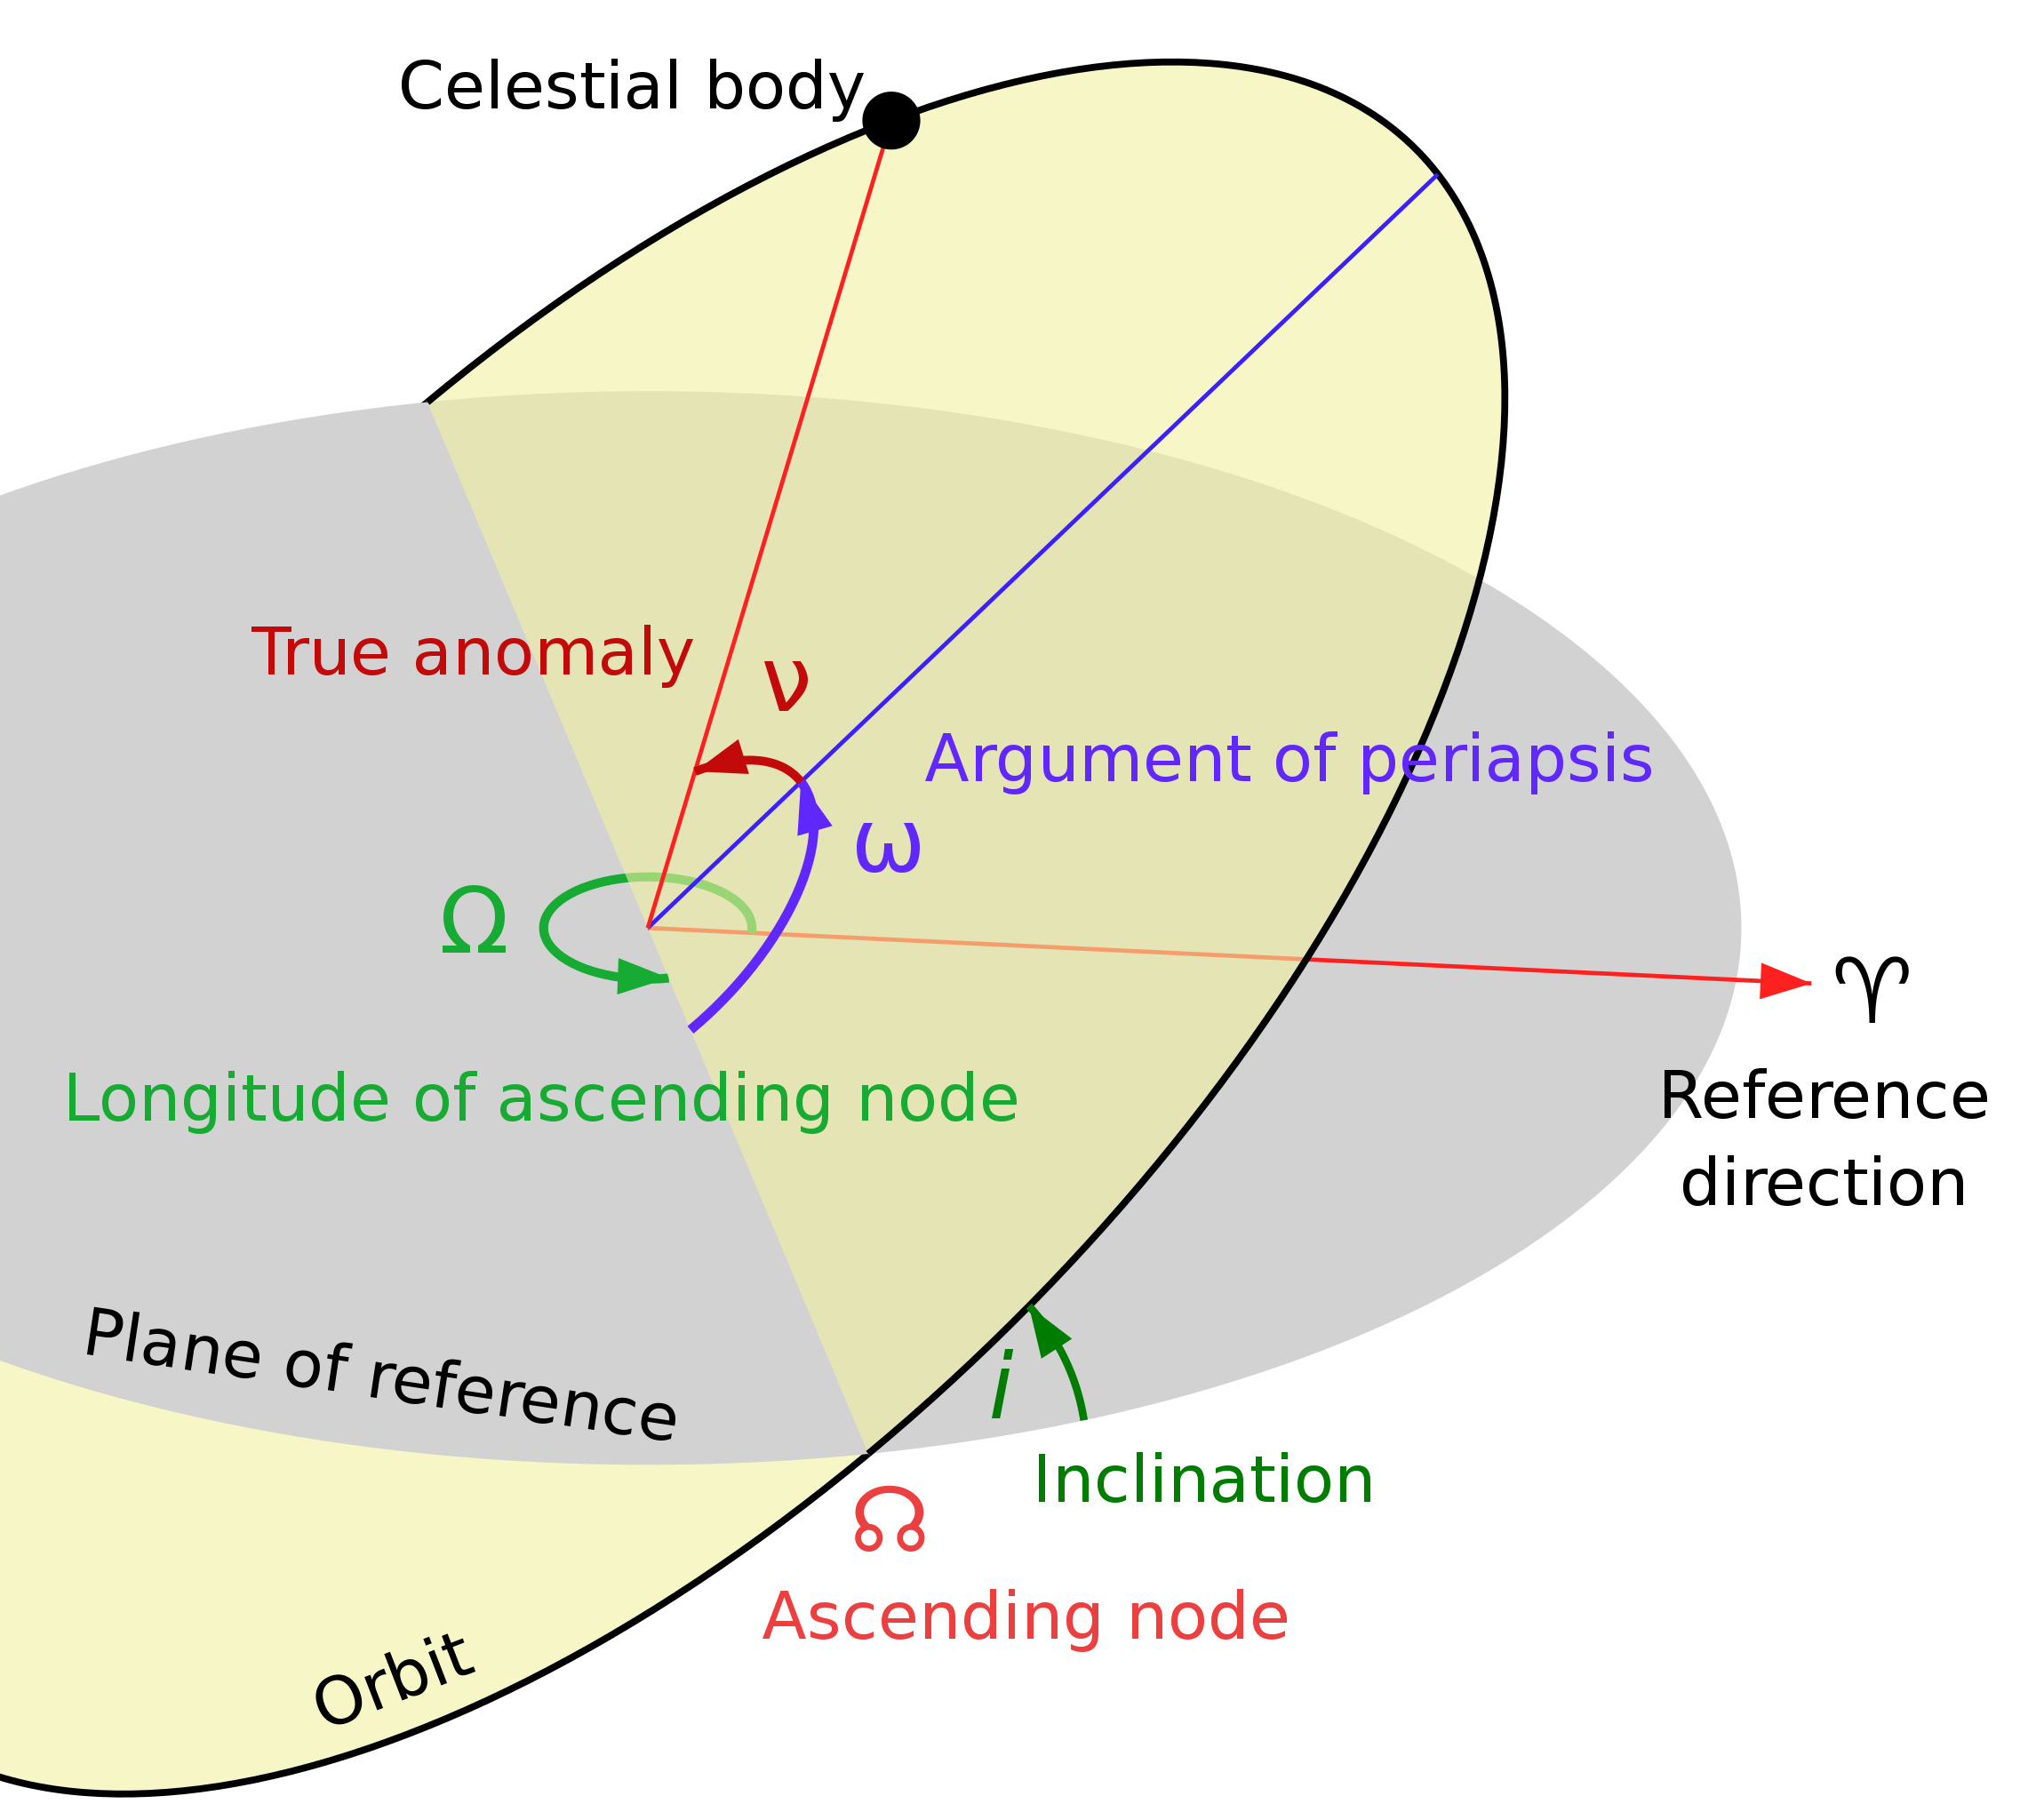
\includegraphics[scale=0.1]{WikiImage}
    \caption{Figure from wikipedia.org showing orbital elements}\label{fig:Wiki Image}
\end{figure}
There are a variety of parameters that are used to position the orbit in space, and to position the satellite in the orbit. Note that $\nu$ (nu) and $\theta$ (theta) are used interchangeably, with $\theta$ being used predominantly in this document. The blue line points to the periapsis. Note also that the blue line and the red line are not necessarily aligned with eachother.

The base frame $a$ can be defined such that $\hat{a}_1$ points in the reference direction, $\hat{a}_2$ points 90 degrees clockwise of the reference direction in place with the reference plane, and $\hat{a}_3$ pointing normal to the base frame (generally "up" in the image above).

Another frame $b$ can be defined such that $b$ is the same as the $a$ frame, but rotated $\Omega$ about $\hat{a}_3$. This means that $\hat{b}_1$ points toward the ascending node, $\hat{b}_2$ is normal to $\hat{b}_1$ and in the reference plane, and $\hat{b}_3=\hat{a}_3$.

Frame $c$ can be defined as a rotation of frame $b$ about $\hat{b}_1$ by $i$. This frame is in the plane of the orbit, with $\hat{c}_1=\hat{b}_1$ and $\hat{c}_3$ being normal to the orbit.

Next, $d$ can be defined as a rotation of $c$ by $\omega$ about $\hat{c}_3$. This frame is also in the plane of the orbit, with $\hat{c}_1$ pointing toward the periapsis.

Finally, another frame can be defined as a rotation of $d$ by $\theta$ about $\hat{d}_3$. This creates the polar frame (see Figures \ref{fig:Coordinate System} and \ref{fig:Coordinate System 3D}).

\begin{figure}[H]
    \centering
    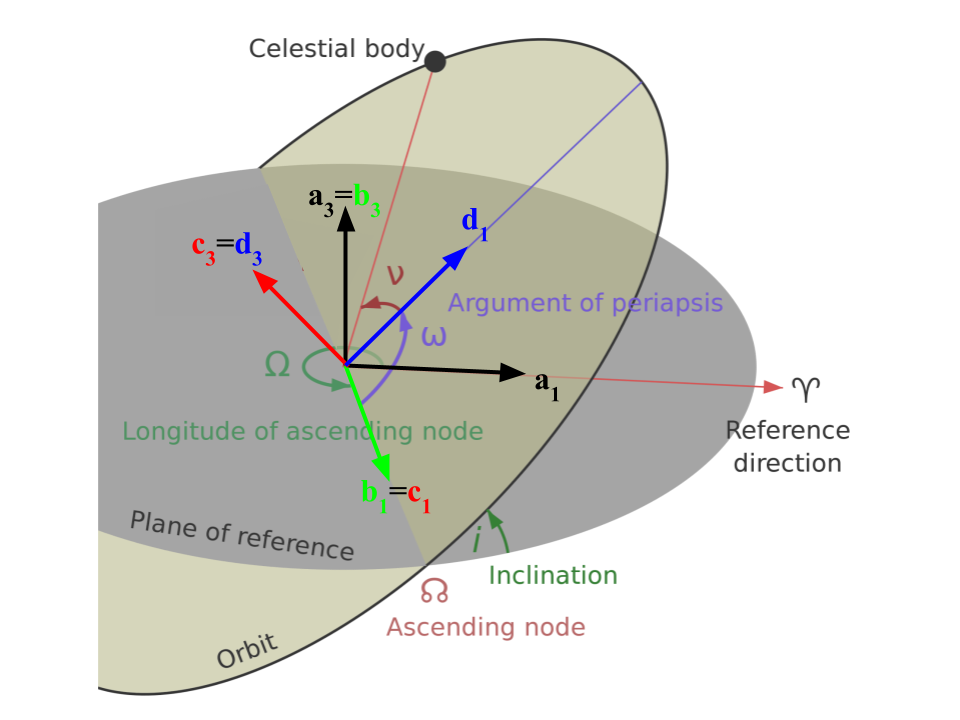
\includegraphics[scale=0.3]{Frames}
    \caption{Reference frames (aside from polar and maneuvering frames)}\label{fig:Frames}
\end{figure}

To get a better sense for how orbital parameters work, it is highly reccomended that the reader experiment with https://orbitalmechanics.info/

\bigskip\bigskip
\subsection{Orbit elements}

\begin{comment}
\begin{figure}[H]
    \centering
    \def\SMA{3}
    \def\inc{20}

    \tdplotsetmaincoords{70}{40}
    \begin{tikzpicture}[tdplot_main_coords, >=latex]
        \tdplotsetrotatedcoords{0}{-\inc}{0}

        %original orbit
        \draw[lightgray, samples=250, red] plot ({deg(\x)}:\SMA);
        \draw[red, ->] (0,0,0) -- +(\SMA,0,0);
        \draw[red, ->] (0,0,0) -- +(0,0,1);

        % inclined orbit
        \draw[tdplot_rotated_coords, samples=250] plot ({deg(\x)}:\SMA);
        \draw[tdplot_rotated_coords, ->] (0,0,0) -- +(\SMA,0,0);
        \draw[tdplot_rotated_coords, ->] (0,0,0) -- +(0,0,1);

        % Ascending an Descending Nodes
        \filldraw[] (0,\SMA,0) circle (1pt) node[above right, black] {\small DN};
        \filldraw[] (0,-\SMA,0) circle (1pt) node[below left, black] {\small AN};
        \draw[densely dashed] (0,\SMA,0)--(0,-\SMA,0);
        \draw[densely dashed] (2,0,0) arc (0:270:2) node[near end, above] {$\Omega$};

        % inclination labels
        \draw[tdplot_rotated_coords,gray, densely dashed] (0,0,0) -- +(0,0,2);
        \draw[densely dashed, gray] (0,0,0) -- (0,0,2);
        \tdplotsetrotatedcoords{-90}{90}{90}
        \draw[tdplot_rotated_coords, densely dashed, thick] (0,2,0) arc (90:90+\inc:2) node[midway, above] {$i$};
        \draw[tdplot_rotated_coords, densely dashed, thick] (\SMA,0, 0) arc (0:\inc:\SMA) node[midway, right] {$i$};
    \end{tikzpicture}
    \caption{An orbit with inclination and longitude of ascending node shown}\label{fig:Inclination}
\end{figure}

The inclination $i$ is shown in the above figure, as well as both the ascending and descending nodes. The longitude of ascending node $\Omega$ is shown as well, which in this case is 270 degrees.
\end{comment}

\begin{figure}[H]
    \centering
    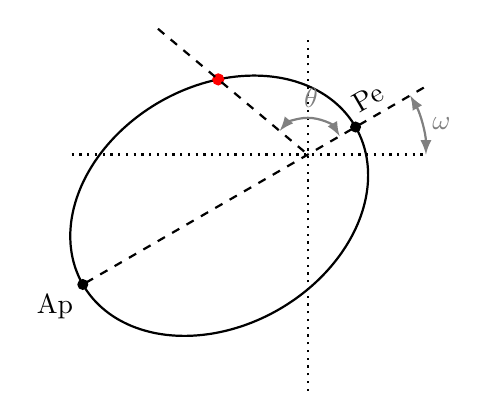
\begin{tikzpicture}[>=latex]
        \def\ecc{0.65}
        \def\SMA{2}
        \def\ap{\fpeval{\SMA*(1+\ecc)}}
        \def\pe{\fpeval{\SMA*(1-\ecc)}}
        \def\omeg{30}
        \def\slr{\fpeval{\SMA*(1-\ecc^2)}}
        \def\arcRad{1.5}
        \def\thta{110}

        \draw[thick, dotted] (-3,0)--(1.5,0);
        \draw[thick, dotted] (0,-3)--(0,1.5);
        \draw[domain=0:2*pi,samples=500, thick] plot ({deg(\x)+\omeg}:{(\slr)/(1+\ecc*cos(\x r))});
        \draw[thick, dashed] (\omeg:\pe+\SMA/2)--(180+\omeg:\ap);
        \draw[thick, <->, gray] (\arcRad,0) arc (0:\omeg:\arcRad) node[midway, right] {$\omega{}$};

        \fill(\omeg: -\ap) circle (2pt) node[below left] {Ap};

        \fill(\omeg: \pe) circle (2pt) node[anchor=center, rotate=\omeg, above right] {Pe};
        \filldraw[red] (\omeg+\thta: \fpeval{\slr/(1+\ecc*cos(deg(\thta)))}) circle (2pt);

        \draw[thick, dashed] (\omeg+\thta:\fpeval{\slr/(1+\ecc*cos(deg(\thta)))}+\SMA/2)--(0,0);
        \draw[thick, <->, gray] (\omeg:2*\pe/3) arc (\omeg:\thta+\omeg:2*\pe/3) node[midway, above] {$\theta$};

    \end{tikzpicture}

    \caption{True Anomaly and Argument of Periapsis}\label{fig:True Anomaly and Arg of Periapsis}
\end{figure}
Above, an orbit is shown with the major axis indicated by a dashed line, and the apoapsis (Ap) and periapsis (Pe) labeled. The origin of this coordinate system is the focus about which the body orbits. The argument of periapsis $\omega$ is the angle between the periapsis of the orbit and the ascending node (the +x axis in this case), and the true anomaly $\theta$ (sometimes designated $\nu$) is the angle between the satellite's current location and its periapsis

\bigskip\bigskip
\subsection{Coordinate Systems}
\begin{figure}[H]
    \centering
    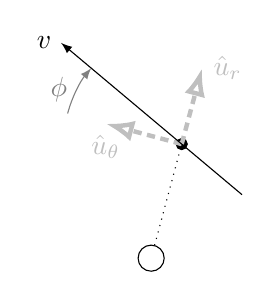
\begin{tikzpicture}[>=latex]
        \def\dist{1.5}
        \def\thta{75}
        \def\unMag{1}
        \def\arcRad{1.5}
        \def\phiAng{25}
        \def\vMag{2}

        \coordinate (rOffs) at (5, 0) {};
        \coordinate (pt) at (\thta:\dist) {};

        \filldraw[] (pt) circle (2pt);

        \draw[dotted] (0,0) -- (pt);
        \draw[densely dashed, -{Latex[open]}, lightgray, ultra thick] (pt) -- +(\thta:\unMag) node[right] {$\hat{u}_r$};
        \draw[densely dashed, -{Latex[open]}, lightgray, ultra thick] (pt) -- +(\thta+90:\unMag) node[below] {$\hat{u}_\theta$};

        \draw[->] (pt) --+(\thta-\phiAng-90:\vMag/2) --+(\thta-\phiAng+90:\vMag)node[left] {$\vv{v}$};

        \draw[->, gray] (pt)+(\thta+90:\arcRad) arc (\thta+90:\thta+90-\phiAng:\arcRad) node[midway, left] {$\phi$};

        \node[circle, fill=white, draw=black] at (0,0) {};
    \end{tikzpicture}
    \qquad
    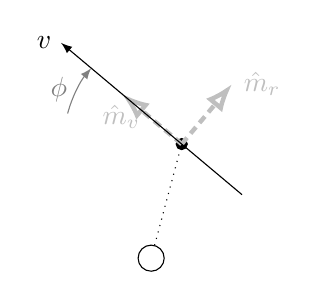
\begin{tikzpicture}[>=latex]
        \def\dist{1.5}
        \def\thta{75}
        \def\unMag{1}
        \def\arcRad{1.5}
        \def\phiAng{25}
        \def\vMag{2}

        \coordinate (rOffs) at (5, 0) {};
        \coordinate (pt) at (\thta:\dist) {};

        \filldraw[] (pt) circle (2pt);

        \draw[dotted] (0,0) -- (pt);
        \draw[densely dashed, -{Latex[open]}, lightgray, ultra thick] (pt) -- +(\thta-\phiAng:\unMag) node[right] {$\hat{m}_r$};
        \draw[densely dashed, -{Latex[open]}, lightgray, ultra thick] (pt) -- +(\thta-\phiAng+90:\unMag) node[below] {$\hat{m}_v$};

        \draw[->] (pt) --+(\thta-\phiAng-90:\vMag/2) --+(\thta-\phiAng+90:\vMag)node[left] {$\vv{v}$};

        \draw[->, gray] (pt)+(\thta+90:\arcRad) arc (\thta+90:\thta+90-\phiAng:\arcRad) node[midway, left] {$\phi$};

        \node[circle, fill=white, draw=black] at (0,0) {};
    \end{tikzpicture}

    \caption{Polar and maneuvering vector frames}\label{fig:Coordinate System}
\end{figure}

A satellite (black dot) is shown orbiting a source (hollow circle) with the flight path angle $\phi$ and velocity vector $\vec{v}$ indicated. On the left image, the polar basis vectors $u$ are shown. On the right, the manuevering vectors $m$ are shown.

The polar basis vectors are defined such that $\hat{u}_r$ points radially outward from the planet, with $\hat{u}_\theta$ being perpendicular to it and generally in the direction of the velocity vector (and in plane with both $\vec{v}$ and $\hat{u}_r$). $\hat{u}_n$ is defined $\hat{u}_n=\hat{u}_r\times\hat{u}_\theta$. In this figure, $\hat{u}_n$ points out-of-page.

The manuevering basis vectors $m$ are defined such that $\hat{m}_v$ points in the direction of the velocity, with $\hat{m}_r$ being normal to it and generally facing away from the planet (and in the plane defined by the velocity vector and the planet). $\hat{m}_n$ will always be equal to $\hat{u}_n$, and is defined as $\hat{m}_n=\hat{m}_r\times\hat{m}_v$.

The flight path angle is the angle between the two basis vectors

\bigskip\bigskip
\subsection{Coordinate System 3D}
\begin{figure}[H]
    \centering
    \def\ecc{0.65}
    \def\SMA{3}
    \def\slr{\fpeval{\SMA*(1-\ecc^2)}}
    \def\ap{\fpeval{\SMA*(1+\ecc)}}
    \def\pe{\fpeval{\SMA*(1-\ecc)}}
    \def\dst{\ap}
    \def\SmA{\fpeval{\SMA*sqrt(1-\ecc^2)}}
    \def\inc{20}

    \tdplotsetmaincoords{70}{30}
    \begin{tikzpicture}[tdplot_main_coords, >=latex]
        \draw[->, green, ultra thick] (0,0,0) -- (2,0,0);
        %\draw[->, red] (0,0,0) -- (0,1,0) node[above]{$y$};
        %\draw[->, red] (0,0,0) -- (0,0,1) node[above]{$z$};
        \draw[densely dashed, gray] (0,0,0) -- (\fpeval{\dst*cos(deg(\inc))},0,0)--+(0,0,\fpeval{\dst*sin(deg(\inc))});

        \tdplotsetrotatedcoords{0}{-\inc}{0}
        \coordinate[tdplot_rotated_coords] (pt) at (3,0,0);

        % orbit
        \draw[tdplot_rotated_coords,samples=500, lightgray] plot ({deg(\x)}:{(\slr)/(1-\ecc*cos(\x r))});
        \draw[tdplot_rotated_coords, gray] (-\pe,0,0) -- (\ap,0,0);
        \draw[tdplot_rotated_coords, gray] (\ecc*\SMA,-\SmA,0) -- (\ecc*\SMA,\SmA,0);

        % Ascending an Descending Nodes
        \filldraw[red] (0,\slr,0) circle (1pt) node[right, black] {\small DN};
        \filldraw[red] (0,-\slr,0) circle (1pt) node[left, black] {\small AN};
        \draw[dotted, red] (0,\slr,0)--(0,-\slr,0);


        % new coord system
        \draw[tdplot_rotated_coords,blue, ->] (\dst,0,0) -- +(1,0,0) node[right]{$\hat{u}_r$};
        \draw[tdplot_rotated_coords,blue, ->] (\dst,0,0) -- +(0,1,0) node[above right]{$\hat{u}_\theta$};
        \draw[tdplot_rotated_coords,blue, ->] (\dst,0,0) -- +(0,0,1) node[above]{$\hat{u}_n$};
        \filldraw[tdplot_rotated_coords] (\dst,0,0) circle (2pt);

        % Inclination Label
        \draw[tdplot_rotated_coords,blue, ->] (0,0,0) -- +(0,0,1) node[left]{$\hat{u}_n$};
        \draw[tdplot_rotated_coords,gray, densely dashed] (0,0,0) -- +(0,0,2);
        \draw[densely dashed, gray] (0,0,0) -- (0,0,2);
        \tdplotsetrotatedcoords{-90}{90}{90}
        \draw[tdplot_rotated_coords, densely dashed, thick] (0,2,0) arc (90:90+\inc:2) node[midway, above] {$i$};
    \end{tikzpicture}

    \caption{Inclined orbit showing the polar basis vectors}\label{fig:Coordinate System 3D}
\end{figure}
A satellite (black dot) is shown above orbiting a body with the polar coordinate system shown. The semi-major and semi-minor axes are shown with a thin line. Note that in this position (at the apoapsis in this case, however this also holds true at periapsis), the polar $u$ and maneuvering $m$ basis vectors are equal.

Note that the inclination $i$ of the orbit is also shown. In this figure the satellite is shown with $\theta=\pi$ and $\omega=\frac{3}{2}\pi$ (the satellite is 180 degrees offset from its periapsis, and the periapsis is 270 degrees offset from the ascending node). The red dots are the ascending and descending nodes. These are the points at which the orbit intersects the horizon. The ascending node (AN) is the one at which the latitude changes from negative to positive, and the desending node (DN) is the point at which latitude goes from positive to negative. In this figure, $\Omega=\frac{3}{2}\pi$ (with the reference direction being the green arrow). Note that $\Omega$ does not always equal $\omega$; $\Omega$ positions the ascending node relative to a reference direction, while $\omega$ positions the periapsis relative to the ascending node.


\end{document}